% The master copy of this demo dissertation is held on my filespace
% on the cl file serve (/homes/mr/teaching/demodissert/)

% Last updated by PMY on 3 March 2012

\documentclass[12pt,twoside,notitlepage,xetex]{report}

\usepackage{a4}
\usepackage{verbatim}
\usepackage{epsf}
\usepackage{sectsty}

\usepackage{url}
\usepackage{parskip}
\usepackage{pdfpages}
% \usepackage{wrapfig}
\usepackage{subfig}
\usepackage[normalem]{ulem}
\usepackage{caption}
\usepackage{color}
\usepackage{float}
% \usepackage{lettrine} % dropped capitals at start of chapter
\usepackage{fancyvrb}
% \usepackage{cprotect}
\usepackage{lscape}
\usepackage{multirow}

\usepackage{graphicx}
\usepackage{fontspec,xunicode}
\defaultfontfeatures{Mapping=tex-text, Numbers=Monospaced}% ,Scale=MatchLowercase% , Numbers=OldStyle
\setmainfont[Scale=1]{Linux Libertine O}% {Sabon MT Std}
\setsansfont{Roboto Bold}% {Myriad Pro Light}
\setmonofont[Scale=0.82]{Monaco}% {Droid Sans Mono}
\allsectionsfont{\sffamily}

\newfontinstance\bigsf[Color=000000,Scale=1.25]{Roboto Bold}% {Myriad Pro Light}
\newfontinstance\sfapp[Color=000000,Scale=0.82]{Roboto Regular}% {Myriad Pro Light}

\definecolor{red}{rgb}{0.80,0.00,0.00}
\definecolor{green}{rgb}{0.00,0.80,0.00}
\definecolor{blue}{rgb}{0.00,0.00,0.80}

%%% ====================================================================
%%%   This file is freely redistributable and placed into the
%%%   public domain by Tomas Rokicki.
%%%  @TeX-file{
%%%     author          = "Tom Rokicki",
%%%     version         = "2.7k",
%%%     date            = "19 July 1997",
%%%     time            = "10:00:05 MDT",
%%%     filename        = "epsf.tex",
%%%     address         = "Tom Rokicki
%%%                        Box 2081
%%%                        Stanford, CA 94309
%%%                        USA",
%%%     telephone       = "+1 415 855 9989",
%%%     email           = "rokicki@cs.stanford.edu (Internet)",
%%%     codetable       = "ISO/ASCII",
%%%     keywords        = "PostScript, TeX",
%%%     supported       = "yes",
%%%     abstract        = "This file contains macros to support the inclusion
%%%                        of Encapsulated PostScript files in TeX documents.",
%%%     docstring       = "This file contains TeX macros to include an
%%%                        Encapsulated PostScript graphic.  It works
%%%                        by finding the bounding box comment,
%%%                        calculating the correct scale values, and
%%%                        inserting a vbox of the appropriate size at
%%%                        the current position in the TeX document.
%%%
%%%                        To use, simply say
%%%
%%%                        \input epsf % somewhere early on in your TeX file
%%%
%%%                        % then where you want to insert a vbox for a figure:
%%%                        \epsfbox{filename.ps}
%%%
%%%                        Alternatively, you can supply your own
%%%                        bounding box by
%%%
%%%                        \epsfbox[0 0 30 50]{filename.ps}
%%%
%%%                        This will not read in the file, and will
%%%                        instead use the bounding box you specify.
%%%
%%%                        The effect will be to typeset the figure as
%%%                        a TeX box, at the point of your \epsfbox
%%%                        command. By default, the graphic will have
%%%                        its `natural' width (namely the width of
%%%                        its bounding box, as described in
%%%                        filename.ps). The TeX box will have depth
%%%                        zero.
%%%
%%%                        You can enlarge or reduce the figure by
%%%                        saying
%%%
%%%                          \epsfxsize=<dimen> \epsfbox{filename.ps}
%%%                        or
%%%                          \epsfysize=<dimen> \epsfbox{filename.ps}
%%%
%%%                        instead. Then the width of the TeX box will
%%%                        be \epsfxsize and its height will be scaled
%%%                        proportionately (or the height will be
%%%                        \epsfysize and its width will be scaled
%%%                        proportionately).
%%%
%%%                        The width (and height) is restored to zero
%%%                        after each use, so \epsfxsize or \epsfysize
%%%                        must be specified before EACH use of
%%%                        \epsfbox.
%%%
%%%                        A more general facility for sizing is
%%%                        available by defining the \epsfsize macro.
%%%                        Normally you can redefine this macro to do
%%%                        almost anything.  The first parameter is
%%%                        the natural x size of the PostScript
%%%                        graphic, the second parameter is the
%%%                        natural y size of the PostScript graphic.
%%%                        It must return the xsize to use, or 0 if
%%%                        natural scaling is to be used.  Common uses
%%%                        include:
%%%
%%%                           \epsfxsize  % just leave the old value alone
%%%                           0pt         % use the natural sizes
%%%                           #1          % use the natural sizes
%%%                           \hsize      % scale to full width
%%%                           0.5#1       % scale to 50% of natural size
%%%                           \ifnum #1>\hsize\hsize\else#1\fi
%%%                                       % smaller of natural, hsize
%%%
%%%                        If you want TeX to report the size of the
%%%                        figure (as a message on your terminal when
%%%                        it processes each figure), say
%%%                        `\epsfverbosetrue'.
%%%
%%%                        If you only want to get the bounding box
%%%                        extents, without producing any output boxes
%%%                        or \special{}, then say
%%%                        \epsfgetbb{filename}.  The extents will be
%%%                        saved in the macros \epsfllx \epsflly
%%%                        \epsfurx \epsfury in PostScript units of
%%%                        big points.
%%%
%%%                        Revision history:
%%%
%%%                        ---------------------------------------------
%%%                        epsf.tex macro file:
%%%                        Originally written by Tomas Rokicki of
%%%                        Radical Eye Software, 29 Mar 1989.
%%%
%%%                        ---------------------------------------------
%%%                        Revised by Don Knuth, 3 Jan 1990.
%%%
%%%                        ---------------------------------------------
%%%                        Revised by Tomas Rokicki, 18 Jul 1990.
%%%                        Accept bounding boxes with no space after
%%%                        the colon.
%%%
%%%                        ---------------------------------------------
%%%                        Revised by Nelson H. F. Beebe
%%%                        <beebe@math.utah.edu>, 03 Dec 1991 [2.0].
%%%                        Add version number and date typeout.
%%%
%%%                        Use \immediate\write16 instead of \message
%%%                        to ensure output on new line.
%%%
%%%                        Handle nested EPS files.
%%%
%%%                        Handle %%BoundingBox: (atend) lines.
%%%
%%%                        Do not quit when blank lines are found.
%%%
%%%                        Add a few percents to remove generation of
%%%                        spurious blank space.
%%%
%%%                        Move \special output to
%%%                        \epsfspecial{filename} so that other macro
%%%                        packages can input this one, then change
%%%                        the definition of \epsfspecial to match
%%%                        another DVI driver.
%%%
%%%                        Move size computation to \epsfsetsize which
%%%                        can be called by the user; the verbose
%%%                        output of the bounding box and scaled width
%%%                        and height happens here.
%%%
%%%                        ---------------------------------------------
%%%                        Revised by Nelson H. F. Beebe
%%%                        <beebe@math.utah.edu>, 05 May 1992 [2.1].
%%%                        Wrap \leavevmode\hbox{} around \vbox{} with
%%%                        the \special so that \epsffile{} can be
%%%                        used inside \begin{center}...\end{center}
%%%
%%%                        ---------------------------------------------
%%%                        Revised by Nelson H. F. Beebe
%%%                        <beebe@math.utah.edu>, 09 Dec 1992 [2.2].
%%%                        Introduce \epsfshow{true,false} and
%%%                        \epsfframe{true,false} macros; the latter
%%%                        suppresses the insertion of the PostScript,
%%%                        and instead just creates an empty box,
%%%                        which may be handy for rapid prototyping.
%%%
%%%                        ---------------------------------------------
%%%                        Revised by Nelson H. F. Beebe
%%%                        <beebe@math.utah.edu>, 14 Dec 1992 [2.3].
%%%                        Add \epsfshowfilename{true,false}.  When
%%%                        true, and \epsfshowfalse is specified, the
%%%                        PostScript file name will be displayed
%%%                        centered in the figure box.
%%%
%%%                        ---------------------------------------------
%%%                        Revised by Nelson H. F. Beebe
%%%                        <beebe@math.utah.edu>, 20 June 1993 [2.4].
%%%                        Remove non-zero debug setting of \epsfframemargin,
%%%                        and change margin handling to preserve EPS image
%%%                        size and aspect ratio, so that the actual
%%%                        box is \epsfxsize+\epsfframemargin wide by
%%%                        \epsfysize+\epsfframemargin high.
%%%                        Reduce output of \epsfshowfilenametrue to
%%%                        just the bare file name.
%%%
%%%                        ---------------------------------------------
%%%                        Revised by Nelson H. F. Beebe
%%%                        <beebe@math.utah.edu>, 13 July 1993 [2.5].
%%%                        Add \epsfframethickness for control of
%%%                        \epsfframe frame lines.
%%%
%%%                        ---------------------------------------------
%%%                        Revised by Nelson H. F. Beebe
%%%                        <beebe@math.utah.edu>, 02 July 1996 [2.6]
%%%                        Add missing initialization \epsfatendfalse;
%%%                        the lack of this resulted in the wrong
%%%                        BoundingBox being picked up, mea culpa, sigh...
%%%                        ---------------------------------------------
%%%
%%%                        ---------------------------------------------
%%%                        Revised by Nelson H. F. Beebe
%%%                        <beebe@math.utah.edu>, 25 October 1996 [2.7]
%%%                        Update to match changes in from dvips 5-600
%%%                        distribution: new user-accessible macros:
%%%                        \epsfclipon, \epsfclipoff, \epsfdrafton,
%%%                        \epsfdraftoff, change \empty to \epsfempty.
%%%                        ---------------------------------------------
%%%                        
%%%                        Modified to avoid verbosity, give help.
%%%                        --kb@cs.umb.edu, for Texinfo.
%%%  }
%%% ====================================================================
%
\ifx\epsfannounce\undefined \def\epsfannounce{\immediate\write16}\fi
 \epsfannounce{This is `epsf.tex' v2.7k <10 July 1997>}%
%
\newread\epsffilein    % file to \read
\newif\ifepsfatend     % need to scan to LAST %%BoundingBox comment?
\newif\ifepsfbbfound   % success?
\newif\ifepsfdraft     % use draft mode?
\newif\ifepsffileok    % continue looking for the bounding box?
\newif\ifepsfframe     % frame the bounding box?
\newif\ifepsfshow      % show PostScript file, or just bounding box?
\epsfshowtrue          % default is to display PostScript file
\newif\ifepsfshowfilename % show the file name if \epsfshowfalse specified?
\newif\ifepsfverbose   % report what you're making?
\newdimen\epsfframemargin % margin between box and frame
\newdimen\epsfframethickness % thickness of frame rules
\newdimen\epsfrsize    % vertical size before scaling
\newdimen\epsftmp      % register for arithmetic manipulation
\newdimen\epsftsize    % horizontal size before scaling
\newdimen\epsfxsize    % horizontal size after scaling
\newdimen\epsfysize    % vertical size after scaling
\newdimen\pspoints     % conversion factor
%
\pspoints = 1bp        % Adobe points are `big'
\epsfxsize = 0pt       % default value, means `use natural size'
\epsfysize = 0pt       % ditto
\epsfframemargin = 0pt % default value: frame box flush around picture
\epsfframethickness = 0.4pt % TeX's default rule thickness
%
\def\epsfbox#1{\global\def\epsfllx{72}\global\def\epsflly{72}%
   \global\def\epsfurx{540}\global\def\epsfury{720}%
   \def\lbracket{[}\def\testit{#1}\ifx\testit\lbracket
   \let\next=\epsfgetlitbb\else\let\next=\epsfnormal\fi\next{#1}}%
%
% We use \epsfgetlitbb if the user specified an explicit bounding box,
% and \epsfnormal otherwise.  Because \epsfgetbb can be called
% separately to retrieve the bounding box, we move the verbose
% printing the bounding box extents and size on the terminal to
% \epsfstatus.  Therefore, when the user provided the bounding box,
% \epsfgetbb will not be called, so we must call \epsfsetsize and
% \epsfstatus ourselves.
%
\def\epsfgetlitbb#1#2 #3 #4 #5]#6{%
   \epsfgrab #2 #3 #4 #5 .\\%
   \epsfsetsize
   \epsfstatus{#6}%
   \epsfsetgraph{#6}%
}%
%
\def\epsfnormal#1{%
    \epsfgetbb{#1}%
    \epsfsetgraph{#1}%
}%
%
\newhelp\epsfnoopenhelp{The PostScript image file must be findable by
TeX, i.e., somewhere in the TEXINPUTS (or equivalent) path.}%
%
\def\epsfgetbb#1{%
%
%   The first thing we need to do is to open the
%   PostScript file, if possible.
%
    \openin\epsffilein=#1
    \ifeof\epsffilein
        \errhelp = \epsfnoopenhelp
        \errmessage{Could not open file #1, ignoring it}%
    \else                       %process the file
        {%                      %start a group to contain catcode changes
            % Make all special characters, except space, to be of type
            % `other' so we process the file in almost verbatim mode
            % (TeXbook, p. 344).
            \chardef\other=12
            \def\do##1{\catcode`##1=\other}%
            \dospecials
            \catcode`\ =10
            \epsffileoktrue         %true while we are looping
            \epsfatendfalse     %[02-Jul-1996]: add forgotten initialization
            \loop               %reading lines from the EPS file
                \read\epsffilein to \epsffileline
                \ifeof\epsffilein %then no more input
                \epsffileokfalse %so set completion flag
            \else                %otherwise process one line
                \expandafter\epsfaux\epsffileline:. \\%
            \fi
            \ifepsffileok
            \repeat
            \ifepsfbbfound
            \else
                \ifepsfverbose
                    \immediate\write16{No BoundingBox comment found in %
                                    file #1; using defaults}%
                \fi
            \fi
        }%                      %end catcode changes
        \closein\epsffilein
    \fi                         %end of file processing
    \epsfsetsize                %compute size parameters
    \epsfstatus{#1}%
}%
%
% Clipping control:
\def\epsfclipon{\def\epsfclipstring{ clip}}%
\def\epsfclipoff{\def\epsfclipstring{\ifepsfdraft\space clip\fi}}%
\epsfclipoff % default for dvips is OFF
%
% The special that is emitted by \epsfsetgraph comes from this macro.
% It is defined separately to allow easy customization by other
% packages that first \input epsf.tex, then redefine \epsfspecial.
% This macro is invoked in the lower-left corner of a box of the
% width and height determined from the arguments to \epsffile, or
% from the %%BoundingBox in the EPS file itself.
%
% This version is for dvips:
\def\epsfspecial#1{%
     \epsftmp=10\epsfxsize
     \divide\epsftmp\pspoints
     \ifnum\epsfrsize=0\relax
       \special{PSfile=\ifepsfdraft psdraft.ps\else#1\fi\space
                llx=\epsfllx\space
                lly=\epsflly\space
                urx=\epsfurx\space
                ury=\epsfury\space
                rwi=\number\epsftmp
                \epsfclipstring
               }%
     \else
       \epsfrsize=10\epsfysize
       \divide\epsfrsize\pspoints
       \special{PSfile=\ifepsfdraft psdraft.ps\else#1\fi\space
                llx=\epsfllx\space
                lly=\epsflly\space
                urx=\epsfurx\space
                ury=\epsfury\space
                rwi=\number\epsftmp\space
                rhi=\number\epsfrsize
                \epsfclipstring
               }%
     \fi
}%
%
% \epsfframe macro adapted from the TeXbook, exercise 21.3, p. 223, 331.
% but modified to set the box width to the natural width, rather
% than the line width, and to include space for margins and rules
\def\epsfframe#1%
{%
  \leavevmode                   % so we can put this inside
                                % a centered environment
  \setbox0 = \hbox{#1}%
  \dimen0 = \wd0                                % natural width of argument
  \advance \dimen0 by 2\epsfframemargin         % plus width of 2 margins
  \advance \dimen0 by 2\epsfframethickness      % plus width of 2 rule lines
  \vbox
  {%
    \hrule height \epsfframethickness depth 0pt
    \hbox to \dimen0
    {%
      \hss
      \vrule width \epsfframethickness
      \kern \epsfframemargin
      \vbox {\kern \epsfframemargin \box0 \kern \epsfframemargin }%
      \kern \epsfframemargin
      \vrule width \epsfframethickness
      \hss
    }% end hbox
    \hrule height 0pt depth \epsfframethickness
  }% end vbox
}%
%
\def\epsfsetgraph#1%
{%
   %
   % Make the vbox and stick in a \special that the DVI driver can
   % parse.  \vfil and \hfil are used to place the \special origin at
   % the lower-left corner of the vbox.  \epsfspecial can be redefined
   % to produce alternate \special syntaxes.
   %
   \leavevmode
   \hbox{% so we can put this in \begin{center}...\end{center}
     \ifepsfframe\expandafter\epsfframe\fi
     {\vbox to\epsfysize
     {%
        \ifepsfshow
            % output \special{} at lower-left corner of figure box
            \vfil
            \hbox to \epsfxsize{\epsfspecial{#1}\hfil}%
        \else
            \vfil
            \hbox to\epsfxsize{%
               \hss
               \ifepsfshowfilename
               {%
                  \epsfframemargin=3pt % local change of margin
                  \epsfframe{{\tt #1}}%
               }%
               \fi
               \hss
            }%
            \vfil
        \fi
     }%
   }}%
   %
   % Reset \epsfxsize and \epsfysize, as documented above.
   %
   \global\epsfxsize=0pt
   \global\epsfysize=0pt
}%
%
%   Now we have to calculate the scale and offset values to use.
%   First we compute the natural sizes.
%
\def\epsfsetsize
{%
   \epsfrsize=\epsfury\pspoints
   \advance\epsfrsize by-\epsflly\pspoints
   \epsftsize=\epsfurx\pspoints
   \advance\epsftsize by-\epsfllx\pspoints
%
%   If `epsfxsize' is 0, we default to the natural size of the picture.
%   Otherwise we scale the graph to be \epsfxsize wide.
%
   \epsfxsize=\epsfsize{\epsftsize}{\epsfrsize}%
   \ifnum \epsfxsize=0
      \ifnum \epsfysize=0
        \epsfxsize=\epsftsize
        \epsfysize=\epsfrsize
        \epsfrsize=0pt
%
%   We have a sticky problem here:  TeX doesn't do floating point arithmetic!
%   Our goal is to compute y = rx/t. The following loop does this reasonably
%   fast, with an error of at most about 16 sp (about 1/4000 pt).
%
      \else
        \epsftmp=\epsftsize \divide\epsftmp\epsfrsize
        \epsfxsize=\epsfysize \multiply\epsfxsize\epsftmp
        \multiply\epsftmp\epsfrsize \advance\epsftsize-\epsftmp
        \epsftmp=\epsfysize
        \loop \advance\epsftsize\epsftsize \divide\epsftmp 2
        \ifnum \epsftmp>0
           \ifnum \epsftsize<\epsfrsize
           \else
              \advance\epsftsize-\epsfrsize \advance\epsfxsize\epsftmp
           \fi
        \repeat
        \epsfrsize=0pt
      \fi
   \else
     \ifnum \epsfysize=0
       \epsftmp=\epsfrsize \divide\epsftmp\epsftsize
       \epsfysize=\epsfxsize \multiply\epsfysize\epsftmp
       \multiply\epsftmp\epsftsize \advance\epsfrsize-\epsftmp
       \epsftmp=\epsfxsize
       \loop \advance\epsfrsize\epsfrsize \divide\epsftmp 2
       \ifnum \epsftmp>0
          \ifnum \epsfrsize<\epsftsize
          \else
             \advance\epsfrsize-\epsftsize \advance\epsfysize\epsftmp
          \fi
       \repeat
       \epsfrsize=0pt
     \else
       \epsfrsize=\epsfysize
     \fi
   \fi
}%
%
% Issue some status messages if the user requested them
%
\def\epsfstatus#1{% arg = filename
   \ifepsfverbose
     \immediate\write16{#1: BoundingBox:
                  llx = \epsfllx\space lly = \epsflly\space
                  urx = \epsfurx\space ury = \epsfury\space}%
     \immediate\write16{#1: scaled width = \the\epsfxsize\space
                  scaled height = \the\epsfysize}%
   \fi
}%
%
%   We still need to define the tricky \epsfaux macro. This requires
%   a couple of magic constants for comparison purposes.
%
{\catcode`\%=12 \global\let\epsfpercent=%\global\def\epsfbblit{%BoundingBox}}%
\global\def\epsfatend{(atend)}%
%
%   So we're ready to check for `%BoundingBox:' and to grab the
%   values if they are found.
%
%   If we find a line
%
%   %%BoundingBox: (atend)
%
%   then we ignore it, but set a flag to force parsing all of the
%   file, so the last %%BoundingBox parsed will be the one used.  This
%   is necessary, because EPS files can themselves contain other EPS
%   files with their own %%BoundingBox comments.
%
%   If we find a line
%
%   %%BoundingBox: llx lly urx ury
%
%   then we save the 4 values in \epsfllx, \epsflly, \epsfurx, \epsfury.
%   Then, if we have not previously parsed an (atend), we flag completion
%   and can stop reading the file.  Otherwise, we must keep on reading
%   to end of file so that we find the values on the LAST %%BoundingBox.
\long\def\epsfaux#1#2:#3\\%
{%
   \def\testit{#2}%             % save second character up to just before colon
   \ifx#1\epsfpercent           % then first char is percent (quick test)
       \ifx\testit\epsfbblit    % then (slow test) we have %%BoundingBox
            \epsfgrab #3 . . . \\%
            \ifx\epsfllx\epsfatend % then ignore %%BoundingBox: (atend)
                \global\epsfatendtrue
            \else               % else found %%BoundingBox: llx lly urx ury
                \ifepsfatend    % then keep parsing ALL %%BoundingBox lines
                \else           % else stop after first one parsed
                    \epsffileokfalse
                \fi
                \global\epsfbbfoundtrue
            \fi
       \fi
   \fi
}%
%
%   Here we grab the values and stuff them in the appropriate definitions.
%
\def\epsfempty{}%
\def\epsfgrab #1 #2 #3 #4 #5\\{%
   \global\def\epsfllx{#1}\ifx\epsfllx\epsfempty
      \epsfgrab #2 #3 #4 #5 .\\\else
   \global\def\epsflly{#2}%
   \global\def\epsfurx{#3}\global\def\epsfury{#4}\fi
}%
%
%   We default the epsfsize macro.
%
\def\epsfsize#1#2{\epsfxsize}%
%
%   Finally, another definition for compatibility with older macros.
%
\let\epsffile=\epsfbox
\endinput
                            % to allow postscript inclusions
% On thor and CUS read top of file:
%     /opt/TeX/lib/texmf/tex/dvips/epsf.sty
% On CL machines read:
%     /usr/lib/tex/macros/dvips/epsf.tex

\raggedbottom                           % try to avoid widows and orphans
\raggedright                            % left-aligned, not justified
\sloppy
\clubpenalty1000%
\widowpenalty1000%

\addtolength{\oddsidemargin}{6mm}       % adjust margins
\addtolength{\evensidemargin}{-8mm}

\renewcommand{\baselinestretch}{1.1}    % adjust line spacing to make
                                        % more readable

\renewcommand{\captionfont}{\footnotesize}

\setcounter{secnumdepth}{5}
% \setcounter{tocdepth}{5}

\begin{document}
\nocite{*}
\bibliographystyle{plain}% {unsrt}


%%%%%%%%%%%%%%%%%%%%%%%%%%%%%%%%%%%%%%%%%%%%%%%%%%%%%%%%%%%%%%%%%%%%%%%%
% Title


\pagestyle{empty}

% \hfill{\LARGE \bf \sffamily Philip Yeeles}
\hfill{\Large Philip Yeeles}

\vspace*{60mm}
\begin{center}
\LARGE
{\bf \bigsf Nico: An Environment for Mathematical Expression in Schools}\\
\vspace*{5mm}
% {\sffamily Computer Science Tripos} \\
Computer Science Tripos\\
\vspace*{5mm}
% {\sffamily Selwyn College} \\
Selwyn College\\
\vspace*{5mm}
% {\sffamily \today}  % today's date
\today % today's date
\end{center}

\cleardoublepage

%%%%%%%%%%%%%%%%%%%%%%%%%%%%%%%%%%%%%%%%%%%%%%%%%%%%%%%%%%%%%%%%%%%%%%%%%%%%%%
% Proforma, table of contents and list of figures

\setcounter{page}{1}
\pagenumbering{roman}
\pagestyle{plain}

\chapter*{Proforma}

{\large
\begin{tabular}{ll}
\bf Name:               & Philip Yeeles                                                   \\
\bf College:            & Selwyn College                                                  \\
\bf Project Title:      & Nico: An Environment for Mathematical\\
                        & Expression in Schools \\
\bf Examination:        & Computer Science Tripos, May 2012                               \\
\bf Word Count:         & TBC\footnotemark[1]
(well less than the 12000 limit) \\
\bf Project Originator: & P.~M.~Yeeles (\verb¬pmy22¬)                                    \\
\bf Supervisors:        & Dr S.~J.~Aaron (\verb¬sja55¬), A.~G.~Stead (\verb¬ags46¬)     \\
\end{tabular}
}
\footnotetext[1]{This word count was computed using the web interface to {\ttfamily texcount}, which can be found at \url{http://app.uio.no/ifi/texcount/online.php}.}
\stepcounter{footnote}


\section*{Original Aims of the Project}

The aim of this project was to develop an application to act as an aid in mathematical education for pupils in Year 5.  The software was to provide a new graphical metaphor for calculation with an accompanying working environment, with the intention of eliminating some of the problems that makes handwritten arithmetic unclear in many situations.

%The aim of the project was to develop an application in the Clojure programming
%language which would allow users to express mathematical calculations using a
%graphical notation.  The software was to be able to generate an abstract syntax
%tree from the graphical notation, evaluate it and pass the results back to the
%application in under 300ms.  An extension to the project was to conduct a user
%study to evaluate the utility of the software.

\section*{Work Completed}

I have successfully designed and implemented an application using the Clojure programming language that allows users to express calculations using a graphical notation.  The software is able to generate an abstract syntax tree from the graphical notation, evaluate it and pass the results back to the application in approximately 10ms.  As an extension to the project, a user study was conducted to evaluate the utility of the software.

%I have successfully designed and implemented the application detailed in the
%previous section.  That is, I have developed an application in which it is
%possible to express calculations using a graphical notation, that generates an
%abstract syntax tree from the language and that is able to parse the tree and
%return the results in under 300ms.  I have also conducted a user study to assess
%whether or not the software is actually of use with regard to mathematics
%education.

\section*{Special Difficulties}

\begin{itemize}
\item Learning the Clojure programming language % TODO: expand
\item Learning to choose appropriate mutable data structures of those that Clojure provides
\item Learning to incorporate tests into the development cycle
\end{itemize}

\newpage
\section*{Declaration of Originality}

I, Philip Michael Yeeles of Selwyn College, being a candidate for Part
II of the Computer Science Tripos, hereby declare that this dissertation
and the work described in it are my own work, unaided except as may be
specified below, and that the dissertation does not contain material
that has already been used to any substantial extent for a comparable
purpose.

\bigskip
\leftline{Signed}

\medskip
\leftline{Date \today}

\cleardoublepage

\tableofcontents

\listoffigures

\newpage
\section*{Acknowledgements}
My thanks to Luke Church for his advice regarding user studies, and to Alistair
Stead and Sam Aaron for their encouragement and patience.

%%%%%%%%%%%%%%%%%%%%%%%%%%%%%%%%%%%%%%%%%%%%%%%%%%%%%%%%%%%%%%%%%%%%%%%
% now for the chapters

\cleardoublepage        % just to make sure before the page numbering
                        % is changed

\setcounter{page}{1}
\pagenumbering{arabic}
\pagestyle{headings}

\chapter{Introduction}
% TODO: sort out cogdims: apparently the proper way to do it is to mention cogdims and cite petra & green, then put all the cogdims terms in italics

The aim of this project has been to design and develop a notation and accompanying application to act as a learning aid for pre-algebra arithmetic in schools.  Using Petre and Green's `Cognitive Dimensions' framework as a means of evaluation, the project aims to increase the \emph{visibility} of the notation, to reduce the number of \emph{hidden dependencies} between units of notation, to reduce the \emph{viscosity} of the notation, and to make the flow of data obvious to the user \cite{Green1996}.  I have successfully developed such a system, intended initially for pupils in Year 5 (though extensible, through the creation of alternative question sets, to other age groups), and, as an extension, conducted a user study to assess its utility.

In this chapter, I will discuss my motivations for choosing this project, the pros and cons of the handwritten system it is attempting to augment, the technical challenges involved in developing such a system and related work that has previously been conducted with similar goals.

\section{Motivations}
% evaluation of problems with writing it down on paper
% cogdims of handwritten method(s)
% system requirements (cogdims)

My motivations behind this project lay in the limitations of the handwritten approach to solving mathematical problems that I have observed both in my own learning and in my own teaching experience.  What follows is an assessment of the technical challenges involved in this project, followed by a discussion of the ideal properties of a useful alternative notation.

\pagebreak

% \subsection{Evaluation of the Handwritten Approach}
% % moved to chapter 2 requirements analysis

% \subsection{Requirements of a Replacement System}
% % moved to chapter 2 requirements analysis

\section{Technical Challenges}
% need first-class functions
% need to be able to pass expressions around to evaluate at will: hence functional, hence lisp - homoiconicity
% also need good gui libraries for app - familiar with java/swing so that works (esp. with seesaw), also the option of jfx2 and swt/guiftw
% difficulty of learning clojure over summer in preparation

Developing such an application comprises three main challenges.  Firstly, developing an infrastructure that is capable of creating, storing, editing, deleting, evaluating and nesting calculations.  Secondly, developing an interaction-handler layer that is able to interpret user input and events occurring in the user interface.  Finally, implementing a graphical user interface that is able to render calculations into the devised notation, and allow the user to perform operations upon the notation that affect the underlying calculation.  Such an interface should also be able to display and update the results of a calculation with low latency (a limit of 300ms is set and discussed in footnote 1, \emph{Sec. 2.1.2})).

The application described above must be portable, to account for the diversity of computing environments available to the target audience.  It must also provide a standardised user experience across the platforms on which it is deployed.  A Java-based application satisfies both of these requirements, as any platform on which the Java Virtual Machine (JVM) can be installed is able to run it.  Java also makes GUI libraries available, such as JavaFX and Swing, that are explicitly designed to provide similar GUI functionality on many platforms.

The application would also benefit from functional programming paradigms such as immutability, which results in functions that behave predictably and are easy to test; and homoiconicity, in which data structures can be evaluated as code and code as data structures, allowing mathematical method to be represented in a form that can be interpreted and manipulated by the application.

The Clojure language meets both of the above requirements, being a dialect of LISP that compiles to JVM bytecode.  This gives the developer access to the Java standard library and offers the portability afforded by Java, whilst also providing the benefits of a homoiconic, functional language as described above.  It also has the added benefit of being efficient, as it compiles directly to JVM bytecode.

\section{Previous Work}
% scrubbing calculator http://worrydream.com/ScrubbingCalculator/
% soulver http://www.acqualia.com/soulver/
% neither really targeted at education
% cool stuff at http://worrydream.com/KillMath/ though
% maybe refer to this? http://betterexplained.com/articles/rethinking-arithmetic-a-visual-guide/
% also, this: http://www.ralph-abraham.org/articles/Blurbs/blurb126.shtml
% also, check out espresso and education city stuff, log in to fronter via st. mary's site, uname jyeele1.314, pword b3ach7
% plenty of work been done in making computer maths like paper maths, but not so much the reverse, case in point: http://www.macresearch.org/showcase-review-pi-cubed-iphone-ipod-touch
% also a lot of crap maths games that are essentially a series of qs in disguise, see http://www.time4learning.com/curriculum/try_demos.html
% nico is unabashedly *not* a game, rather a tool, much like a pen or calculator
% problem with calculators?

There already exists a wide variety of educational software for mathematics, which often present mathematical problems in the context of a computer game.  Although such games have repeatedly been shown to be of benefit to the learner, a barrier to their widespread use in education can be the users' preconceptions about the educational value of computer games \cite{Swan2009} \cite{Delacruz2010}.  Indeed, Bragg notes that
\begin{center}
\parbox[c]{\textwidth-2cm}{
\small
``One barrier [...] may be possible negative attitudes held by students towards the likelihood of the games' effectiveness in assisting mathematical learning.'' \cite{Bragg2006}
}
\end{center}
This is reinforced in a later paper by the same author, where Bragg concludes that
\begin{center}
\parbox[c]{\textwidth-2cm}{
\small
``It appeared that game-playing negatively affected attitudes'' \cite{Bragg2007}
}
\end{center}
Although it was also concluded that such problems could be addressed by dedicating lesson time to explaining the educational benefits of game-playing, an alternative approach is to introduce software into the classroom as a {\bf tool}, rather than `just a game'.  In the same way that calculators are used in mathematics lessons, it is the intention of this project to introduce a new tool to complement learning.

There also exist a few applications intended to represent calculations on a computer in novel ways.  A relatively common approach to this has been to try to make on-screen calculations more like on-paper calculations.  One such example is \emph{Pi Cubed}, which tries to make complex calculations appear as they would be written in an exam or exercise book \cite{PiCubed}.  \emph{Soulver}, conversely, tries to achieve this by simulating `back-of-the-envelope' calculations, whereby notes in English augment the calculation \cite{Soulver}.

% TODO: image?  but copyright issues...
Another approach is that of the \emph{Scrubbing Calculator}, which extends the \emph{Soulver}-style environment by helping the user to solve equations by dragging values to edit them, showing how changing a value affects the overall result \cite{ScrubCalc}.  Values can be linked by dragging a line between them, which means that they are two instances of the same value: dragging one changes the value at every location in which it appears.  This is a neat means of visualising equations, but it, too, is not intended for use in education, and still requires the user to be able to formulate an equation.  The \emph{Scrubbing Calculator} is more a tool for facilitating algebraic, rather than arithmetic, understanding; indeed, it is inherently a {\bf calculator}, and so does not encourage thinking about a method of manual calculation.

\section{Summary}
% need a system that incorporates these features: foo, bar, baz, quux

Existing educational games for mathematics, although valid as a pedagogical tool, face obstacles from teachers' and pupils' attitudes toward them, as a result of their status as `just games'.  There exists software to aid in calculation and arithmetic by representing it clearly, but it is not intended for classroom use, and often its purpose is to make on-screen calculations simulate handwritten ones.  An application is proposed to complement teaching, as one would use a calculator in the classroom.  There is a niche for a tool for use in education that represents calculations in a visual manner, with a particular focus on making mathematical {\bf method} clear.  The application is to provide such an environment, in which the user can explore the many ways in which a problem can be solved using a novel graphical notation.% TODO: emphasise? wtf

\cleardoublepage



\chapter{Preparation}

% In this chapter I will discuss the work that was done prior to beginning the
% project proper.  This includes learning the Clojure programming language and
% researching and auditioning graphical metaphors for calculation.  This chapter
% comprises a requirements analysis, followed by an overview of the system
% architecture and a discussion of the additional tools used in the development of
% the project.
This chapter concerns the work that was completed prior to development.  It comprises a requirements analysis, followed by a discussion of the prototyping of the graphical notation that was to be implemented in the final application.

\section{Requirements Analysis}
% http://www.cs.fsu.edu/~lacher/courses/COP3331/rad.html
% http://www.nd.gov/itd/files/services/pm/requirements-analysis-guidebook.pdf
% TODO: write about the requirements analysis and why we're doing one

\subsection{Current System}
% move evaluation of handwritten arithmetic from chapter 1 here?

\begin{figure}
% \begin{wrapfigure}{r}{0.5\textwidth}
\begin{center}
\subfloat[]{
\parbox{2cm}{
\begin{center}
{\small
24+35=59\\
12+48=60\\
59+72=131\\
1+60=61\\
131+61=192}
\end{center}}}
\subfloat[]{
\parbox{2cm}{
\begin{center}
{\small
24+35={\color{green}59}\\
12+48={\color{blue}60}\\
{\color{green}59}+72={\color{green}131}\\
1+{\color{blue}60}={\color{blue}61}\\
{\color{green}131}+{\color{blue}61}=192}
\end{center}}}
\subfloat[]{
\parbox{4cm}{
\begin{center}
{\small
24+35= {\color{red}\sout{59}} {\color{green}49}\\
12+48={\color{blue}60}\\
{\color{red}\sout{59}} {\color{green}49}+72= {\color{red}\sout{131}} {\color{green}121}\\
1+{\color{blue}60}={\color{blue}61}\\
{\color{red}\sout{131}} {\color{green}121}+{\color{blue}61}= {\color{red}\sout{192}} 182}
\end{center}}}
\end{center}
\caption{Illustrating the hidden dependencies and viscosity inherent in pre-algebra, handwritten arithmetic.  The original calculation is shown in \emph{a)}; in \emph{b)}, it has its otherwise-hidden dependencies highlighted; and it is altered slightly in \emph{c)}.}
\label{fig:ArithHDs}
% \end{wrapfigure}
\end{figure}
% cogdims
% taught method without being taught *why* it works
% high viscosity - have to cross things out or start again
% high repetition viscosity
% low knock-on viscosity
% viscosity is acceptable in transcription and incrementation, but harmful to modification and exploration
% hidden dependencies -
% premature commitment - made worse by high repetition viscosity; have to start again if a mistake is made
% premature commitment is certainly very high for traditional calculators
% algebra is abstraction-hungry, arthimetic is abstraction-hating, though can use secondary notation to construct abstractions
% no abstraction barrier to arithmetic though
% secondary notation - notes around calculations
% visibility - visible, but only juxtaposable if juxtaposed at the start (premature commitment) or with the help of secondary notation
There are a number of problems with handwritten, pre-algebra arithmetic that this project seeks to rectify.  This section includes an analysis of the handwritten method according to the `Cognitive Dimensions' framework.

\subsubsection{Disadvantages}
First of all, the fact that the traditional notation for arithmetic is handwritten entails a high level of \emph{viscosity}: it is difficult to make changes to a calculation without sacrificing clarity.  In particular, there is a lot of \emph{repetition viscosity} involved in modification: if a number is changed that is reused, it is time-consuming to change it everywhere it appears in the working.  If several calculations are dependent upon each other, then this entails a lot of \emph{knock-on viscosity} in recalculating each stage after making modifications.  This is exacerbated by the \emph{hidden dependencies} between chained calculations in handwritten arithmetic (\emph{Fig.~\ref{fig:ArithHDs}}).

The problem of \emph{hidden dependencies} is made worse by the low \emph{juxtaposability} of the notation.  Although the notation is quite \emph{visible}, in that every calculation can be seen easily on the page, juxtaposing two sets of calculations entails considerable \emph{premature commitment}, where decisions regarding the placement of components have to be made before the required information is available.  Components cannot easily be edited or relocated due to the system's high \emph{viscosity}.

Whilst \emph{viscosity} can be acceptable in some situations, it is harmful with regard to modification and exploration within a notational system, once again requiring a non-trivial amount of \emph{premature commitment}.  It can actually be quicker for the user to start over again, as opposed to simply amending their calculations.

\subsubsection{Abstraction}
Handwritten arithmetic does have one key advantage: it has a very low initial \emph{abstraction barrier}.  Once the symbols and rules for each operation and digit have been learnt, the traditional system of arithmetic allows a learner to begin using it almost immediately.  Although it is possible to add abstractions to arithmetic by the use of secondary notation, there is no provision for abstraction included in the primary.  Thus algebra, as an example, is an \emph{abstraction-hungry} system, requiring the concept of a variable rather than a set quantity; whereas arithmetic is an \emph{abstraction-hating} system.  Without abstractions, arithmetic is easy to begin using, but can be very verbose and \emph{viscous}, with low \emph{visibility}.

To improve upon the standard approach of listing the steps comprising a calculation, a notational system must acknowledge and try to overcome the drawbacks listed above.  To this end, I have designed and developed such a system and accompanying application, with the intention of reducing \emph{viscosity}, increasing \emph{visibility} and removing many of the \emph{hidden dependencies} that beleaguer arithmetic.  The functional and non-functional requirements of this system follow.

%\subsection{Proposed System}
%
%\subsubsection{Overview}
%% cogdims!!
%% need to develop useful notation - early studies, talk about other notations we came up with, notations looked at with alistair (get link)
%% hidden dependencies - nico shows a data flow representation (p19, blackwell1998) to make dependencies explicit
%% TODO: this bit.  not even sure if it should be in the intro...
%
%The proposed system is a novel graphical notation
%
\subsection{Functional Requirements}

The new system must satisfy the following functional requirements to be considered acceptable.  It must be able to:

\begin{itemize}
\item Present the user with a series of problems to solve
\item Accept a file containing the set of questions to be answered
\item Display the current question being answered
\item Determine whether or not the user's solution is correct
\item Progress through the current question set as the user answers each question correctly
\item Interpret the user's work and display the result interactively \footnote{Roca and Rousseau note that: ``An abundance of studies into user tolerance of round-trip latency [...] has been conducted and generally agrees upon the following levels of tolerance: excellent, 0-300ms; good, 300-600ms; poor, 600-700ms; and quality becomes unacceptable [...] in excess of 700ms.'' \cite{Roca2004}}
\end{itemize}
%To be an improvement upon the current system detailed above, the new system must
%satisfy the following properties:-- % TODO: not happy with this
%\begin{itemize}
%\item Allows the user to create graphical structures representative of complex calculations
%\item Provides the user with a suitable environment in which to do so
%\item Allows the user to reposition elements of the structure at will
%\item Displays the user's current progress
%\item Is able to evaluate the correctness of the user's answer
%\item Accepts a file containing a set of questions to be answered
%\item Displays the current question being answered
%\item Progresses through the current question set as the user answers each question correctly
%\end{itemize}

\subsection{Non-Functional Requirements}

The system must also satisfy a number of non-functional requirements.  It must, compared to handwritten arithmetic:

\begin{itemize}
\item Offer an improvement in \emph{visibility}
\item Offer an improvement in \emph{juxtaposability}
\item Reduce \emph{premature commitment}
\item Reduce \emph{hidden dependencies}
\end{itemize}

And also:

\begin{itemize}
\item Have a visually simple interface whilst remaining accessible to older users
\end{itemize}

\section{User Interface}
% section rather than subsection?  def. section if we don't have system overview
% prototypes!  dig out the preliminary drawings, take screenshots of old versions for later

As this project is primarily concerned with human-computer interaction, the user interface and experience is significant.  As such, this section outlines the initial development stages of the user interface, first introducing several designs for the graphical notation, then proceeding to discuss in more detail three examples that were developed further.

\subsection{Prototyping}

\subsubsection{Low-Fidelity Prototyping}

% drawings 'n' shit
% talk about how decided to come up with 20 different designs then thin them out
To devise initial ideas for what could become the calculation metaphor, a target was set of devising at least twenty significantly-different potential designs.  These were recorded as rough sketches, three of which were warranted an application mockup, as detailed in \emph{Sec.~2.2.1.2}.

\begin{center}
\begin{figure}[H]
% \begin{wrapfigure}{r}{0.5\textwidth}
\begin{center}
\subfloat[]{
\parbox{4cm}{
\begin{center}
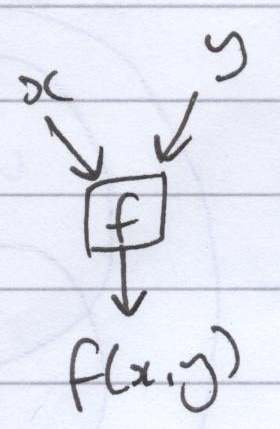
\includegraphics[width=4cm]{figs/mockups/sketches/11/11a.jpg}
\end{center}}}
\subfloat[]{
\parbox{4cm}{
\begin{center}
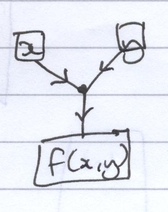
\includegraphics[width=4cm]{figs/mockups/sketches/11/11b.jpg}
\end{center}}}
\end{center}
\caption{Early designs for flowgraph-based calculation metaphors.}
\label{fig:Flows1}
% \end{wrapfigure}
\end{figure}
\end{center}

The designs in \emph{Fig.~\ref{fig:Flows1}} use a flowgraph-based metaphor, in which variables and functions are represented as nodes in the graph.  Dataflow is extremely clear in such diagrams, giving these notations high \emph{visibility}.  These designs are similar to the original one illustrated in the project proposal (\emph{Appendix D}).  The boxes and arrows used in such a metaphor also occupy relatively little screen-estate, which is advantageous in cases where a question necessitates many subcalculations.  \emph{Fig.~\ref{fig:Flows2}} shows a refined version of a flowgraph notation, with a potential environment in which to utilise it.

\begin{center}
\begin{figure}[H]
\begin{center}
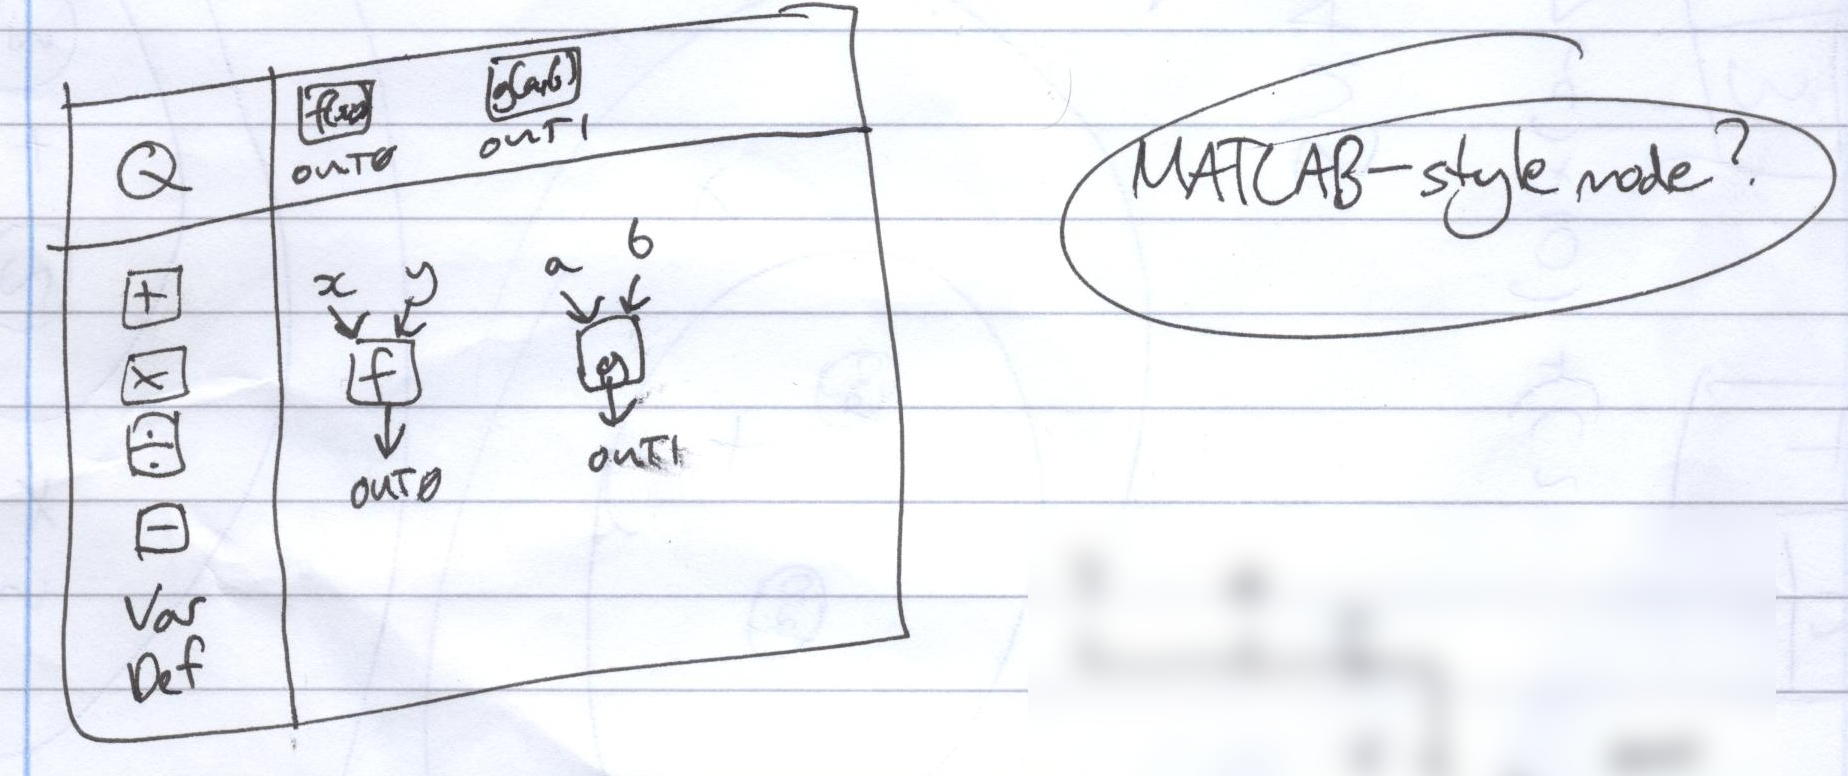
\includegraphics[width=\textwidth]{figs/mockups/sketches/11/11jii.jpg}
\end{center}
\caption{A refined sketch of a flowgraph-based language and application.}
\label{fig:Flows2}
\end{figure}
\end{center}

\begin{center}
\begin{figure}[H]
% \begin{wrapfigure}{r}{0.5\textwidth}
\begin{center}
\subfloat[]{
\parbox{4cm}{
\begin{center}
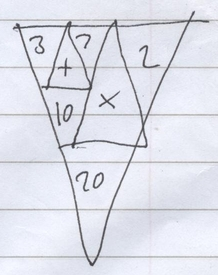
\includegraphics[width=4cm]{figs/mockups/sketches/21/21b.jpg}
\end{center}}}
\subfloat[]{
\parbox{4cm}{
\begin{center}
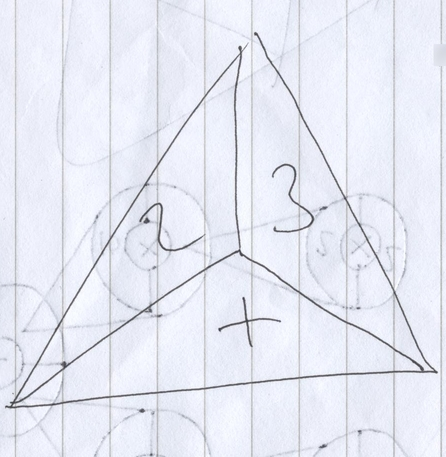
\includegraphics[width=4cm]{figs/mockups/sketches/22/22a.jpg}
\end{center}}}
\subfloat[]{
\parbox{4cm}{
\begin{center}
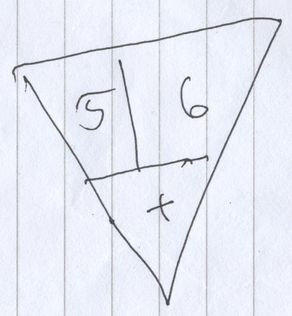
\includegraphics[width=4cm]{figs/mockups/sketches/22/22b.jpg}
\end{center}}}\\
\subfloat[]{
\parbox{4cm}{
\begin{center}
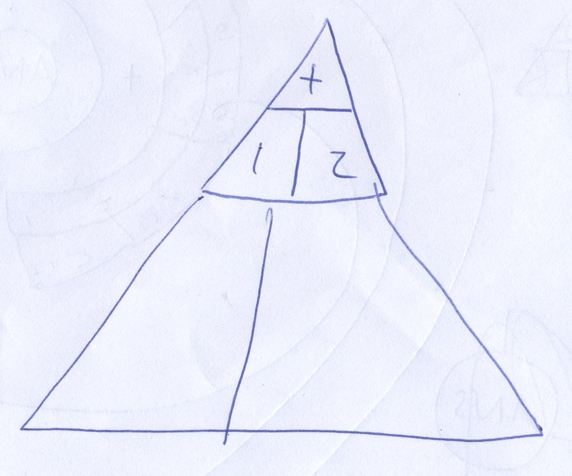
\includegraphics[width=4cm]{figs/mockups/sketches/42/42a.jpg}
\end{center}}}
\subfloat[]{
\parbox{4cm}{
\begin{center}
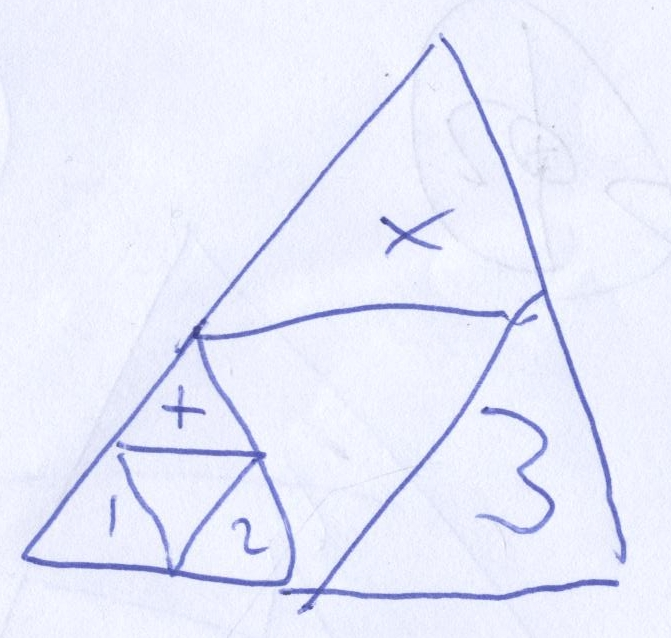
\includegraphics[width=4cm]{figs/mockups/sketches/42/42b.jpg}
\end{center}}}
\end{center}
\caption{Early designs for triangle-based calculation metaphors.}
\label{fig:Tris1}
% \end{wrapfigure}
\end{figure}
\end{center}

Triangle-based notations were also considered, drawing inspiration from the formula triangles used in science education (\emph{Fig.~\ref{fig:Tris1}}, \emph{c)} and \emph{d)}) and from the Sierpiński triangle fractal (\emph{Fig.~\ref{fig:Flows2}}, \emph{a)} and \emph{e)}).  Such notations not only appear in a form familiar to many users, but also have high \emph{visibility}.  Their \emph{juxtaposability}, however, is low, as a rigid structure is imposed upon calculations.  A more refined sketch is shown in \emph{Fig.~\ref{fig:Tris2}}.

\begin{center}
\begin{figure}
\begin{center}
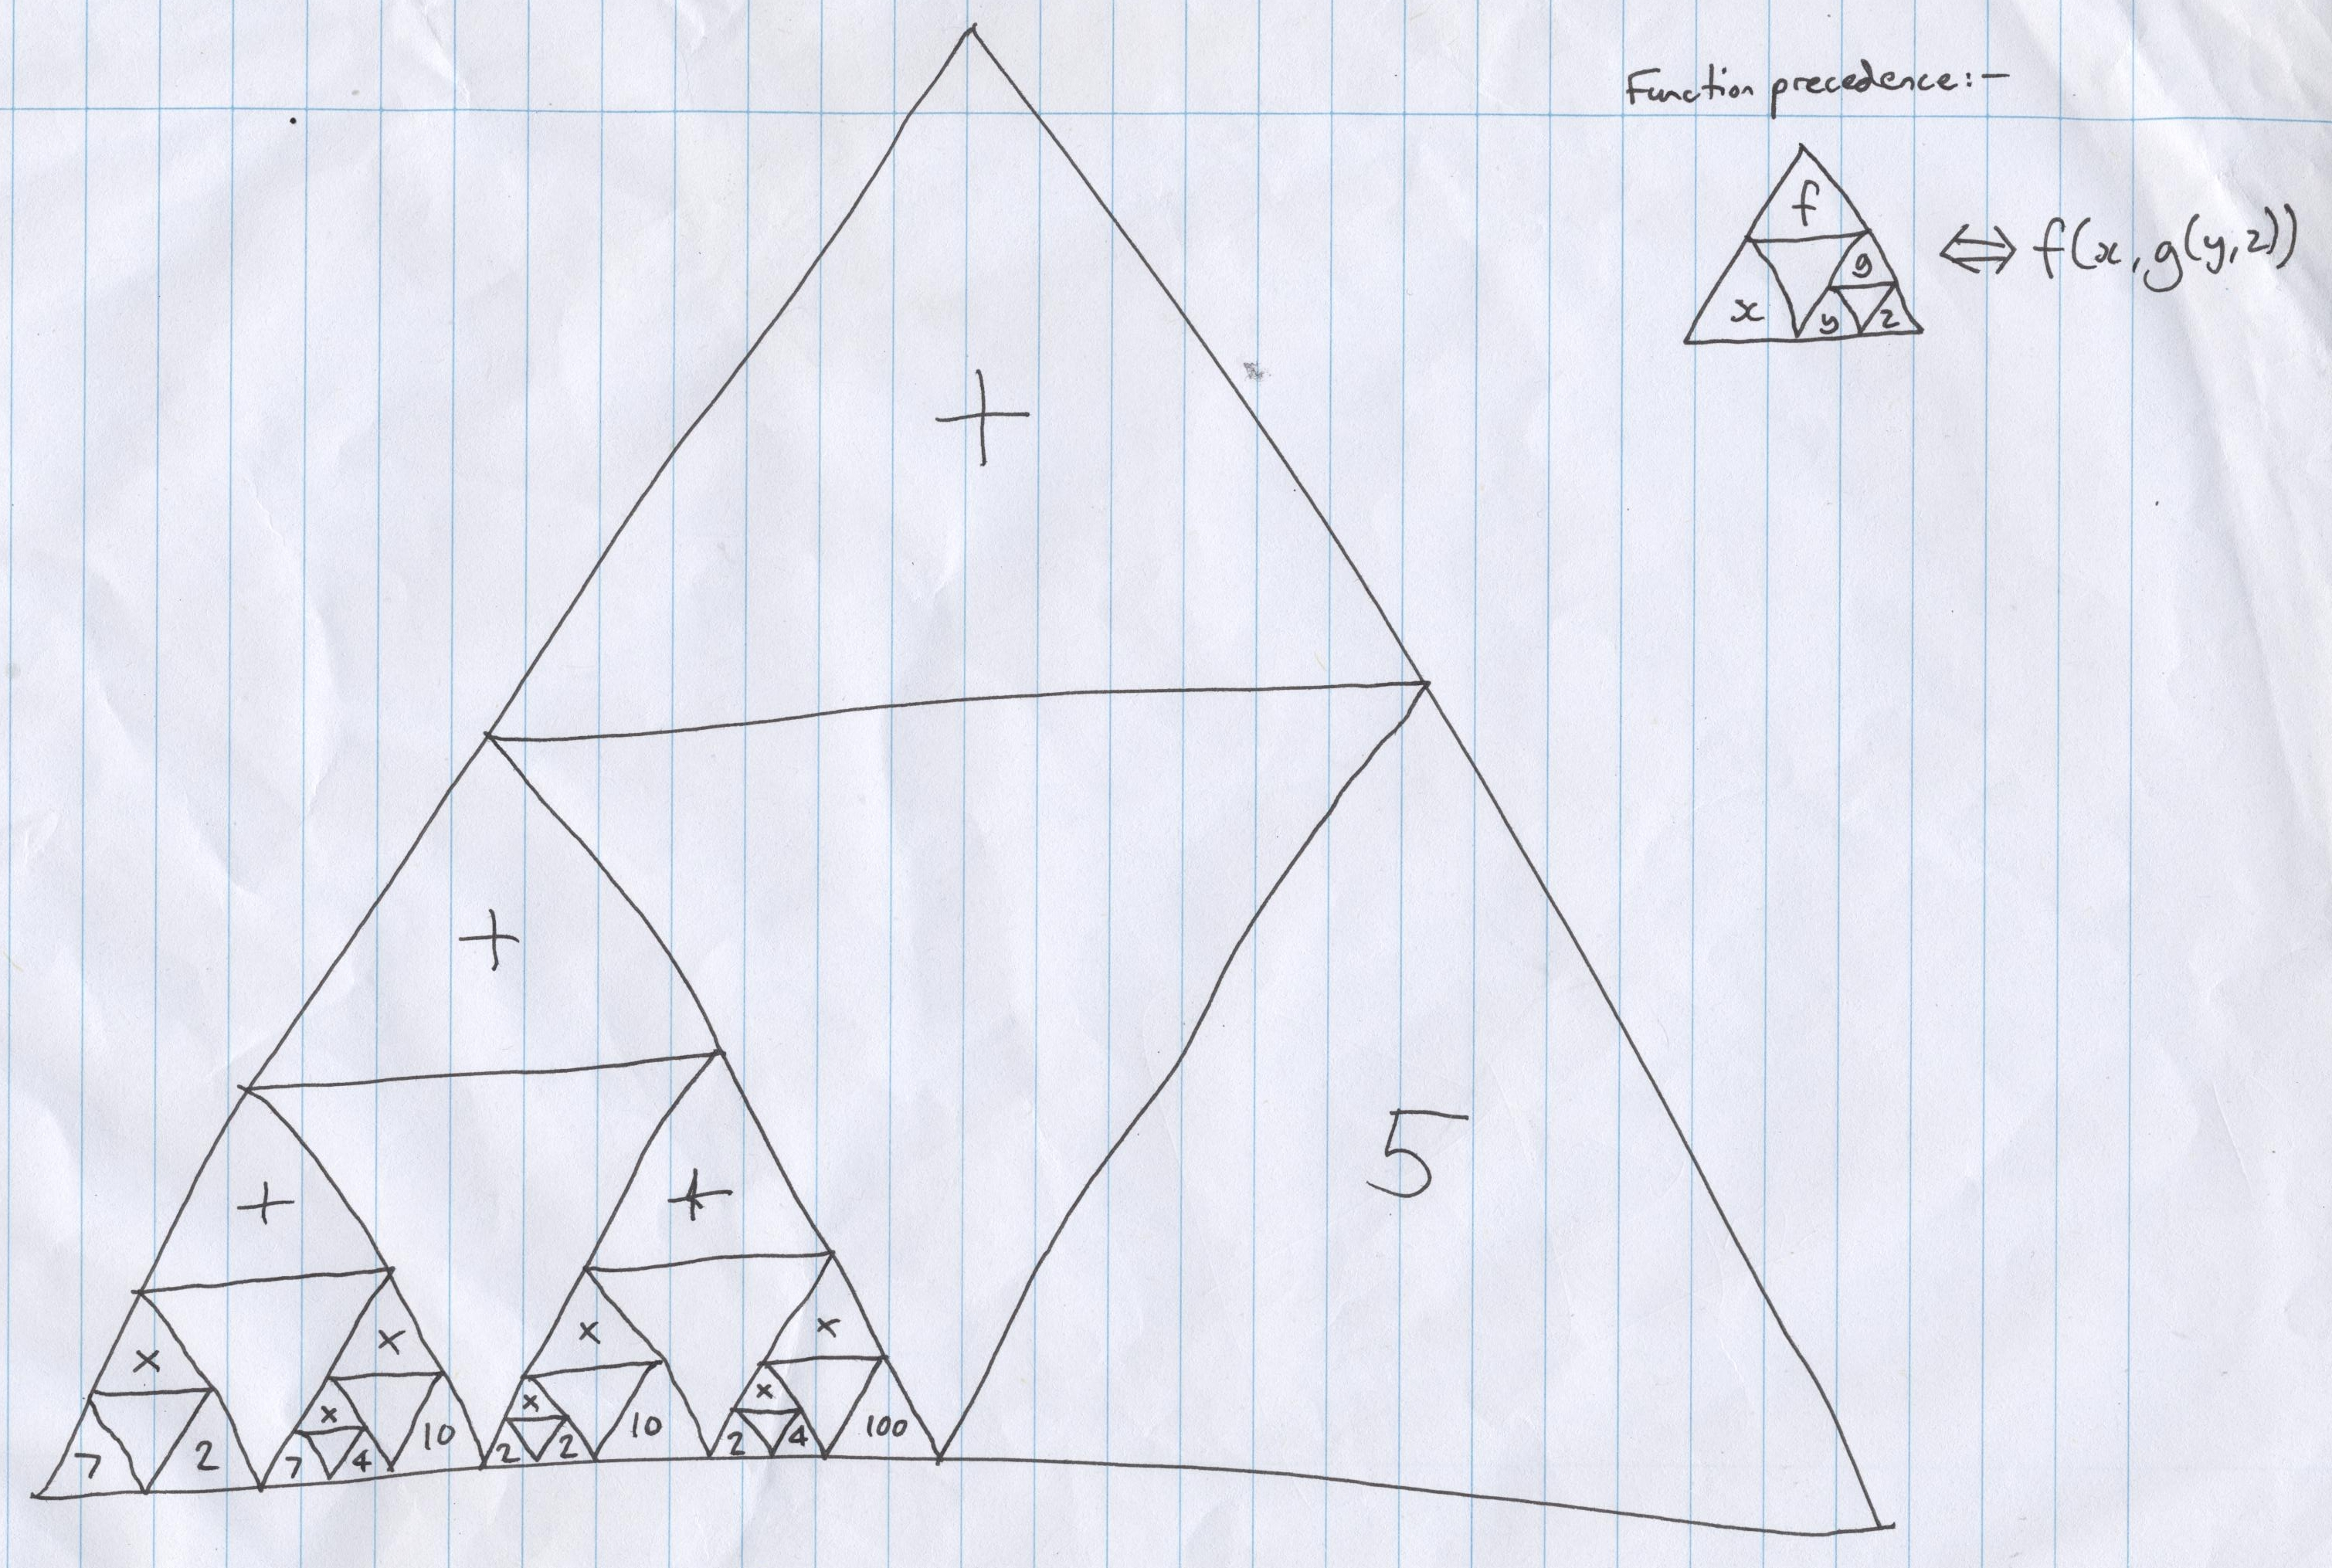
\includegraphics[width=\textwidth]{figs/mockups/sketches/31/31a.jpg}
\end{center}
\caption{A refined sketch of a triangle-based language.}
\label{fig:Tris2}
\end{figure}
\end{center}

\begin{center}
\begin{figure}[H]
% \begin{wrapfigure}{r}{0.5\textwidth}
\begin{center}
\subfloat[]{
\parbox{4cm}{
\begin{center}
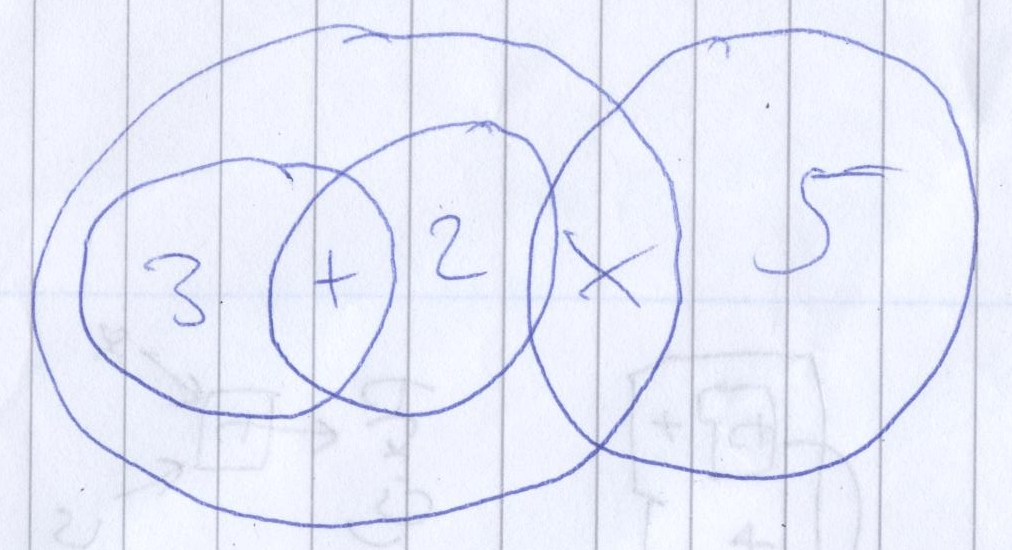
\includegraphics[width=4cm]{figs/mockups/sketches/12/12a.jpg}
\end{center}}}
\subfloat[]{
\parbox{4cm}{
\begin{center}
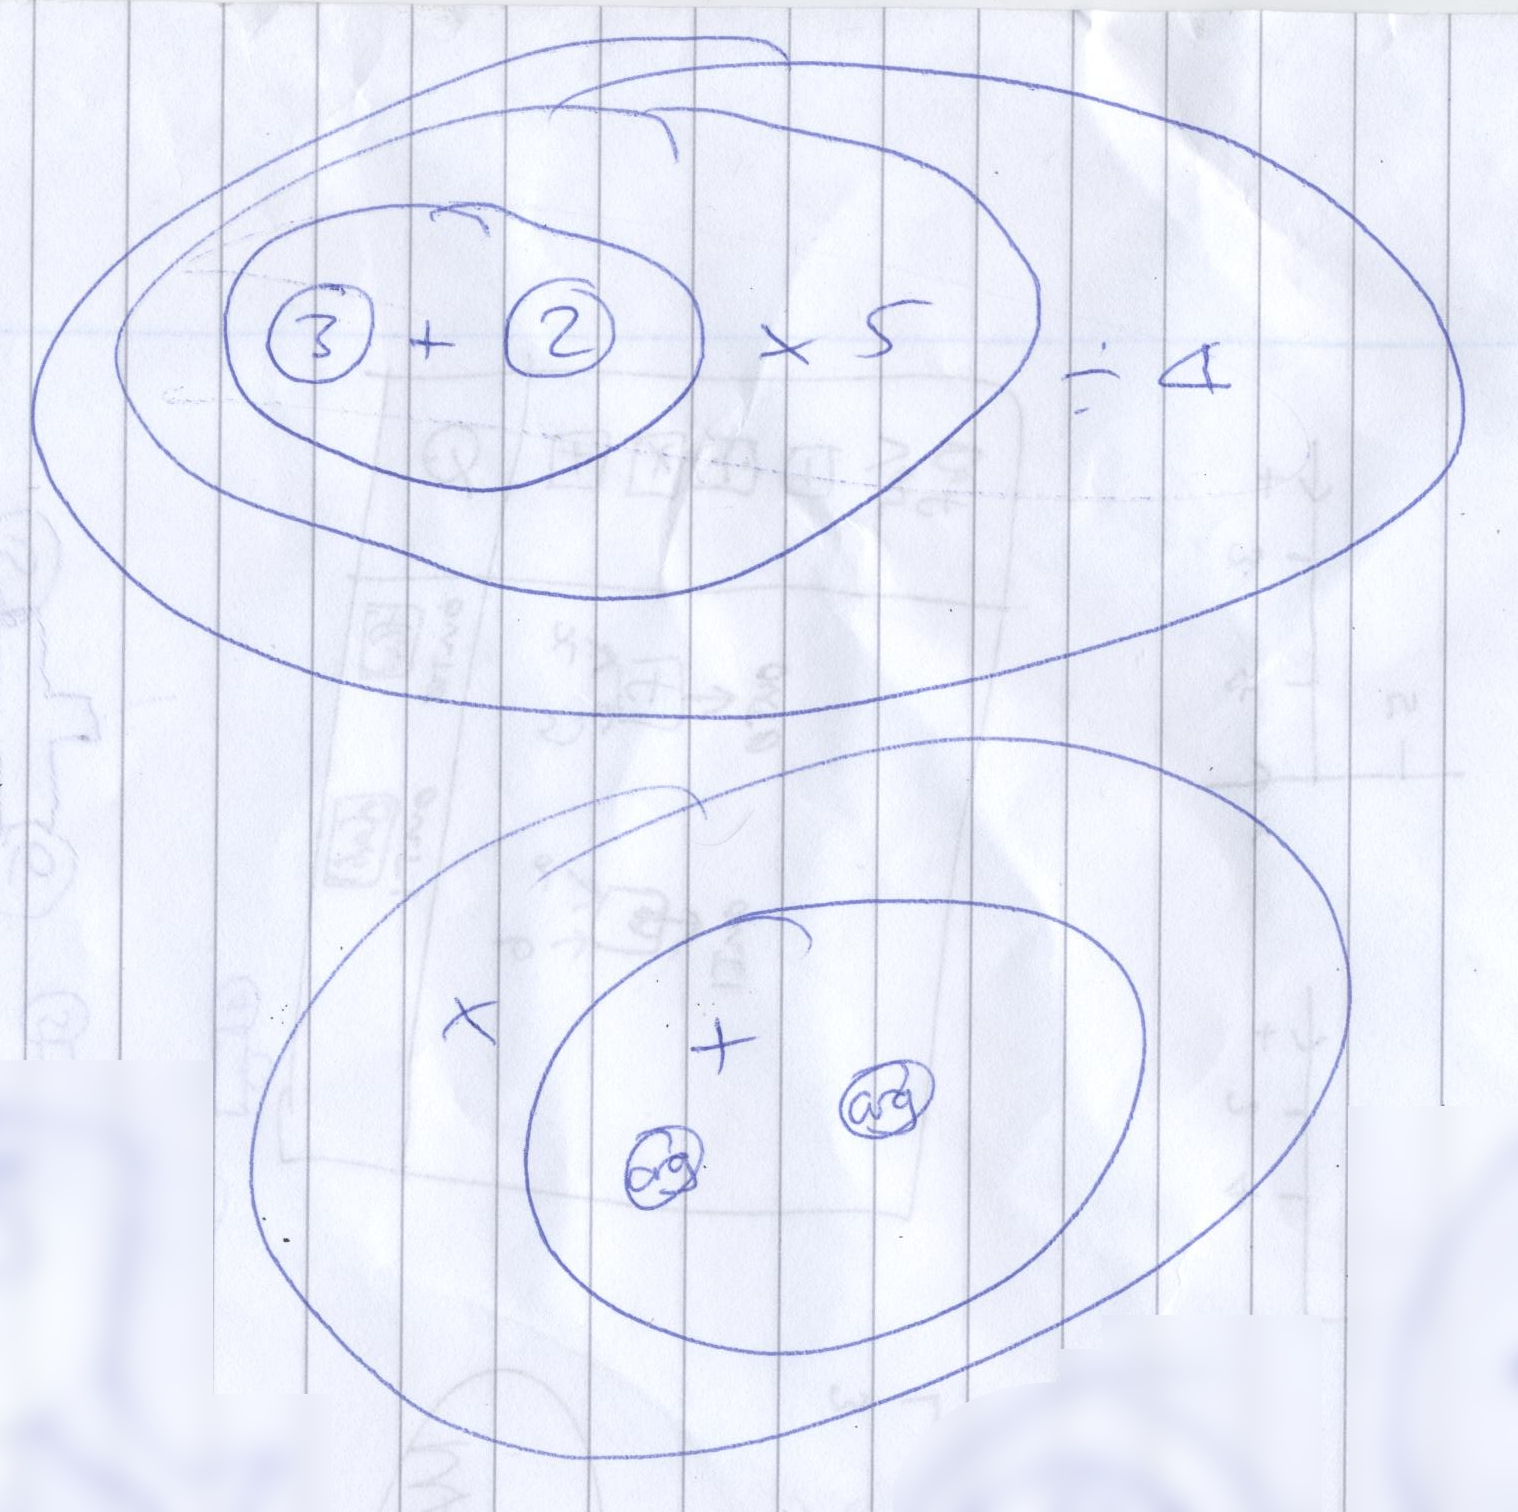
\includegraphics[width=4cm]{figs/mockups/sketches/12/12b.jpg}
\end{center}}}
\subfloat[]{
\parbox{4cm}{
\begin{center}
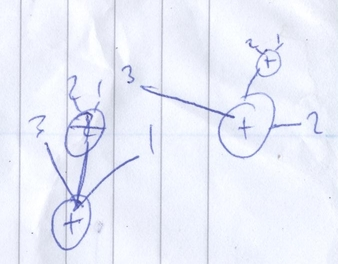
\includegraphics[width=4cm]{figs/mockups/sketches/12/12c.jpg}
\end{center}}}
\subfloat[]{
\parbox{4cm}{
\begin{center}
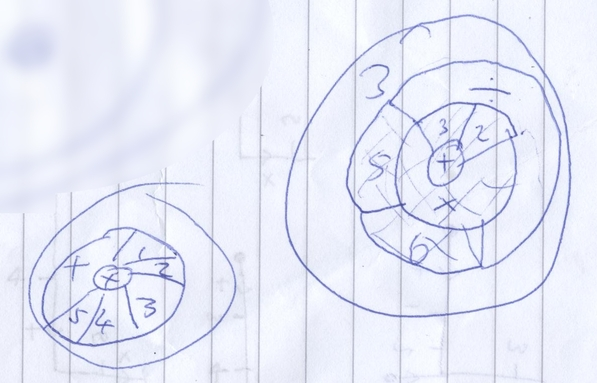
\includegraphics[width=4cm]{figs/mockups/sketches/12/12f.jpg}
\end{center}}}\\
\subfloat[]{
\parbox{4cm}{
\begin{center}
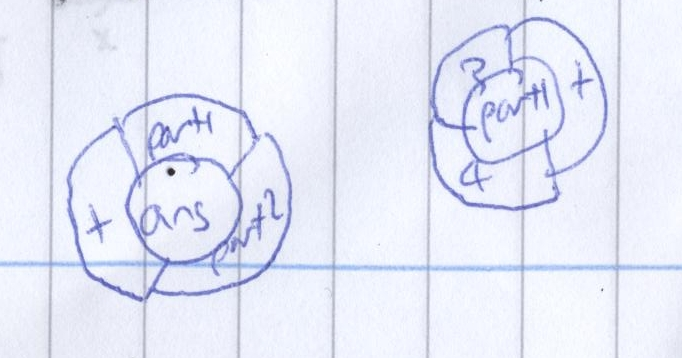
\includegraphics[width=4cm]{figs/mockups/sketches/12/12h.jpg}
\end{center}}}
\subfloat[]{
\parbox{4cm}{
\begin{center}
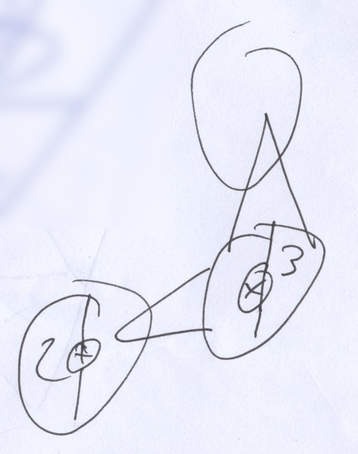
\includegraphics[width=4cm]{figs/mockups/sketches/41/41a.jpg}
\end{center}}}
\subfloat[]{
\parbox{4cm}{
\begin{center}
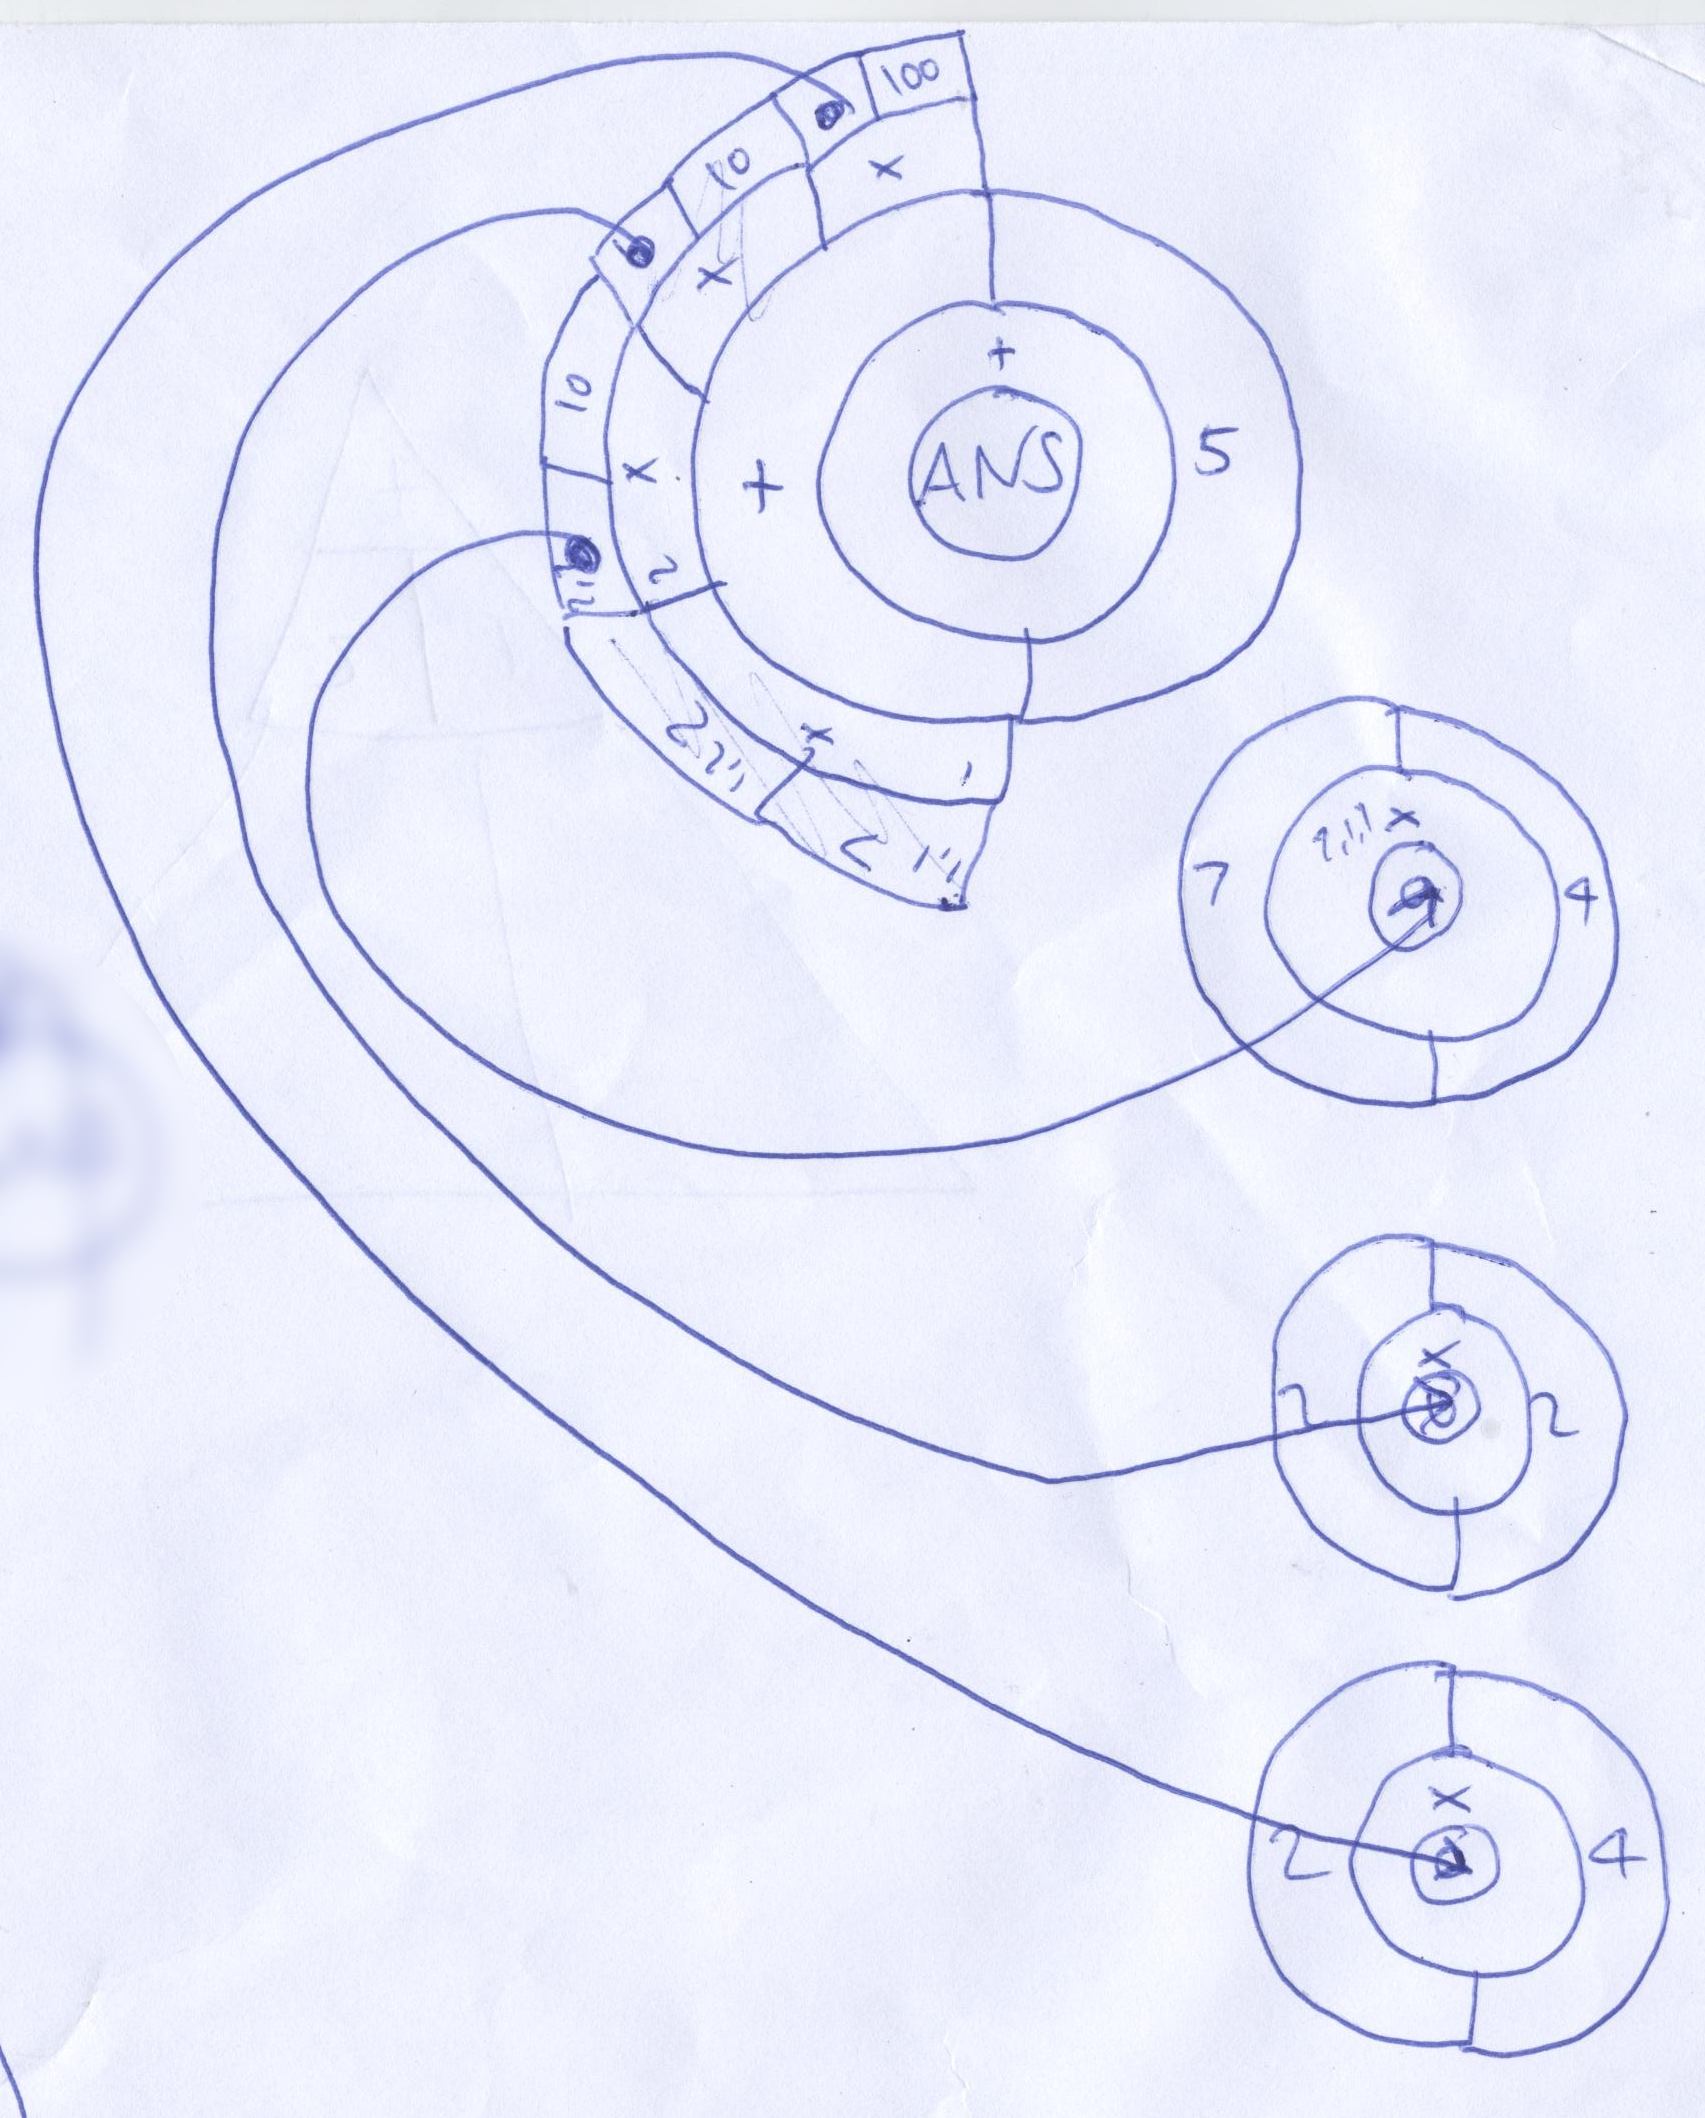
\includegraphics[width=4cm]{figs/mockups/sketches/41/41b.jpg}
\end{center}}}
\end{center}
\caption{Early designs for circle-based calculation metaphors.}
\label{fig:Circs1}
% \end{wrapfigure}
\end{figure}
\end{center}

Several circle-based notations were also considered, the focus here being on subexpressions, providing high \emph{juxtaposability}, as whole units can easily be relocated. This is opposed to using separate numbers and operations as the basic units of a large calculation.  These also offer an improvement in \emph{visibility} over handwritten arithmetic, as discussed in \emph{Sec.~2.2.1.2.3}.  A more detailed sketch is shown below.

\begin{center}
\begin{figure}[H]
\begin{center}
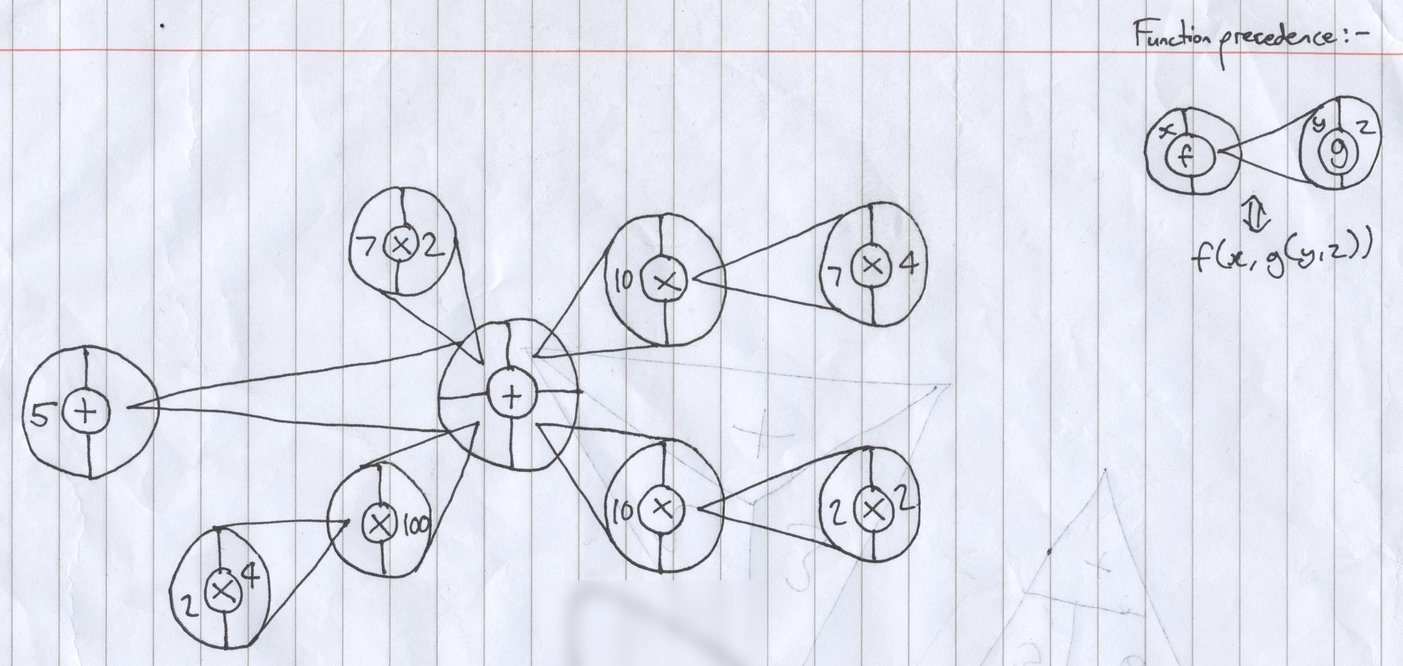
\includegraphics[width=\textwidth]{figs/mockups/sketches/21/21a.jpg}
\end{center}
\caption{A refined sketch of a circle-based language.}
\label{fig:Circs2}
\end{figure}
\end{center}

% \newpage

% \paragraph{Other}\hfill

\begin{center}
\begin{figure}[H]
% \begin{wrapfigure}{r}{0.5\textwidth}
\begin{center}
\subfloat[]{
\parbox{4cm}{
\begin{center}
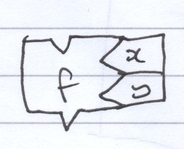
\includegraphics[width=4cm]{figs/mockups/sketches/11/11c.jpg}
\end{center}}}
\subfloat[]{
\parbox{4cm}{
\begin{center}
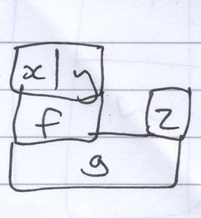
\includegraphics[width=4cm]{figs/mockups/sketches/11/11d.jpg}
\end{center}}}
\subfloat[]{
\parbox{4cm}{
\begin{center}
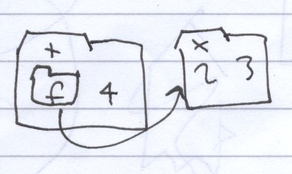
\includegraphics[width=4cm]{figs/mockups/sketches/11/11e.jpg}
\end{center}}}\\
\subfloat[]{
\parbox{4cm}{
\begin{center}
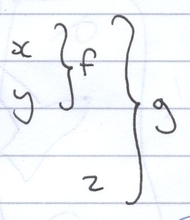
\includegraphics[width=4cm]{figs/mockups/sketches/11/11f.jpg}
\end{center}}}
\subfloat[]{
\parbox{4cm}{
\begin{center}
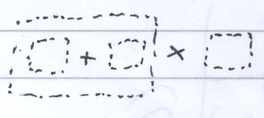
\includegraphics[width=4cm]{figs/mockups/sketches/11/11g.jpg}
\end{center}}}
\subfloat[]{
\parbox{4cm}{
\begin{center}
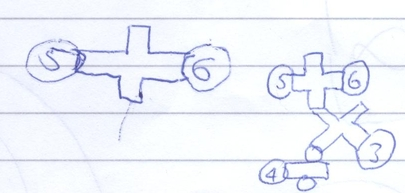
\includegraphics[width=4cm]{figs/mockups/sketches/11/11h.jpg}
\end{center}}}\\
%\end{center}
%\end{figure}
%\newpage
%\begin{figure}
%\ContinuedFloat
%\begin{center}
\subfloat[]{
\parbox{4cm}{
\begin{center}
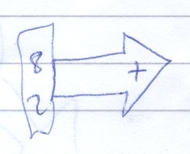
\includegraphics[width=4cm]{figs/mockups/sketches/11/11i.jpg}
\end{center}}}
\subfloat[]{
\parbox{4cm}{
\begin{center}
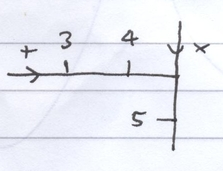
\includegraphics[width=4cm]{figs/mockups/sketches/11/11k.jpg}
\end{center}}}
\subfloat[]{
\parbox{4cm}{
\begin{center}
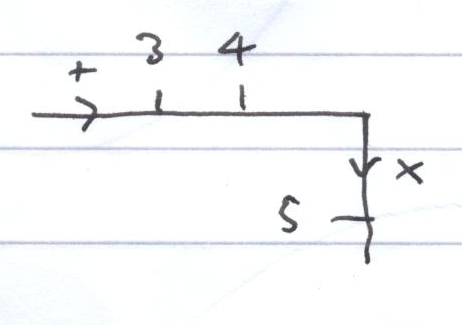
\includegraphics[width=4cm]{figs/mockups/sketches/11/11li.jpg}
\end{center}}}\\
\subfloat[]{
\parbox{4cm}{
\begin{center}
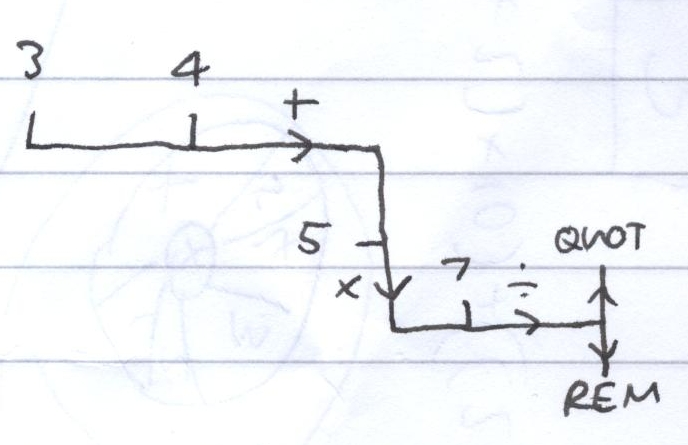
\includegraphics[width=4cm]{figs/mockups/sketches/11/11lii.jpg}
\end{center}}}
\subfloat[]{
\parbox{4cm}{
\begin{center}
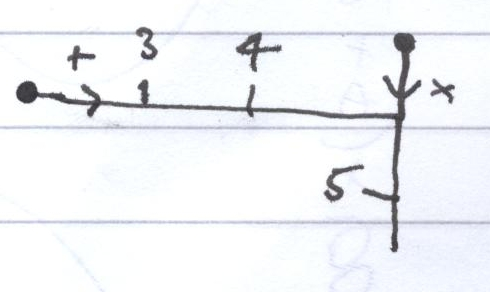
\includegraphics[width=4cm]{figs/mockups/sketches/11/11m.jpg}
\end{center}}}
\subfloat[]{
\parbox{4cm}{
\begin{center}
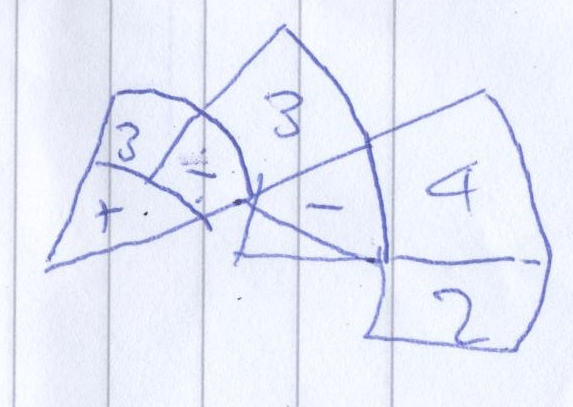
\includegraphics[width=4cm]{figs/mockups/sketches/12/12d.jpg}
\end{center}}}\\
\subfloat[]{
\parbox{4cm}{
\begin{center}
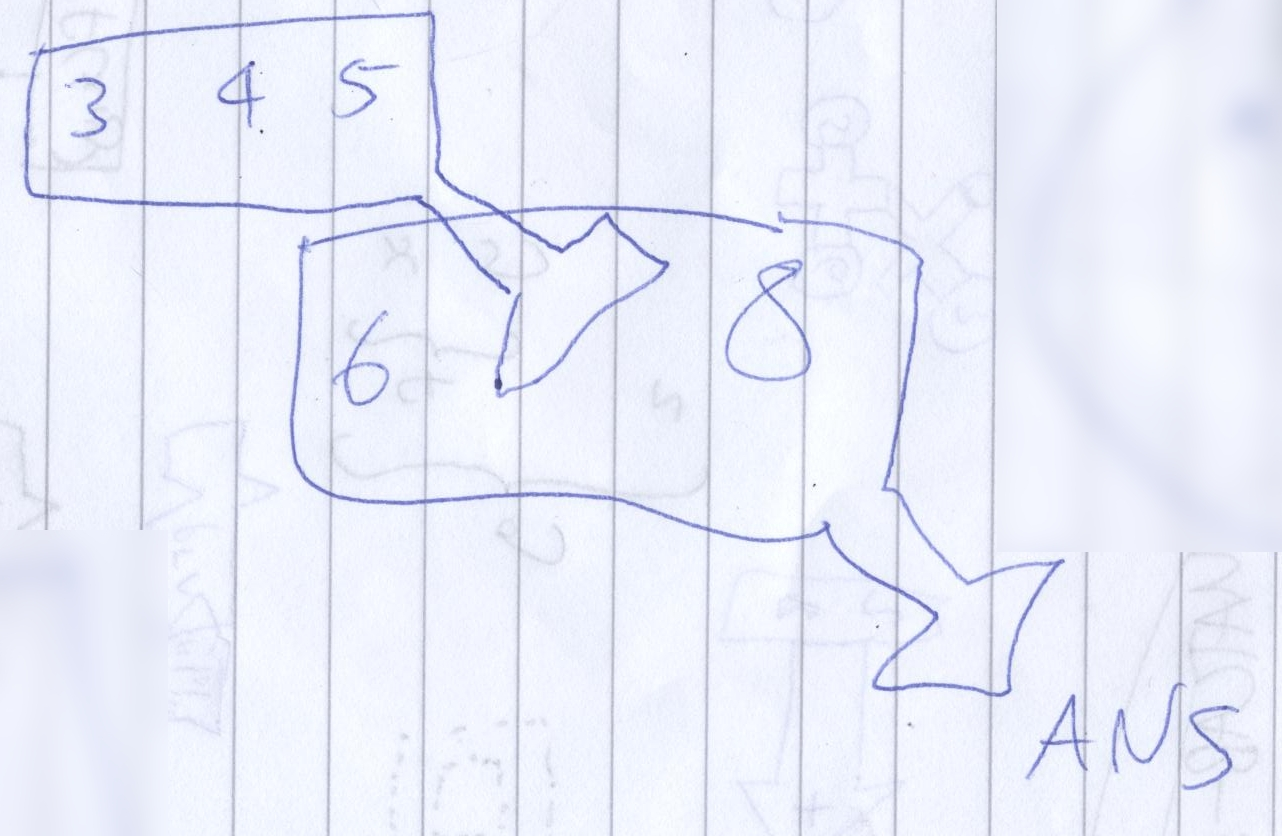
\includegraphics[width=4cm]{figs/mockups/sketches/12/12e.jpg}
\end{center}}}
\end{center}
\caption{Assorted early designs for other calculation metaphors.}
\label{fig:Others1}
% \end{wrapfigure}
\end{figure}
\end{center}

\begin{center}
\begin{figure}[H]
\begin{center}
\subfloat[]{
\parbox{4cm}{
\begin{center}
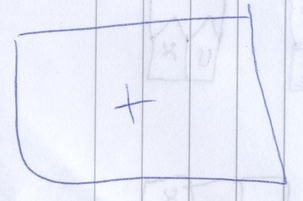
\includegraphics[width=4cm]{figs/mockups/sketches/12/12gi.jpg}
\end{center}}}
{\Huge $ \rightarrow $}% arrow
\subfloat[]{
\parbox{4cm}{
\begin{center}
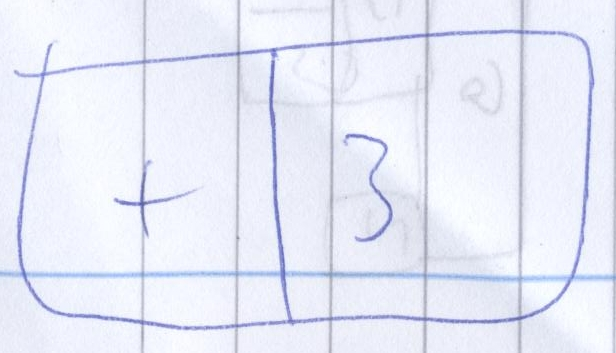
\includegraphics[width=4cm]{figs/mockups/sketches/12/12gii.jpg}
\end{center}}}
{\Huge $ \rightarrow $}\\% arrow
\subfloat[]{
\parbox{4cm}{
\begin{center}
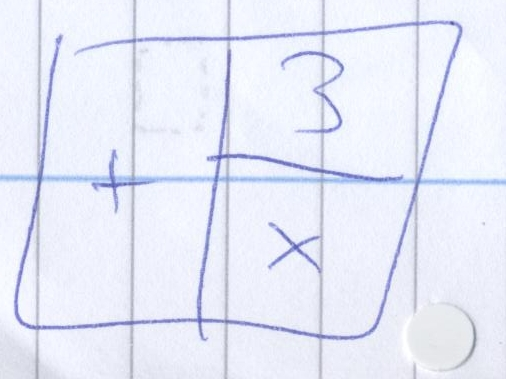
\includegraphics[width=4cm]{figs/mockups/sketches/12/12giii.jpg}
\end{center}}}
{\Huge $ \rightarrow $}% arrow
\subfloat[]{
\parbox{4cm}{
\begin{center}
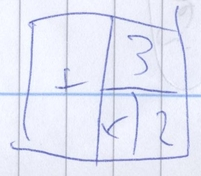
\includegraphics[width=4cm]{figs/mockups/sketches/12/12giv.jpg}
\end{center}}}
{\Huge $ \rightarrow $}% arrow
\subfloat[]{
\parbox{4cm}{
\begin{center}
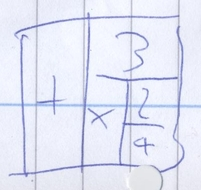
\includegraphics[width=4cm]{figs/mockups/sketches/12/12gv.jpg}
\end{center}}}
\end{center}
\caption{A sample progression of a calculation using a language based around an infinitely-subdivided rectangle.}
\label{fig:Others2}
\end{figure}
\end{center}

Various other metaphors for calculation were also considered, as illustrated in \emph{Figs.~\ref{fig:Others1} and \ref{fig:Others2}}.  \emph{Fig.~\ref{fig:Others1} a)} was considered too similar to Google/MIT's \emph{App Inventor} software.  Sketches \emph{c)}, \emph{f)}, \emph{l)} and \emph{m)} were deemed too cumbersome, and \emph{d)}, \emph{e)} and \emph{h)} to \emph{k)} were not considered visually appealing, appearing too similar to existing mathematical notations and constructs.  Items \emph{b)} and \emph{g)} were inflexible, and would have scaled poorly to larger calculations.  Finally \emph{Fig.~\ref{fig:Others2}} was rejected as it was too similar to the Sierpiński triangle metaphor shown in \emph{Fig.~\ref{fig:Tris2}}.

\subsubsection{Detailed Mockups}
% examples done using that prototyping software - balsamiq mockups
% draft designs on pwf

More mature designs for the application and graphical language follow.  First is a combined flowgraph representation and Read-Evaluate-Print-Loop (REPL) design.  The second uses the Sierpiński triangle as a basis for the visual metaphor.  The final design is a circle-based language, similar to \emph{Fig.~\ref{fig:Circs2}}.

% TODO: these fuckers
\paragraph{Flowgraph Metaphor}\hfill

\begin{figure}[H]
\begin{center}
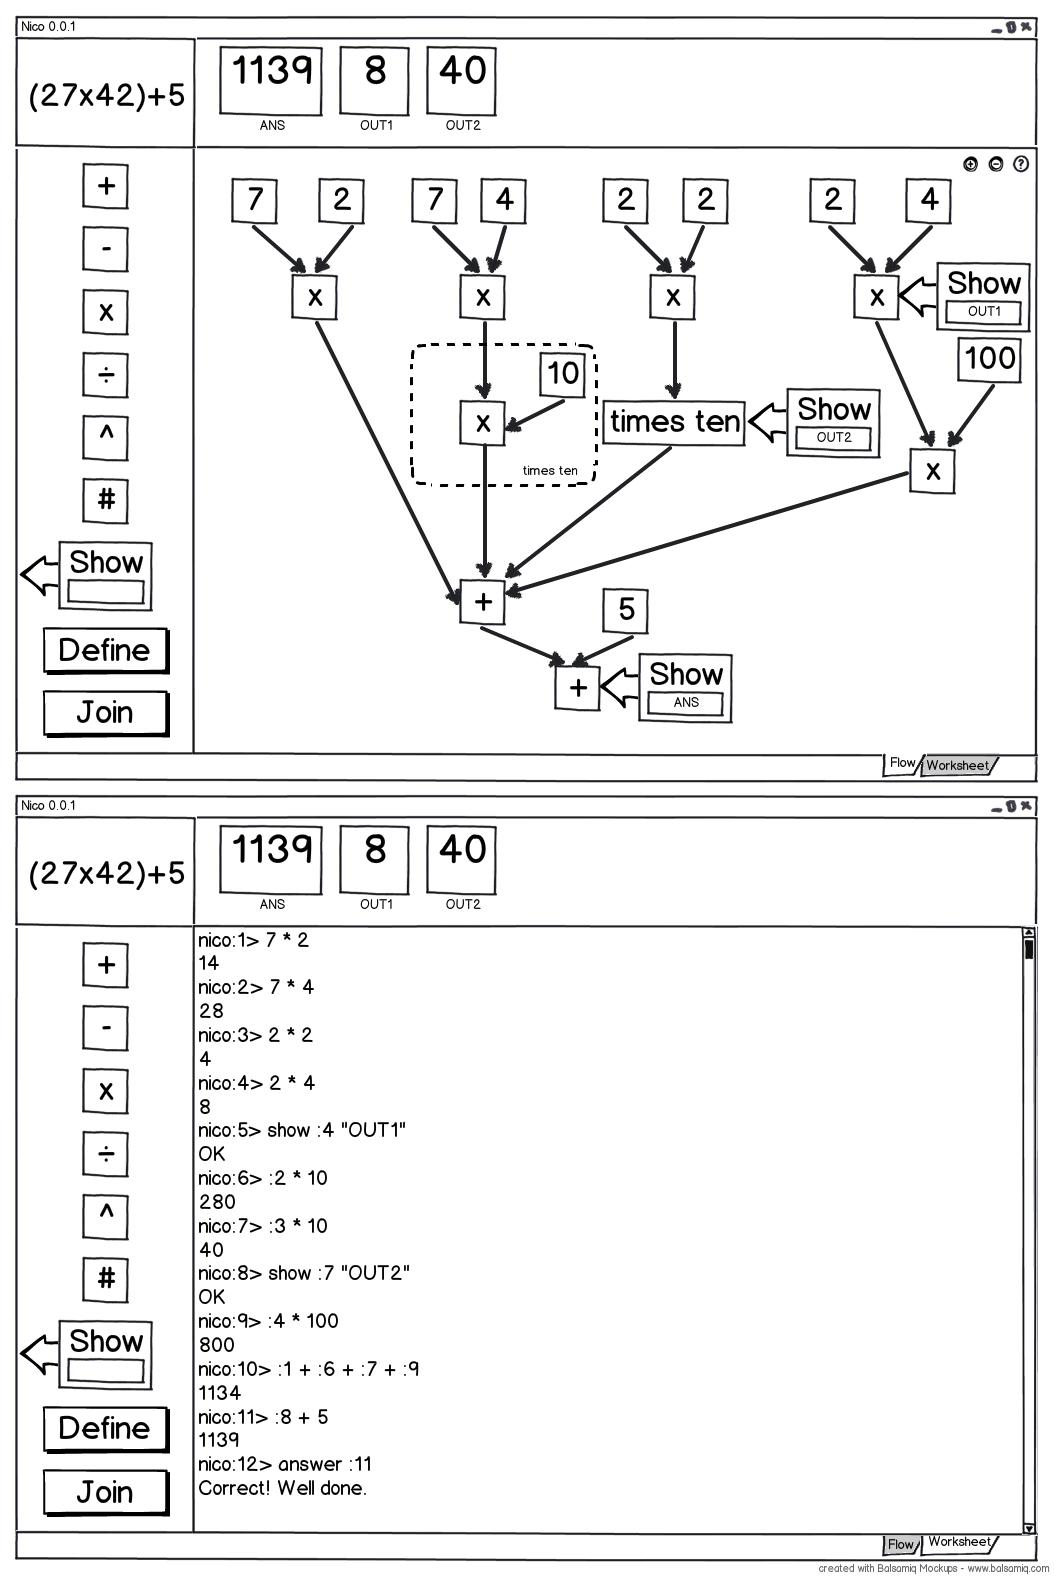
\includegraphics[width=\textwidth-4cm]{figs/mockups/flowgraph/img/fg-000.jpg}
\caption{The prototype flowgraph-style language and accompanying application.}
\label{fig:ProtoFlow}
\end{center}
\end{figure}

This layout expands the application prototyped in the project proposal.  The application now comprises one window containing information panels, a `toolbox' of available functions that can be dragged on to the canvas, and a canvas area upon which calculations are constructed.  Zoom and help buttons are provided.  The user is able to use the {\sfapp Flow} and {\sfapp Worksheet} tabs to switch between the graphical mode and the REPL mode respectively.

The top screen in \emph{Fig.~\ref{fig:ProtoFlow}} shows manipulation of the graphical language, whilst the bottom screen shows a REPL utilising a simple text-based language.  The flowgraph notation was used as it is \emph{visible}, making the flow of data very clear to the user and allowing them to see much of their structure at once.  The notation also occupies little screen-estate, allowing it to accommodate large calculations.

The toolbox was included to exhibit available functions.  In the original design, no control scheme was specified; the user was expected to have control over many different functions, meaning that unless it were simple, the user may require guidance.  There are two buttons in the toolbox: {\sfapp Join}, which changes the function of the mouse to join boxes with arrows; and {\sfapp Define}, which similarly allows the user to draw a box around a subsection of the diagram to define a function.  This was introduced to allow for the creation of abstractions for repeated tasks, making the language more compact.  It was decided to use these modes, combined with the placement of boxes in the default mode, so that the entire control scheme could be implemented using one mouse button.

The zoom buttons were included to accommodate large diagrams, and to allow the user to view their work at a comfortable size.  The help button was included to provide assistance for new users.  Activating help would provide information explaining how the application works.

The {\sfapp Worksheet} mode was included for users who may feel more comfortable working in a written environment, rather than using the graphical metaphor.

This design was abandoned as it was deemed to be too complex for the target audience (Year 5).  The intention of this project was not to implement an educational programming language, and by including functionality such as the REPL and {\sfapp Define}, the system overprovides.  The REPL itself is superfluous, as users comfortable working in a textual environment are likely to be comfortable using the handwritten method.

In addition to this, the flowgraph representation had a number of more general shortcomings. For example, the evaluation order of arguments is unclear, which is confusing for non-commutative functions such as subtraction.  Furthermore, the language is verbose.  This is not inherently a disadvantage but a more compact representation would be preferable in order to make expressions more \emph{visible}, and to decrease time spent by the user searching for information within the notation.  It is also \emph{viscous} when replacing whole subcalculations, rather than just numbers or operators, though less so than handwritten arithmetic.

\paragraph{Sierpiński Triangle Metaphor}\hfill

\begin{figure}[H]
\begin{center}
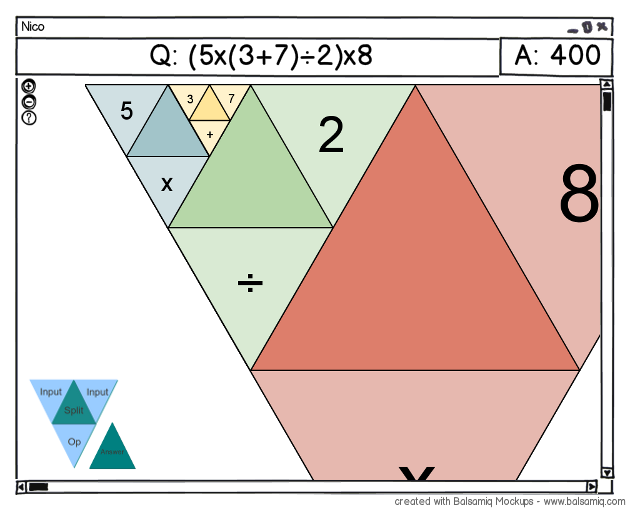
\includegraphics[width=\textwidth]{figs/mockups/sierp/sierp_mockup_full.png}
\caption{The prototype Sierpiński-triangle-based language and accompanying application.}
\label{fig:ProtoTri}
\end{center}
\end{figure}

This prototype uses a zooming instance of the Sierpiński triangle fractal as the basis of its notation, as shown in \emph{Fig.~\ref{fig:ProtoTri}.  The application consists of a single window with information panels and a canvas area, featuring zoom and help buttons, as well as control buttons for diagram construction.

This prototype marks a significant departure from the flowgraph metaphor outlined above and in the project proposal to address the above problems with the flowgraph notation.  The application also had to change to suit the new notation: in this case, a toolbox would not be suitable, as the user is limited to one structure.

The triangle notation was chosen as it is more \emph{visible} than the handwritten method, and places considerable emphasis on structure, making it clear how smaller calculations can combine to form larger ones by using a fractal-based notation.  It is colour-coded by the level of nesting of each triangle, clarifying at which level the user is working and allowing the user to abstract away smaller triangles as arguments to encompassing calculations.

Zoom buttons were included as, although the size of the overall structure always remains the same in this notation, it becomes necessary to read very small sections quite quickly, as nested calculations are built up.  Indeed, each section constitutes a quarter of the area of the triangle that contains it, as illustrated in \emph{Fig.~\ref{fig:ProtoTri}}.

As in the previous prototype, a help button was included to ease initiation.

A control scheme using buttons was again chosen so that only one mouse-button was required.  The arrangement of the control buttons maps to the arrangement of triangles within the diagram.  This design was chosen to clarify the consequences of each control upon the structure: the {\sfapp Input} and {\sfapp Op} buttons allow the user to modify the corresponding section of the triangle.  The user is able to submit answers using the {\sfapp Answer} button, allowing them to check and change their solutions before submission.

This design was ultimately abandoned as it was awkward. It is based around binary operations, meaning that to solve the simple question 1+2+3+4, one has to either calculate ((1+2)+3)+4, which is inefficient; or deduce that 1+2+3=6 and then calculate 6+4, which is unacceptable for a system designed to aid arithmetic learning.

The severe lack of \emph{juxtaposability} is also problematic: as each expression must fit into the larger structure, it is not possible to reorder them without fundamentally altering the calculation being performed.  It also enforces a top-down approach to calculation: one is required to begin with the outermost calculation and work inwards.  There is no provision for encapsulating an existing calculation within another triangle without significant \emph{premature commitment}.

In addition to this, an informal survey regarding potential notations was conducted, asking approximately ten participants to answer some sample questions in this notation and the circle-based notation below.  Participants found this notation less clear, and were able to complete more questions correctly using the circle notation.
% survey
% TODO: can't put subexpressions into right-hand triangle

% what/mockup
% application
% language
% abandoned

\paragraph{Circle Metaphor}\hfill

\begin{figure}[H]
\begin{center}
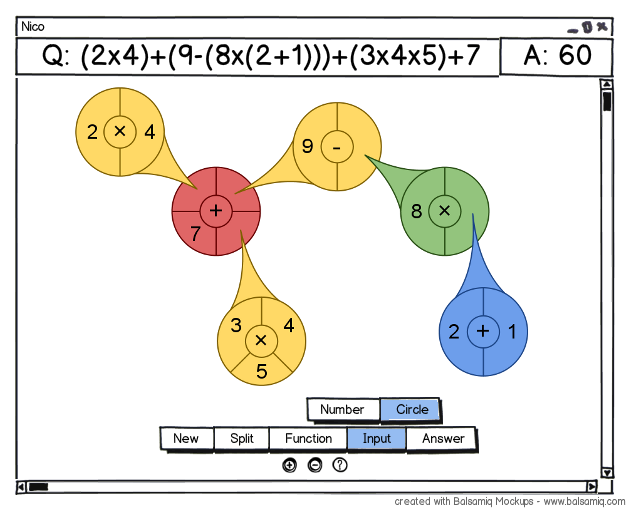
\includegraphics[width=\textwidth]{figs/mockups/circles/nico_circmock.png}
\caption{The prototype circle-based language and accompanying application.}
\label{fig:ProtoCirc}
\end{center}
\end{figure}

In this prototype, circles constitute individual units of calculation, linked to indicate the flow of information. Each circle consists of an operator, around which arguments orbit, which are evaluated clockwise from 0°.  It is related to the flowgraph metaphor above, but has a number of key differences.

The application comprises a single window with information panels and a canvas, which includes control, zoom and help buttons, similar to the previous two models.  Zoom buttons accomodate large diagrams, again allowing the user to focus on small sections and to work at a scale that is comfortable.  The help button eases initiation.

Similar to the {\sfapp Define} and {\sfapp Join} buttons in \emph{Fig.~\ref{fig:ProtoFlow}}, the buttons specify mouse modes: {\sfapp New} causes clicking to create new circles, {\sfapp Split} causes clicked circles to gain an argument, and so on. The motivations for this were similar to that for the modes in the flowgraph model, including the ability to control the software using one mouse button.  The user is able to submit answers using the {\sfapp Answer} button, to allow them to check and change their answers before submission.

Again, this prototype is markedly different to the idea originally proposed.  The application has changed to accommodate the new notation: a toolbox is unsuitable as the notation uses only one fundamental structure, a circle, and the controls in the Sierpiński model (\emph{Fig.~\ref{fig:ProtoTri}}) are inappropriate.

Unlike the Sierpiński metaphor, the user is not restricted to one order or pattern of constructing a calculation.  The circle `tails' make the flow of information through the diagram clear, and are colour-coded by their level of nesting, to further clarify dataflow and to eliminate \emph{hidden dependencies}.

The circle metaphor was chosen for similar reasons to the triangle model: it emphasises the idea of subcalculations as individual units to be abstracted away and treated as any other argument.  This notation has greater \emph{visibility} than handwritten arithmetic, and offers more flexibility than the previous two models, decreasing \emph{viscosity} by allowing the user to edit whole expressions within a calculation and exchange them as needed.  \emph{Juxtaposability} is increased as whole subcalculations are easily repositioned.  The system requires little \emph{premature commitment}, as any piece of the diagram can be modified at will.  This is ideal for exploration, allowing the user to try many ways of solving a problem within the application, rather than having to use a secondary notation or device to help work through a problem and transcribing the result.

This design was ultimately chosen as it solved, or at least ameliorated, many of the problems listed with handwritten arithmetic, without being too complex for the target audience, and without being too restrictive with regard to mathematical expression.  Furthermore, the results of the survey mentioned above also indicated that participants found this notation more intuitive, and made fewer mistakes.

% what/mockup
% application
% language
% chosen

% \section{Additional Tools}

% Luke's:
% Throughout the project, I developed additional support tools to assist with
% design, development and testing. These will be described at the relevant place
% in the implementation chapter.
% lol

\section{Summary}

Prior to the implementation of the project, a thorough requirements analysis was conducted to outline the expected behaviour of the application, contrasting it with the existing system of handwritten calculations.  In \emph{Sec.~2.2}, prototypes for a suitable graphical notation were developed, and three were explored in detail.  Two of these were offered as alternatives to the flawed original design.  The final choice of the circle-based metaphor has many advantanges over the original flowgraph notation.

\cleardoublepage
\chapter{Implementation}

This chapter includes a discussion of the system architecture, detailing the implementation of its infrastructure, management of mutable state, administration of circles, interpretation and evaluation of the notation, and handling of the questions posed to the user.  This is followed by a discussion of the interaction handler, the libraries used, the underlying structure of the user interface and the control scheme.  Next, there is an analysis of the development of the user interface, considering the application itself and its control scheme, use of colour-coding and notation.  Finally there is a discussion of testing methods used.

The code itself totals approximately 1,500 lines of Clojure, and the application satisfies the success criteria in the project proposal, namely:
\begin{center}
\parbox[c]{\textwidth-2cm}{
\small
``[to be] able to generate an abstract syntax tree in Clojure from the graphical language and evaluate such a tree, passing the results back to the graphical application and displaying this to user in less than 300ms.''
}
\end{center}
In addition to this, an extension to the project was completed, in the form of a user study.

\section{System Architecture}
% TODO: intro?

The system comprises three layers of operation: the user interface, the interaction handler and the infrastructure.  Events occurring in the user interface are processed by the interaction handler, with the resultant data being passed to the infrastructure.  This handles the interpretation of such data, as well as the memory-management operations.  Data can also flow from the infrastructure to the interaction handler, with results being passed to the interaction handler, causing effects in the user interface.  A detailed analysis of each layer follows.

\begin{landscape}
\begin{center}
\begin{figure}[H]
\begin{center}
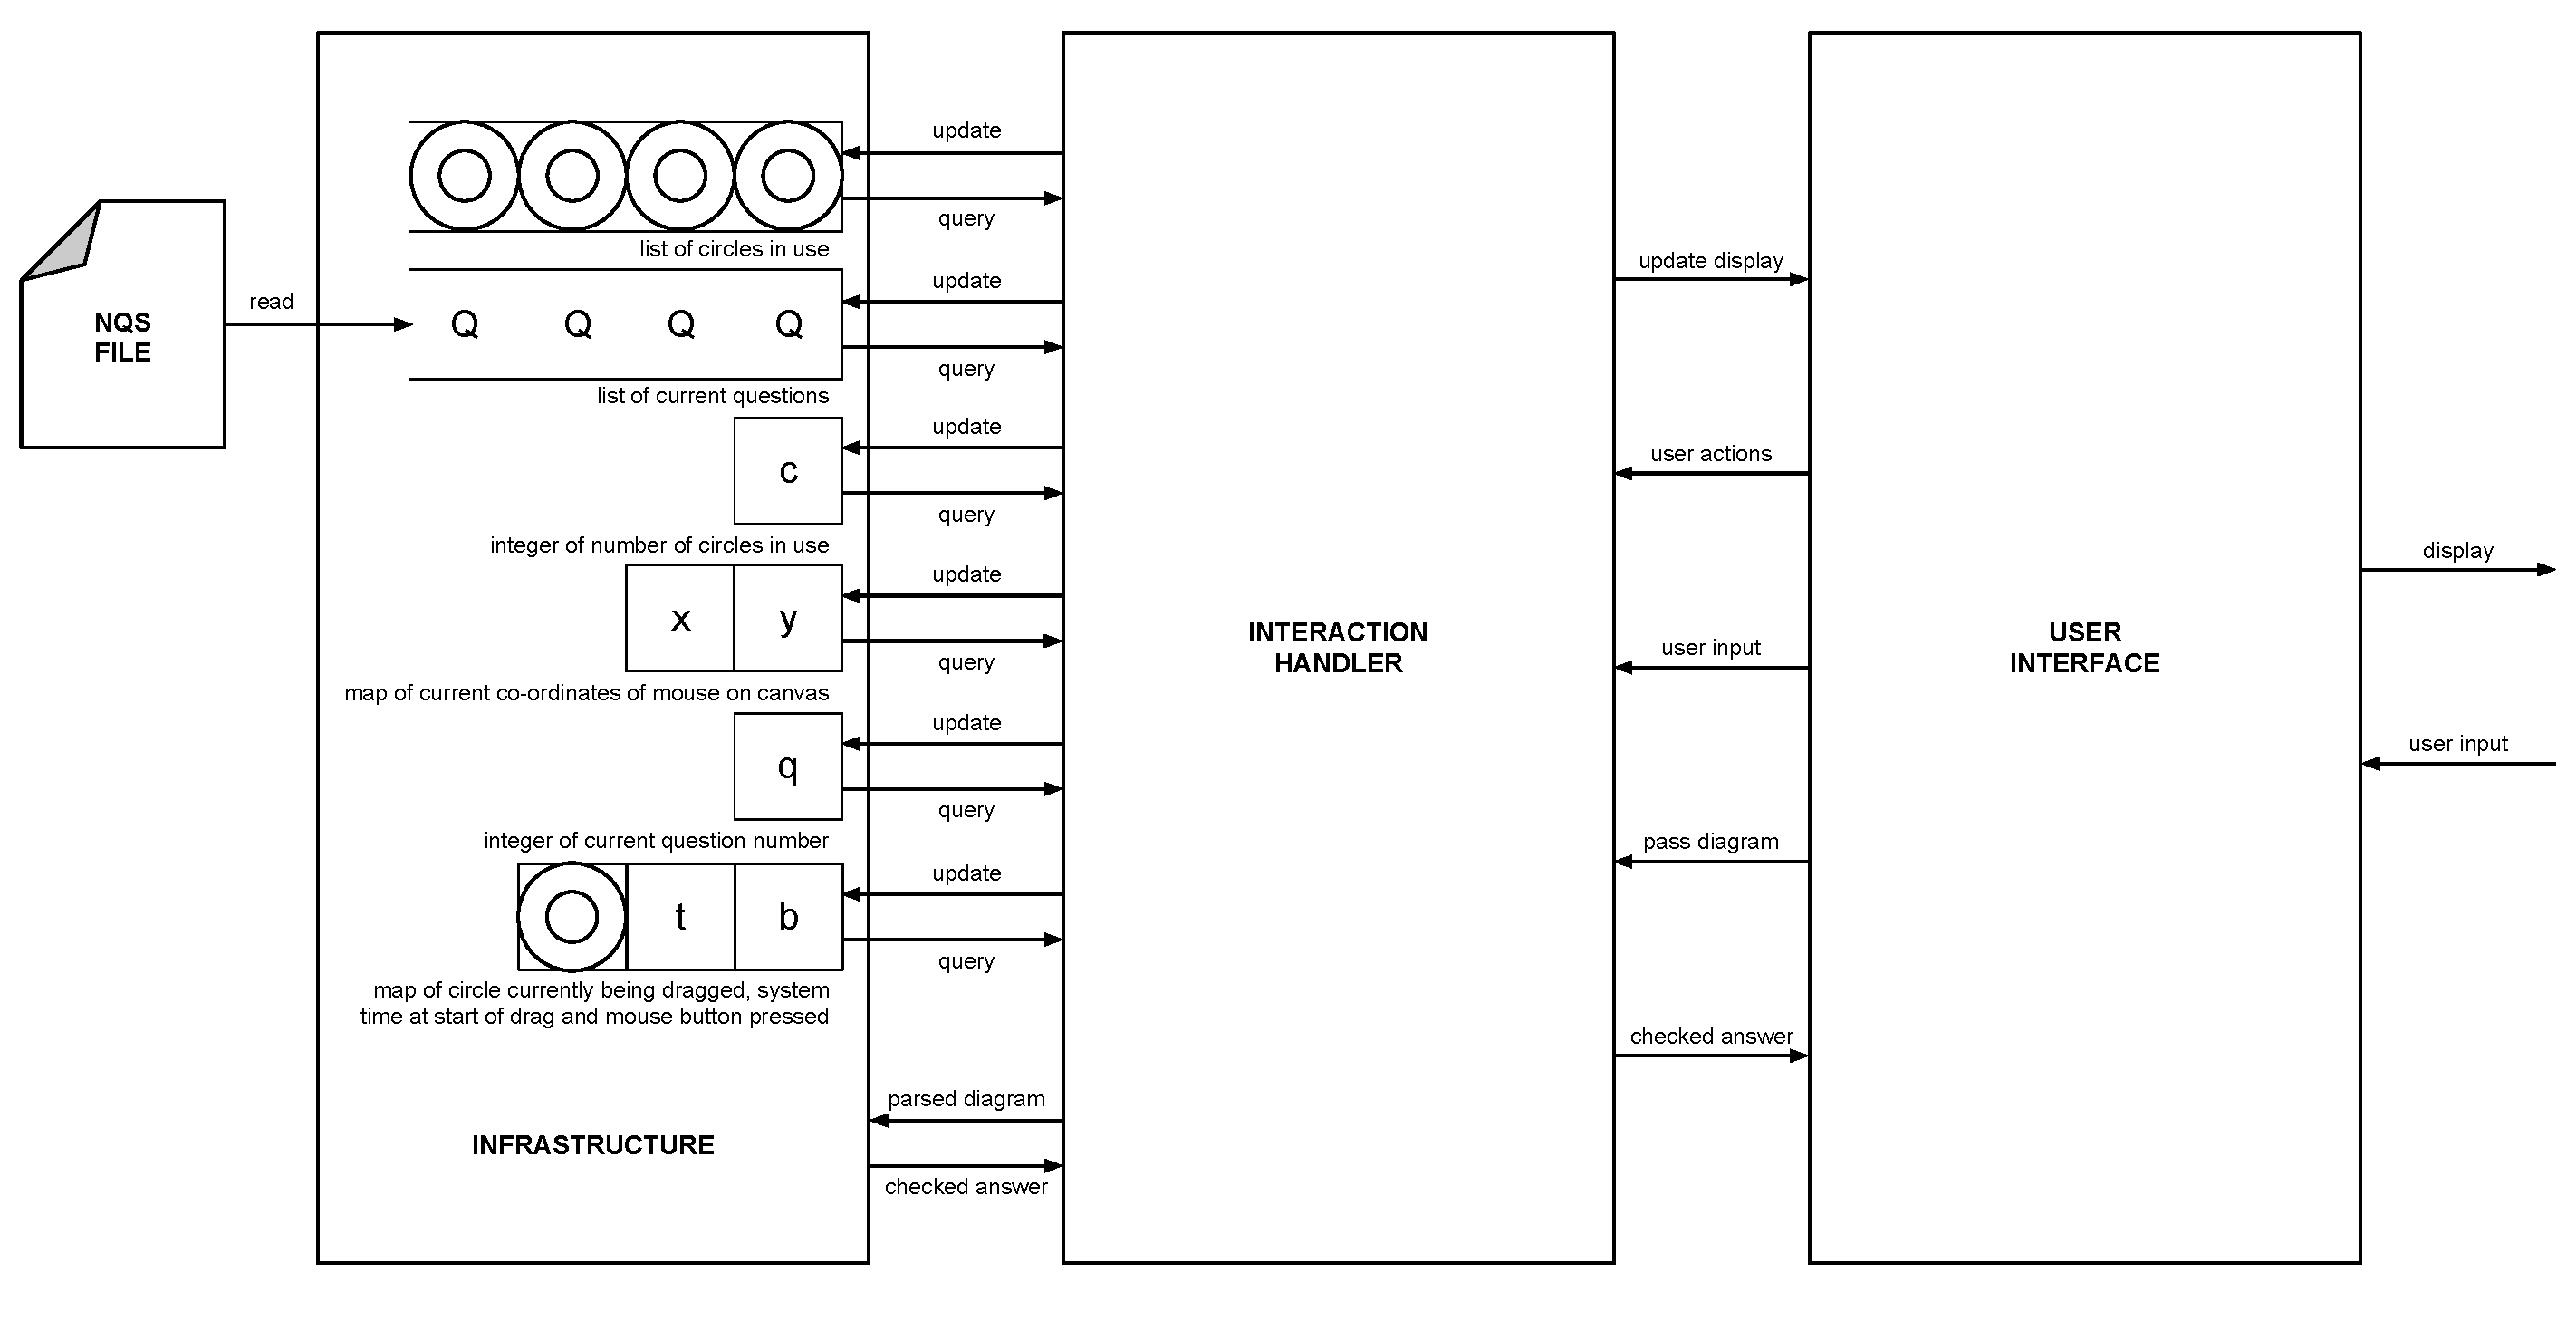
\includegraphics[height=\textheight-2cm]{figs/nico_arch_new.pdf}
\end{center}
\caption{A model of \emph{Nico}'s three-layer architecture.}
\label{fig:NicoArch}
\end{figure}
\end{center}
\end{landscape}

\begin{center}
\begin{figure}[H]
\begin{center}
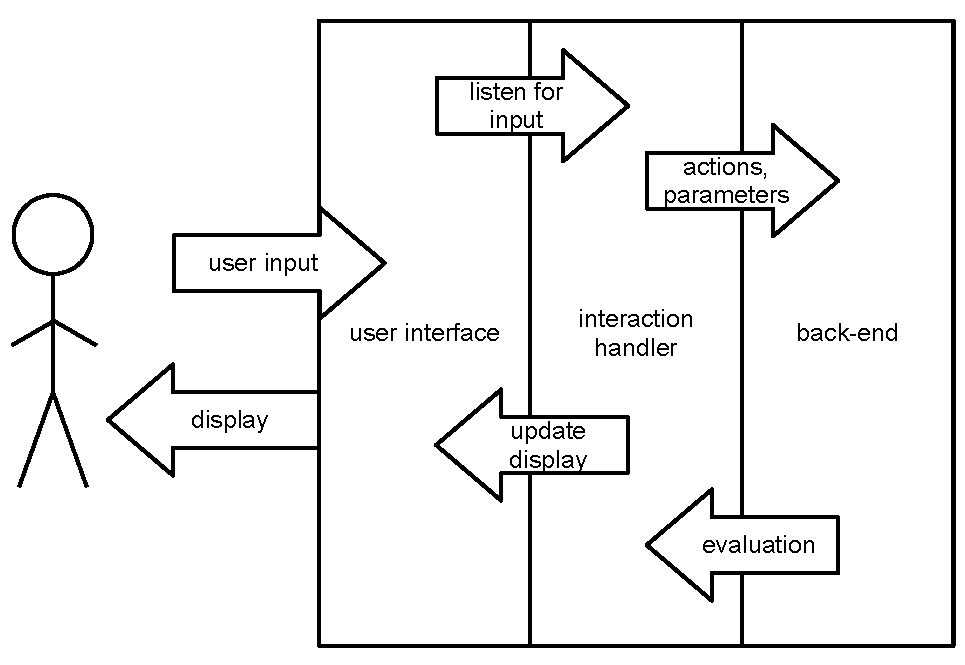
\includegraphics[width=\textwidth-2cm]{figs/nico_arch.pdf}
\end{center}
\caption{A diagram of workflow in \emph{Nico}.}
\label{fig:NicoFlow}
\end{figure}
\end{center}

% TODO: sort out all the pictures, pdfxetex just can't handle that shit (i.e. scaling images - do it in gimp or something)
% TODO: overview of system architecture beforehand
\subsection{Infrastructure}
% calculations as data structures (lists to be evaled)
% rendering engine
% questions and marking
% question syntax
% questions as data structures (lists to be evaled)
% the fact that they are essentially answers means that answers can easily be compared to them, as well as manipulated and stuff - case in point, all the question-highlighting bullshit
% interactivity (300ms rule, see proposal for citation)
% very little mutable state
% placeholders?  why were they introduced?  how did they make things easier?  what problems did they solve?

% TODO: explain components rather than code, make it higher level
The application infrastructure handles mathematical operations; that is, it is able to interpret data from the user's input and process it as a calculation.

Circles could not simply be represented in the application as S-expression versions of the calculations they stood for, as they are not defined solely by their expressions.\footnote{``S-expression'', meaning ``symbolic expression'', refers to nested list data structures that are used in LISP and its derivatives to represent both source code and data.  S-expressions are defined by McCarthy as a single atom, or as an expression of the form {\ttfamily (a . b)}, where {\ttfamily a} and {\ttfamily b} are S-expressions, thus creating a tree structure \cite{McCarthy1960}.}  Data were needed regarding their position on the canvas, so it was decided to use an associative map to represent a circle, containing co-ordinate data as well as the calculation S-expression.

Originally, the program was to use two macros, \verb¬defcircle¬ and \verb¬letcircle¬, to be able to define circles at runtime.  It became apparent that circles defined in this way were not accessible by the interaction handler whilst the program was running.  To solve this problem, `name' data was added to the circle format, and a mutable data structure was chosen to manage a list of circles currently in use.  This allowed the application to access and modify the circles as needed, and also to discard unused circles.

\subsubsection{Management of Mutable State}

\emph{Nico's} infrastructure stores and manages circles and questions using just six mutable data structures:
\begin{itemize}
\item The list of circles, as detailed above
\item The current question set: a list of maps containing the question number and the S-expression that constitutes the question to be answered
\item An integer counting how many circles have previously been created
\item A map containing the current co-ordinates of the mouse cursor
\item An integer indicating the number of the question currently being answered
\item A temporary store for information about circles that are currently being repositioned by the user
\end{itemize}

Mutable data structures were chosen as these elements needed to be continually updated whilst the program was running, and having so few is advantageous.  By reducing the number of elements able to change during the execution of the program, the application is made more stable.  The structure of the application is also easier to test and to comprehend: functions called upon immutable objects will not vary in their output, thus those parts of the program that do not interact with the mutable elements behave predictably.

%\begin{center}
%\begin{figure}[H]
%\begin{center}
%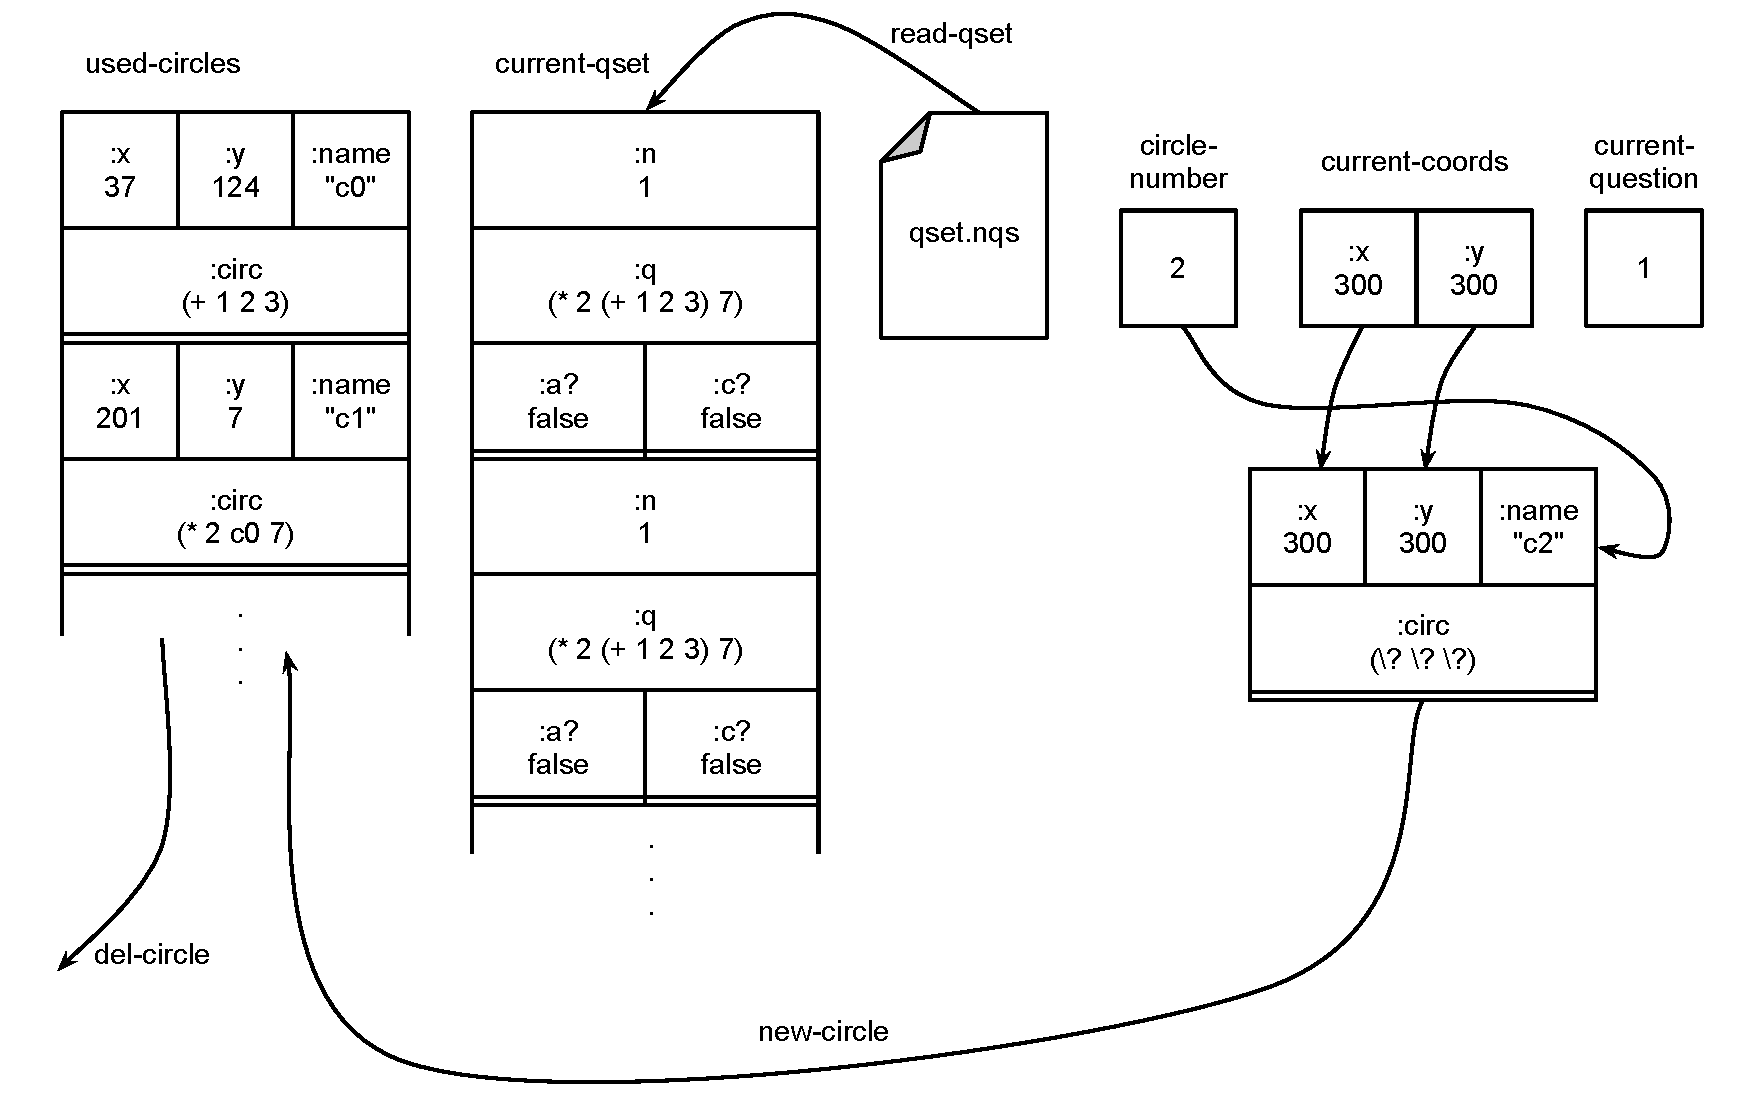
\includegraphics[width=\textwidth-2cm]{figs/nico_backend.pdf}
%\end{center}
%% \caption{A rough model of \emph{Nico's} management of mutable state.}
%\caption{A model of \emph{Nico's} management of mutable state; the sixth agent is omitted as it is not utilised by the back-end.}
%\label{fig:Backend}
%\end{figure}
%\end{center}
%
\subsubsection{Circle Management}

Two main functions for the management of circles have been implemented: creation and deletion.\footnote{Editing of circles is accomplished by deleting a circle and recreating a modified version of it.}  New circles are initialised such that they are centred on the current co-ordinates of the mouse cursor, with a name of the format \verb¬"c¬\emph{n}\verb¬"¬, where \emph{n} is the number of circles previously created.  Upon creating a circle, its expression is initialised to \verb¬(\? \? \?)¬, a meaningless expression using the question mark character \verb¬\?¬ as a placeholder value for both the operator and the two arguments.\footnote{In this dissertation, the placeholder question mark character is represented as {\ttfamily \textbackslash?} when referring to the question mark character literal in Clojure code, and by {\sfapp ?} when referring to the question mark that is displayed for placeholders in the application.}

Placeholder expressions are used so that the user is able to create a circle without having to specify parameters for it beforehand, which would entail \emph{premature commitment}, as well as the \emph{hard mental operation} of having to visualise a circle before committing to creating it.  Such an approach was exhibited with a previous revision of the software, using a complex dialogue box (\emph{Fig.~\ref{fig:GUDB}}).

It was also decided that the circle should use explicitly {\bf placeholder} values, rather than an expression of value 0 (such as (0+0)) so that new circles did not affect the current total displayed by becoming the new root circle (see \emph{Sec.~3.1.1.3} for a full discussion of diagram evaluation).  The placeholders also indicate that action is needed, whereas an expression of value 0 could appear to be a deliberate inclusion in the calculation.

Deletion removes a circle from the list by searching through the main circle list and returning a version which lacks the circle matching either the name or the co-ordinates specified.  The circle list is then updated.

This naïve implementation of deletion led to many problems: it does not deal well with circles that are used as arguments to other circles.  When such a circle is removed from the main list, references to it remain in the circles that were using it, causing the application to throw \verb¬java.lang.NullPointerException¬s.  As such, an alternative version of deletion was implemented, to preserve referential integrity.

The alternative deletion function works by first checking if any of the circles currently in the main list contain references to the circle being deleted.  If it is found that there are circles that do, the function determines if that circle is a root circle (\emph{Sec.~3.1.1.3}).  If so, the root circle is removed using the previous method and replaced, with null references changed to placeholders.  If the circle is non-root, the deletion function recursively calls itself upon the circle, thus removing all circles between the circle to be deleted and the root.  The circle can then be deleted using the original method, and the intermediate circles are replaced.

This solved the problem of maintaining referential integrity, but it has also given rise to a new problem: as the alternative deletion function must call itself upon the other circles in the chain, deleting a circle that forms part of a chain deletes all of the links in the chain between the target and the root.  On reflection, a better way to implement deletion would have been to make the alternative deletion function inspect the main circle list after deletion, checking for any invalid references and replacing them with \verb¬\?¬s, rather than doing so at delete-time.

\subsubsection{Evaluation}

There are two main stages required to evaluate the user's work: finding the root circle, into which all other circles feed, and evaluating a circle or collection of circles to give a valid S-expression.

The root circle is the one circle in a finished diagram that is not used as an argument to any others.  Therefore, it can be found by searching through the list of circles, comparing each one to the rest of the list and discarding it if other circles refer to it.  As stated, in a {\bf finished} diagram, there can only be one root circle, so this method is sufficient for use in marking answers.

It is possible that the user may construct two or more calculation structures in parallel, intending to join them later.  In this case, there can be multiple root circles.  The method chosen to identify the root returns the first instance of a root circle that it encounters.  It would have been possible to, for example, add an extra answer display for each root and to maintain a total for each, but it was decided that this would be confusing, as the user may not expect the structure of the user interface to change.  This would also require reintroducing a labelling system for circles and structures, which was abandoned as it is an unfamiliar concept to non-programmers and those without algebra (the majority of the target audience).

Once the root has been found, the user's diagram can then be evaluated to give an S-expression.  As each circle contains an S-expression for the calculation unit that it represents, the references to other circles can be resolved, creating a nested S-expression that can have Clojure's \verb¬eval¬ called on it to return an answer.

This was, in fact, a significant reason for choosing Clojure; as a homoiconic language, code to be evaluated later can easily be built up as a data structure, which can then be passed around, evaluated and otherwise utilised as is convenient.  By creating one S-expression representing the entire diagram, not only can the value of the structure be calculated, but other operations, such as the selective highlighting of the question display (\emph{Sec.~3.1.2.2}), can be performed.

\subsubsection{Question Management}

Sets of questions are written as external, plain-text files contaning S-expressions corresponding to questions, separated by newlines.  This approach was chosen so that questions can be read into a list using Clojure's standard library, meaning that it is possible to navigate between them by setting the current question to the value of the desired question in the list.

A future extension to this project could be to develop a partner application to \emph{Nico} to aid tutors unfamiliar with LISP to develop their own question sets in a more `user-friendly' manner, rather than by transcribing problems into S-expressions.

\subsection{Interaction Handler}
% the bit that handles all the application shit: render, main-window, etc.
% talk about jfx2 vs. guiftw/swt vs. seesaw/swing
% talk about main-window here i guess?
% talk about dialogue boxes
%
% \emph{{\sc Note:} These paragraphs aren't in the correct order yet; I've just been writing things that I want to include in this subsection, and will reorder them when I have a better idea of where this bit's going.}

The interaction handler forms the `middle layer' of the application (\emph{Fig.~\ref{fig:NicoArch}}) that arbitrates between the infrastructure and the user interface.

The rendering function is called every time the mouse is moved, or when the canvas needs to be updated.  It paints a white rectangle over the canvas area, draws a bin icon in the corner (see \emph{Sec.~3.2.2.2}) and iterates across the circle list, drawing corresponding circles.  References to other circles are visualised as lines extending from the source circle to the appropriate argument slot on the recipient.  By re-rendering every time the mouse is moved, rather than continually, the application does not render when the canvas is not changing.  Every action in the control scheme requires some use of the mouse.

\subsubsection{GUI Libraries}

The original intention of the project was to develop \emph{Nico} using the JavaFX library. However, a number of difficulties were encountered with this: firstly, JavaFX version 2.0 was not available for the primary development environment.  Installation was attempted on a Windows machine, but caused a number of problems. It was decided to proceed using the Eclipse Foundation's SWT toolkit and Szymon Witamborski's corresponding Clojure bindings \cite{GuiFtw}.

During the development of the user interface, many problems were encountered with SWT, particularly regarding drawing arbitrary shapes on the canvas and extracting user input from dialogue boxes.  To keep the project on-schedule, the application was migrated to Java Swing, using the \emph{Seesaw} library to provide bindings for Clojure \cite{Seesaw}.  Development efficiency was increased as a result of the author's previous experience using Swing.

\subsubsection{Main Window}

At the heart of the interaction handler is the structure defining the main window, which comprises the majority of the user interface.  It controls what is displayed and responds to certain conditions.  It listens for certain events (i.e. user input), and prompts the user for input when required.  Seesaw requires interfaces to be structured such that each window is defined as one large structure, with appearance, listeners and other parameters set as options.  Other structures, such as panels and canvases, can then be used as content.

Embedded into the main window are several mouse listeners.  While the application is running, five mouse-based events are listened for: motion, dragging, button presses, button releasees and button clicks.\footnote{It should be noted that a mouse click is defined by Java as a button press followed by a button release, and that, upon a click, it issues a press event, followed by a release event, followed by a click event \cite{JavaApi}.}  When motion is detected, the canvas is cleared and re-rendered.  Motion also triggers a check to determine if the mouse is over a circle; if so, a highlighting function is called, which draws a ring around the circle, and also performs a string comparison.  Using the same function that converts the questions into traditional mathematics for display in the information panel, the circle's S-expression is converted and compared to the question string to see if it appears as a substring.  If so, the appropriate section of the question string is also highlighted, to allow the user to check their work.  It was decided to implement this as a string, rather than S-expression, comparison as the string search is able to return character indices in the question string, indicating the substring to highlight.

\begin{center}
\begin{figure}[H]
\begin{center}
\subfloat[]{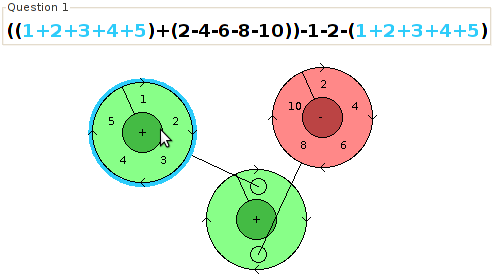
\includegraphics[height=\textwidth/3-1cm]{figs/nico_hi1.png}}
\subfloat[]{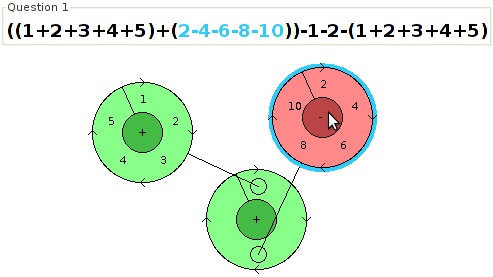
\includegraphics[height=\textwidth/3-1cm]{figs/nico_hi2.png}}
\\
\vspace{0.5cm}
\subfloat[]{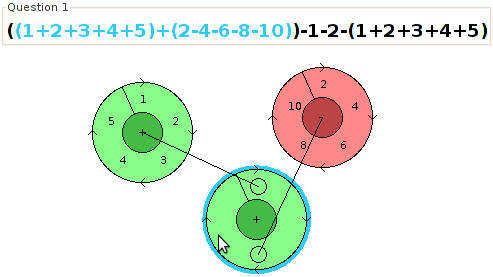
\includegraphics[height=\textwidth/3-1cm]{figs/nico_hi3.png}}
\end{center}
\caption{Three instances of the question text being highlighted as a corresponding circle is moused-over.}
\label{fig:Highlighting}
\end{figure}
\end{center}

\subsubsection{Control Scheme}

Upon detection of a mouse click, the software determines the context in which the mouse was clicked, as this constitutes much of the application's control scheme.  The mouse's current co-ordinates on the canvas, as well as which mouse button was pressed and any modifier keys that were active, are used to determine the correct action to take, as illustrated in \emph{Fig.~\ref{fig:ClickTree}}.

\begin{center}
\begin{figure}[H]
\begin{center}
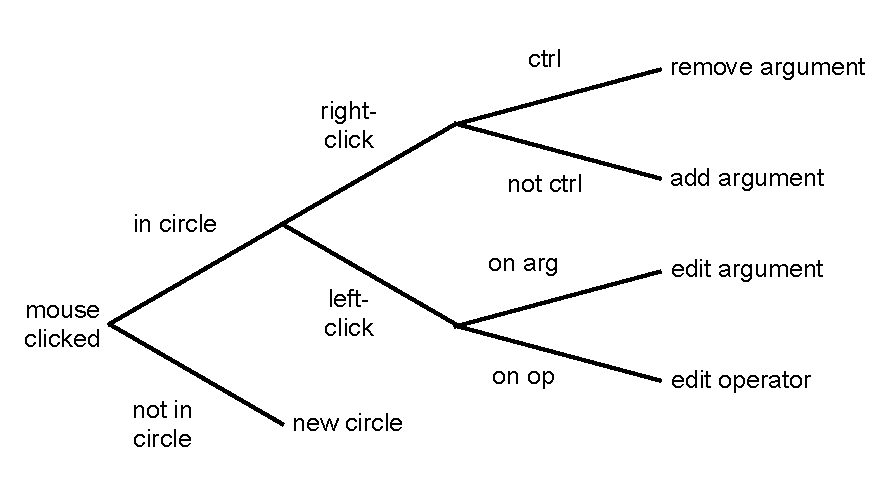
\includegraphics[width=\textwidth-4cm]{figs/nico_click.pdf}
\end{center}
\caption{Decision tree to determine the appropriate response to a mouse click event.}
\label{fig:ClickTree}
\end{figure}
\end{center}

A more in-depth analysis of the control scheme follows.

\begin{itemize}
\item Mouse not in circle
\begin{itemize}
\item A blank circle is created, centred on the current location of the mouse cursor.  It has two arguments, {\sfapp ?} and {\sfapp ?}, and its operator is {\sfapp ?}.
\end{itemize}
\item Mouse in circle
\begin{itemize}
\item Left-click
\begin{itemize}
\item Mouse on argument
\begin{itemize}
\item A small blue circle is drawn around the argument and a dialogue box is launched, using a spinner to set its value.
\end{itemize}
\item Mouse on operator
\begin{itemize}
\item A small blue circle is drawn around the operator and a dialogue box is launched, using four radio buttons to set its value.
\end{itemize}
\end{itemize}
\item Right-click
\begin{itemize}
\item Ctrl key pressed
\begin{itemize}
\item The final argument is removed from the circle.  There is a minimum of two arguments: an alert box warns the user if they try to use fewer.
\end{itemize}
\item Ctrl key not pressed
\begin{itemize}
\item A placeholder argument is added to the circle.  There is a maximum of eight arguments: an alert box warns the user if they try to use more.
\end{itemize}
\end{itemize}
\end{itemize}
\end{itemize}

Drag-and-drop functionality is also included in the control scheme.  When the application detects that a mouse press has occurred, if the event was triggered whilst the mouse cursor was over a circle, that circle is stored with the current system time and the button that was pressed in a mutable data structure.  When a drag event is detected, that information is then used to perform one of two operations upon the circle.

If the left mouse button is held whilst dragging, the circle's co-ordinates are updated to the current co-ordinates of the cursor.  If the right mouse button is held whilst dragging, a line is drawn from the circle to the current location of the cursor.  When the mouse passes over the argument slot of another circle, that line is fixed, and the target circle is updated such that the argument is now a reference to the source circle.

The drag-and-drop functionality was implemented thus as a drag-and-drop action constitutes a press event, followed by a drag event, followed by a release event.  By storing information about the circle being dragged when the mouse is pressed, the function called upon dragging can use and modify this information easily.  This does not impact upon other mouse events involving presses and releases (e.g. clicking), as this information is discarded upon every mouse release, regardless of whether or not it was being used.

The control scheme is almost entirely mouse-based as the mouse is a simpler interface than the keyboard, and is familiar to most computer users in a school environment, regardless of ability (the use of applications that require mouse control, such as many word processors, is mandated by the National Curriculum).  By limiting control to the mouse, the user is required to remember fewer button locations, and is likely to be able to guess controls correctly if forgotten.  A caveat to this is that the use of the Ctrl key is required, as this was preferable to mouse chording (unfamiliar to novices), or to requiring a three-button mouse (not always available).

The design of the control scheme is discussed further in \emph{Sec.~3.2.2}. % TODO: check this, gonna rearrange massively

% do i need to mention *all* the times clear-screen and render are called?  it's kind of implicit (to me anyway)...
%
% \emph{{\sc Note:} This is as far as I've got (about halfway by my reckoning).  }\verb¬texcount¬\emph{ tells me I've got about 5,800 words.}
% \subsection{User Interface}
% do we even need this section?  applciation below might cover it, and to be fair it isn't really part of the architecture - listeners and that should probs go in interaction handler above
%
\section{User Interface}%{Application}
% application in which the language is manipulated
% talk about how the app has changed, show screenshots
% talk about how the app becamse more minimalist, to focus on the language itself
% language as a main focus, with useful information n shit around it in the app
% colour-coding text (though consider colour-blindness with the red and green text)
% question highlighting - talk about troubles with it, but also merits of including it
% do we need this section?  shouldn't this be the ui bit in the prev. section?
% have lost the ui bit in favour of having this as a separate section
% target audience - children (year 5), but also applications in remedial adult learning (i.e. can't be too childish)
% hence must be appealing, clear, easy-to-read, not too verbose
% prototypes! take screenshots of old versions

The user interface comprises the parts of the application which are user-facing; that is, they are that which the user directly interacts with.  The development of \emph{Nico}'s user interface was key to the success of the overall project, being primarily an experiment in human-computer interaction.

During its development, \emph{Nico}'s user interface went through a number of revisions.  Details of how the UI design developed over time follow.

\subsection{Application}

\begin{center}
\begin{figure}[H]
\begin{center}
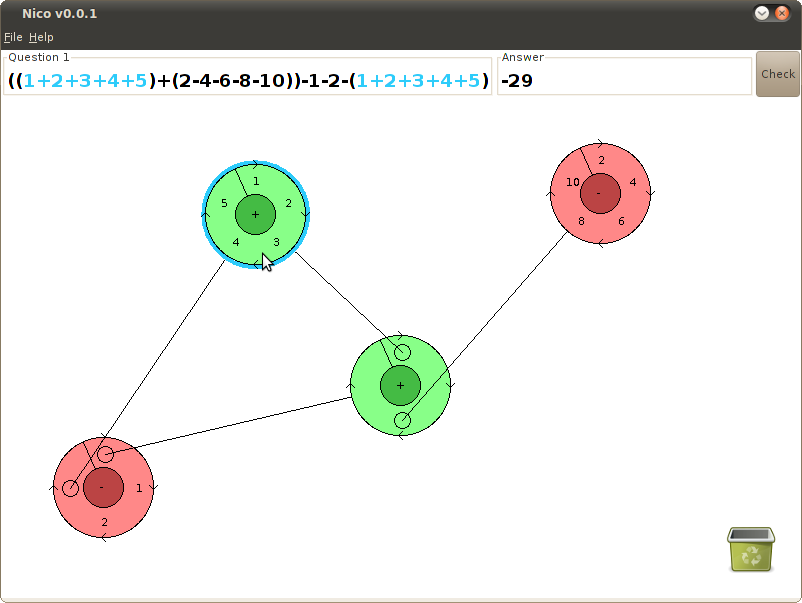
\includegraphics[width=\textwidth]{figs/nico_screen_01.png}
\end{center}
\caption{A screenshot of a \emph{Nico} session.}
\label{fig:Nico1}
\end{figure}
\end{center}

The application itself was kept fairly minimal: the aim was to emphasise the notation as the most important aspect of the software.  As such, the main application window, as shown in \emph{Fig.~\ref{fig:Nico1}}, is mostly dedicated to the canvas area in which the user answers the question.

The main application window is split up into two main sections, the information panels that display the question being answered and the current total of the user's calculation, as well as the {\sfapp Check} button to submit the current total as the answer, and the large canvas area in which the user is able to construct diagrams with which to answer the question.

\subsubsection{Initial Revision and Control Buttons}

Initially, the application was intended to use more buttons (see the prototype in \emph{Fig.~\ref{fig:ProtoCirc}}, above), having more controls immediately visible to the user.

In the first usable version of the interface, there were a number of buttons that appeared down the side of the application.  These had been relocated to save screen estate, keeping the canvas free for the sole use of the notation.  Each button ({\sfapp New}, {\sfapp Edit}, {\sfapp Delete}, etc.) would cause a dialogue box to appear to the user, which required a circle to be specified by name (at this point in the development of the project, it was required that the user name each of their circles) before any operations could be performed upon it.

This design was abandoned as the separation between the user and the diagram itself was too great; creating circles by specifying options in many only slightly different dialogue boxes and watching the results appear on the canvas did not feel like a natural way to interact with one's calculation, and hence would have been inappropriate for the target audience.  Indeed, forcing the user to commit to a design before even seeing it entailed much \emph{premature commitment}, and having to re-express circles to edit them greatly increased \emph{viscosity}.

\subsubsection{Context Menus and Automated Marking}

Later revisions of the software removed the buttons and implemented a system of context menus with which to construct answers, to further increase the space available for the user's answer, and to make the link between performing an action and its consequence more evident (e.g. right-clicking on a circle and seleting `Delete', rather than choosing to delete a circle and specifying the target's name); this way, the user was able to interact with the canvas itself, rather than pressing buttons at the side.  The many dialogue boxes were combined into one (\emph{Fig.~\ref{fig:GUDB}}), used for both the creation and modification of circles.

Answer-checking was also made automatic: as soon as the total reached a value equal to that of the answer to the question, the user was immediately told so, and moved on to the next question.  The intention here was to streamline the user's experience, increasing their efficiency (i.e. the speed with which question sets were completed).

This design was ultimately abandoned as, again, it separated the user from their own work too much.  Although this design was an improvement, allowing the user to interact directly with the canvas to perform operations upon circles that were able to specified by pointing with the mouse, rather than by specifying an action and typing out a name, the dialogue box was too complex, and still entailed the \emph{premature commitment} of the user by requring a circle's specification before creating one.

The automatic answer-checking was also a problem, as it did not give the user a chance to review their answer before proceeding.  Indeed, it did not give the user a chance to learn from their mistakes; for example, if they had accidentally reached the right answer as part of a larger, incorrect calculation that they had previously intended to make.

\subsubsection{Final Revision}

The final revision of the software reintroduced the {\sfapp Check} button to address the issues with the automatic answer-checking in the previous version of the application, and replaced the system of context menus with a new control scheme, as discussed in \emph{Sec. 3.2.3}.

\begin{center}
\begin{figure}[H]
\begin{center}
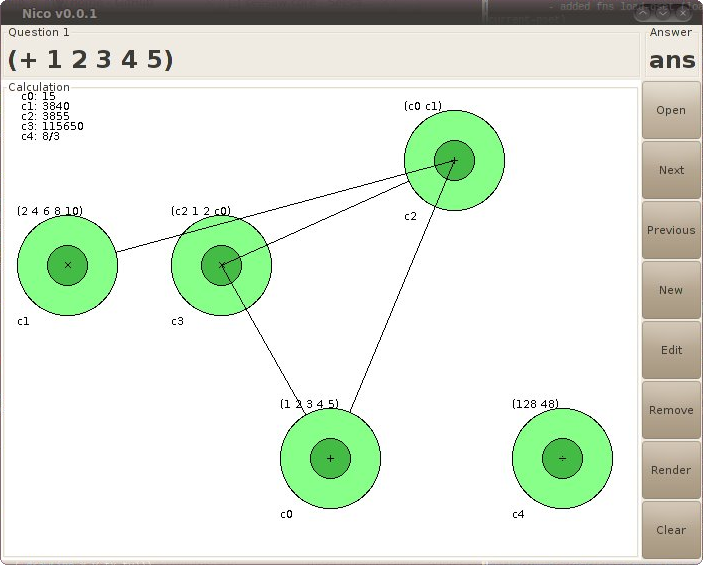
\includegraphics[width=\textwidth-4cm]{figs/nico_screen_oldest.png}
\end{center}
\caption{A very early version of the user interface.  Many features are yet to be implemented, but the layout with the buttons and the early revision of the notation is evident.}
\label{fig:OldApps1}
\end{figure}
\end{center}

\begin{center}
\begin{figure}[H]
\begin{center}
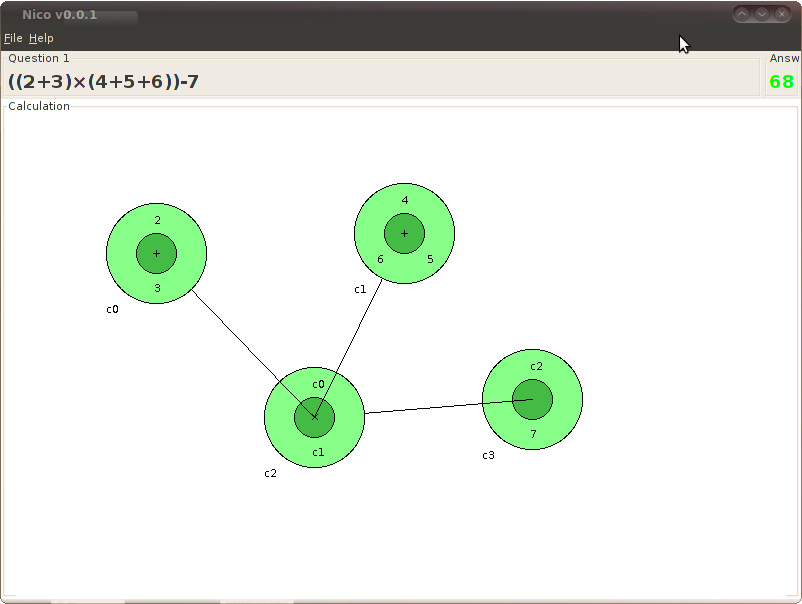
\includegraphics[width=\textwidth-4cm]{figs/nico_screen_older.png}
\end{center}
\caption{A later revision of the user interface.  The screen has been cleared, allowing context menus to replace buttons.  The facility for checking an answer has been removed, due to the automatic answer-checking in this version.  The notation has now been fully implemented, but still lacks many features of the final version.}
\label{fig:OldApps2}
\end{figure}
\end{center}

\begin{center}
\begin{figure}[H]
\begin{center}
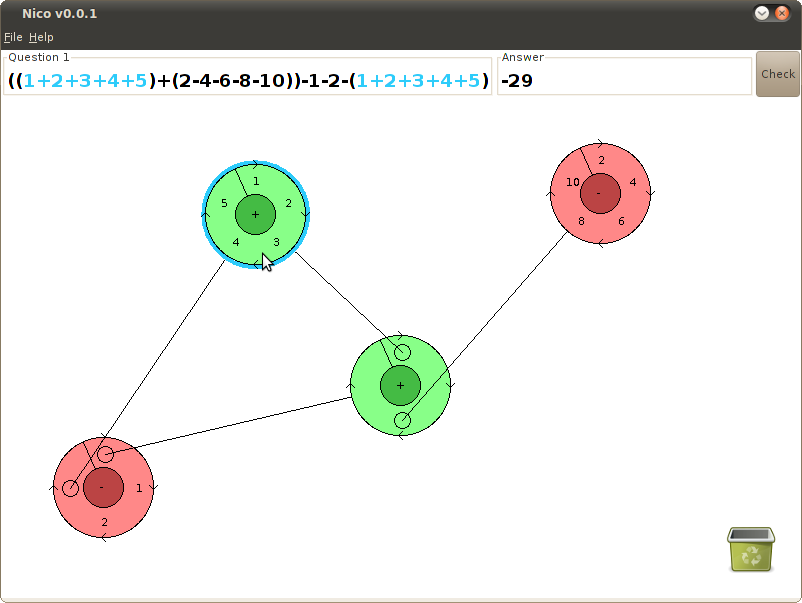
\includegraphics[width=\textwidth-4cm]{figs/nico_screen_new.png}
\end{center}
\caption{The final revision of the user interface.  The layout is similar to the previous version, but now includes highlighting and the bin icon for deletion.  The notation is now colour-coded, and the answer-checking button has been reintroduced.}
\label{fig:OldApps3}
\end{figure}
\end{center}

\subsubsection{Dialogue Boxes}

Dialogue boxes have been a consistent feature of the user interface since its first revision.  Initially, dialogue boxes were triggered by the buttons at the side of the application (\emph{Fig.~\ref{fig:OldApps1}}), and consisted of a simple text field, into which the user typed a circle's name, followed by, in the case of the creation and editing of circles, an S-expression specifying the mathematical expression that the circle was to represent.

This was never intended to be the final version of the user interface, but was useful for testing the rest of the user interface and interaction handler at the time.  Requiring a user to be familiar with LISP syntax ran somewhat counter to the intentions of this project, being to provide an accessible alternative notation for arithmetic for the non-programmer, pre-algebra user.

\begin{center}
\begin{figure}[H]
\begin{center}
% \includegraphics{figs/nico_gudb.png}
\includegraphics[height=\textheight/2-2cm]{figs/nico_gudb.png}
\end{center}
\caption{The unified dialogue box.}
\label{fig:GUDB}
\end{figure}
\end{center}

In later revisions of the software, as mentioned in the previous section, the many dialogue boxes were combined into one, with many options available to specify the parameters of a circle.  This was implemented to eliminate the need for typing in S-expressions, as in the previous incarnation of the user interface, and dynamically generated its layout, making new circles available to use as arguments as they were created.

It was decided to combine all parameters into one dialogue box (\emph{Fig.~\ref{fig:GUDB}}), rather than many smaller dialogue boxes, with the intention of streamlining the user experience by providing all available controls in one location.  However, the grand unified dialogue box still required the user to perform operations without it being entirely obvious what the consequences would be, thus requiring an unnecessary amount of \emph{premature commitment} from the user.  In addition to this, the act of visualising the circle to be created whilst setting the many options available in the dialogue box constituted a superfluous \emph{hard mental operation}, and actually required {\bf more} time to search for information than several simpler dialogue boxes, in which less information is presented at once.

In the final revision of the software, the dialogue boxes were reduced down to two small instances, as shown in \emph{Fig.~\ref{fig:Dialogues}}, used in combination with the new control scheme.  It was acknowledged that the large dialogue box was unwieldy and dense, requiring the user to search for controls within it and increasing the \emph{viscosity} of the notation by requiring all parameters to be set every time one needed to be edited.

The two simple dialogue boxes served to greatly decrease this \emph{viscosity}, making it so that single arguments or operators could be edited independently of the rest of their circles.  In combination with the improved control scheme, this helped to eliminate much of the \emph{premature commitment} of previous designs, by making the creation of a circle an incremental process, rather than a single event.

\begin{center}
\begin{figure}[H]
\begin{center}
\subfloat[Editing a circle's operator]{
\includegraphics[width=\textwidth/2-2cm]{figs/nico_op.png}
}
\subfloat[Editing a circle's argument]{
\includegraphics[width=\textwidth/2-2cm]{figs/nico_arg.png}
}
\end{center}
\caption{The dialogue boxes used to modify existing circles in the application.}
\label{fig:Dialogues}
\end{figure}
\end{center}

\subsection{Control Scheme}

% TODO: diagram?  like the one in the notebook, showing the consequences of each possible action to illustrate the control scheme and notation
% why the '(\? \? \?) initial circle expr?

\subsubsection{Development}

Initially, the application used a collection of buttons and dialogue boxes, as detailed above, to control the circles that appeared on the canvas.  This was implemented to ensure that the user interface was functional, and so that circle operations could be tested.  It was abandoned as it required too much \emph{premature commitment} from the user, who would have to consider the consequences of performing an action before doing so.

In later revisions, a system of context menus was implemented to decrease the separation between the user and their work.  Right-clicking on a blank patch of the canvas gave the user the option to create a new circle, and right-clicking on an existing circle presented the user with the option to either edit or delete that circle.  This required less forethought on the part of the user, but the use of the unified dialogue box (\emph{Fig.~\ref{fig:GUDB}}) still entailed some \emph{premature commitment}.

The control system is now predominantly mouse-based for the construction of calculations in the application's notation, as detailed in \emph{Sec.~3.2.1.3}.

\subsubsection{Control Design}

Left-clicking on a blank patch of canvas creates a new circle, initialised with two arguments, {\sfapp ?} and {\sfapp ?}, and with operator {\sfapp ?}.  This approach was chosen, rather than providing the user with a null circle such as (0+0), to make it clear to the user that the new circle required attention, and so that it wouldn't interfere with the evaluation of the diagram; a new circle on its own could be found to be a root circle, leading to the possibility that the user's total could suddenly drop to 0.

Right-clicking on a circle increments its number of arguments by one, up to a maximum of eight.  Holding the Ctrl key and right-clicking on a circle decrements its number of arguments by one, down to a minimum of two.  The user is warned by a popup if the exceed either of these boundaries.  The limit of two to eight arguments was decided upon as fewer than two arguments is an unfamiliar and not often useful concept from the perspective of the target audience.  Although Clojure is able to evaluate, for example, \verb¬(+ 1)¬ (returning \verb¬1¬), this is liable to lead to confusion on the part of the user.  The upper limit of eight arguments was set to prevent circles from becoming overcrowded and thus harder to read.

Circles can be moved around the canvas by left-clicking and dragging the circle to the desired location.  If a circle is dragged to the bin icon in the bottom left-hand corner of the screen, then it is removed.  Originally, deletion was mapped to a mouse control, but in the interest of a simpler control scheme and with a limited number of mouse buttons, it was decided that an icon should be used instead.  This also has the advantage of demonstrating to the new user that work can be easily undone, encouraging exploration.

Left-clicking on a circle's operator brings up a dialogue box with a selection of operators in it, with a radio button for each (see \emph{Fig.~\ref{fig:Dialogues}}).  Similarly, left-clicking on a circle's argument brings up a dialogue box containing a spinner, which can be used to set a new value for that argument, between -10 and 10.

The spinner is limited to this particular range as this prevents the user from using the software as a calculator.  The limited range of numbers available means that the user must still consider strategies such as partitioning or long multiplication, focussing on how to solve the problem, rather than simply transcribing the question into one circle that will complete the calculation for them.  The user is not required to calculate manually expressions using such small numbers, as it is assumed that the target audience are familiar with simple arithmetic.

To use one circle as an argument to another, right-clicking and dragging allows the user to drag a line ending in a circle to the desired slot on the recipient circle.  By having the user pull links out from existing circles, as opposed specifying references and links consequently appearing, the direction of dataflow is emphasised.

This new control scheme allows the user to feel more like they are directly manipulating their work in progress, with each action having clear consequences.  It reduces the \emph{viscosity} of editing circles from the previous controls schemes of butons and context menus, and greatly reduces the amount of \emph{premature commitment} required of the user when creating circles.  It creates an environment that encourages exploration, and does not require the user to spend time searching for information within parts of the user interface.

\subsection{Colour-Coding}

% talk about colour-blindness
% why this colour scheme? psychological reasons?
% why not random or connection-based colours?
\emph{Nico} uses colour-coding in various areas of the application, to draw attention to important elements of the application.  Colour-coding has been shown to faciliate more effective learning.  Indeed, Lamberski and Dwyer note that
\begin{center}
\parbox[c]{\textwidth-2cm}{
\small
``[...] younger learners, for whom color in passive materials has been found to facilitate performance in less complex concept attainment tasks because of color's attention of motivation elements.  However, when younger learners have been given self-paced instructional materials containing color-coded reading and phonic concepts, similar positive results have been attained.'' \cite{Lamberski1983}
}
\end{center}
\emph{Nico}'s colour scheme was implemented incrementally over the course of the project.  It was originally intended, as shown in \emph{Fig.~\ref{fig:ProtoCirc}}, to be based on how nested a circle was.  This was rejected on the grounds that it could become confusing if a circle were reused (see \emph{Fig.~\ref{fig:Nico2}}).  Consequently, circles are coloured according to their operators, clearly separating different kinds of operations and making the notation more \emph{visible}.

\begin{center}
\begin{figure}[H]
\begin{center}
\includegraphics[width=\textwidth-2cm]{figs/nico_screen_02.png}
\end{center}
\caption{An example of where nesting-based colour-coding would be confusing.  The circle containing (2+2) can be considered to be both one and two circles removed from the root circle.}
\label{fig:Nico2}
\end{figure}
\end{center}

Colour-coding is also used in the information panels: positioning the mouse cursor over a circle highlights the part of the question that it is likely to represent in blue, and also highlights the circle with a blue outline.

When an answer is submitted, the text in the answer panel turns red if the answer was incorrect, or green if the answer was correct, providing an unintrusive form of feedback, allowing the user to continue uninterrupted (i.e. no input is required to continue) if their answer is wrong.

\begin{center}
\begin{figure}[H]
\begin{center}
\subfloat[Red text indicates that the answer submitted was incorrect]{
\includegraphics[width=\textwidth/3]{figs/nico_wrong.png}
}\hspace{2cm}
\subfloat[Green text indicates a correct answer; a dialogue box allows the user to progress to the next question when they are ready]{
\includegraphics[width=\textwidth/3]{figs/nico_right.png}
}\\
\subfloat[The circle's operator is highlighted when it is being edited]{
\includegraphics[width=\textwidth/3]{figs/nico_op_hi.png}
}\hspace{2cm}
\subfloat[An argument is highlighted when it is being edited]{
\includegraphics[width=\textwidth/3]{figs/nico_arg_hi.png}
}
\end{center}
\caption{Examples of colour-coding in \emph{Nico}.}
\label{fig:ColourCoding}
\end{figure}
\end{center}

\subsubsection{Colour Blindness}

As \emph{Nico}'s notation and user interface are quite reliant upon colour to express or emphasise information, colour-blind users are liable to find some parts of the application confusing.  As such, although no functionality to address this was included in the application itself, the colours used thoughout are easily replaced in the source code, being defined early on and with the variables, rather than simply numbers, referred to throughout.  By changing the variables for each circle's colours, it is possible to create customised versions of the software to suit individual cases of colour blindness.  For example, a person with total colour blindness may need a version of the software that uses shades of grey, rather than colours, people with other forms of colour blindness, such as protanopia or tritanomaly may only need to replace certain colours in the application's colour scheme.% TODO: implement this!

\subsection{Notation}%metaphor?

% graphical language itself
% show previous versions
% talk about how the circles have to make clear e.g. arg order
% talk about how circles had to be improved, show iterations
% more screens: old versions of the language to compare
\begin{center}
\begin{figure}[H]
\begin{center}
\subfloat[An old version of the notation.  Circles are uniformly coloured, and links feed into the centre of their target circles.  There is no indication of argument evaluation order.]{
\includegraphics[width=\textwidth/2-2cm]{figs/nico_notn_old.png}
}\hspace{1cm}
\subfloat[The final version of the notation.  Circles are colour-coded by operation, highlighting has been implemented and links fill argument slots, ending in a circle to indicate their destination.  The diagonal line and arrows have been added to circles to indicate evaluation order.]{
\includegraphics[width=\textwidth/2-2cm]{figs/nico_notn_new.png}
}
\end{center}
\caption{The notation used also went through a number of revisions before reaching its current state.}
\label{fig:OldNots}
\end{figure}
\end{center}

The notation itself was also revised several times during the development of the application.  The original vision of the notation can be seen in \emph{Fig.~\ref{fig:ProtoCirc}}.  It was decided to move slightly away from this model, as much of the circles' decoration occupied an unnecessary amount of screen estate. As such, it was decided to replace the curved link design with simple lines, allowing many linked circles to be closer together but still \emph{visible}.

The first implementation of the notation consisted of uniformly-coloured circles connected by lines feeding into the centre of the recipient circle.  The lines fed into the centre of the circle so that links to circles would not restrict further the number of available arguments per circle.  The colour scheme had simply not yet been implemented.

There were no placeholder values; these were unnecessary as the system of dialogue boxes meant that at no point could a circle have any
aspect of itself in an undefined state.  There was also no indication of argument ordering, which is acceptable when the operator is commutative (i.e. addition or multiplication), but for operations where this is not the case, this can quickly become confusing.

Although the ordering and placement of arguments was defined, with no indication of this, the user is required to figure this out through experience, which is counter to the intentions of the software.  It should not be required that the user spend a significant amount of time learning how to use the system, especially due to deficiencies in the notation.

Another, greater, problem related to argument ordering was that of the circles that linked to other circles.  With all input circles pointing to the operator at the centre of their target circle, it was not at all clear in which order the input circles evaluated, neither relative to each other nor to the other arguments in the circle, which would have been problematic in situations where one circle was used as an argument to several others.

% TODO: poss. a figure showing close-ups/details of newest notation?
The design of the notation was changed to address the problems listed above.  In its final revision, the notation has had a number of features added.

Firstly, the circles are now colour-coded by operator, making it easier for the user to distinguish between different kinds of circles.  The circles themselves have also been embellished slightly with the addition of a line denoting the start of the expression, just to the side of the first argument at the top of the circle.  Small arrows have also been added to the edge of the circles to indicate in which direction the arguments should be read.  Finally, the links between circles have been changed such that they now occupy an argument slot that could otherwise be taken by a number, with a circle on the end of the link line to clearly show where the link terminates.
% TODO: more cogdims!  ALWAYS more cogdims!
% TODO: testing?  or does that go in the next chapter?

\section{Testing}

Development of the software was primarily REPL-driven, allowing for rapid development and testing whilst the application was running.  A suite of tests were derived from assertions made in the REPL.  The fact that the system had few mutable elements meant that most of it behaved very predictably; the only components which required integration testing were those that interacted with the application's mutable structures, thus reducing complexity.% TODO: this bit, wtf
%
%5Throughout the development of the software, unit tests were performed to ensure the integrity of the code.  GNU Emacs, in combination with SLIME/SWANK and clojure-mode, includes functionality such that commented-out lines of code can be evaluated at will.  As such, it was possible to write unit and integration tests into the main body of my code and to evaluate them whenever a change may have affected how a function behaved.  In the interests of tidiness and code readability, many tests were removed as they became unnecessary later on in the development in the project.
%
%% TODO: chat shit about assertions
%Assertions were also used to perform tests: Clojure provides the developer with the ability to specify runtime tests as part of function definition, throwing exceptions if any assertions.  Such tests were used in addition to the previous method to unit-test and integration-test the functions within the application.

\section{Summary}

In this chapter, the implementation of the project was discussed in some detail, as well as the challenges that were faced during this development phase.

The software itself fulfils and exceeds the criteria for success outlined in the project proposal, being a complete and usable system that improves greatly, in terms of cognitive dimensions, upon the traditional method of handwritten arithmetic.

Third-party libraries, in particular Seesaw, were used where appropriate.

The application divides into three main sections: the infrastructure, handling mathematical operations and memory management, the interaction handler, helping the user interface to interface with the infrastructure, and the user interface itself.

Mutable state was introduced where necessary, but kept to a minimum.  The application uses just six mutable data structures, meaning that functions not interacting with these object will behave predictably, making the software easier to comprehend and test.

The user interface was revised many times to correct deficiencies in the design that would have led to a poor user experience, and the infrastructure and interaction handler were also both restructured as new demands upon the software became apparent.

In the next chapter, the software will be evaluated, discussing test results and the user study that was conducted as an extension to the project.

\cleardoublepage
\chapter{Evaluation}

This chapter concerns the testing and evaluation of \emph{Nico}; carried out to determine the quality and utility of the software.

\section{Testing}% {Defect Management and Testing}% {Backend Testing}
% used slime/swank with test lines as comments to be evaluated with C-x C-e
% emacs/slime/swank as ide; ideal for lisps!
% lein test framework - need to actually set up some tests first though!
% clojure test-is; see http://en.wikibooks.org/wiki/Clojure_Programming/Tutorials_and_Tips#Unit_Testing_in_Clojure

% does C-x C-e *actually* count as unit testing?  i mean, i *did* test small bits and then test bigger bits after i'd established that the smaller bits worked...
% apparently it does! w00t
% also talk about integration testing (after the units have been tested, testing the bits that use those units), and see the link in alistair's email re other levels of testing
%Throughout the development of the software, I performed unit tests to ensure
%the integrity of my code.  My development environment of choice, GNU Emacs
%using SLIME/SWANK and clojure-mode, includes functionality such that
%commented-out lines of code can be evaluated at will.  As such, it was possible
%for me to write unit and integration tests into the main body of my code, evaluating them
%whenever a change may have affected how a function behaved.  In the interests
%of tidiness and code readability, many tests were removed as they became
%unnecessary later in the development in the project, but \emph{Fig.~\ref{fig:SlimeTests}}
%shows one of the test blocks that were left in the most recent revision of the
%source code.

\section{UI Evaluation}
% user testing
% graphs
% 300ms test - see below (under goals)
% maybe time render too?

The time taken to generate an S-expression, evaluate it and display the result to the user was required by the project proposal to be less than 300ms.  To test this, a \emph{Nico} session was completed, using the same questions as in the user study (below), but with a modified version of the function \verb¬update-answer¬, which generates an S-expression from the user's diagram, evaluates it and displays the result to the user, that included functionality such that the system time upon entering and exiting the function was recorded in an external log file.

A plot of the time taken for each call to \verb¬update-answer¬ to complete over time is shown below.

\begin{center}
\begin{figure}[H]
\begin{center}
\subfloat[]{
\includegraphics[width=\textwidth-2cm]{figs/graphs/update_times_full.png}
}\\
\subfloat[]{
\includegraphics[width=\textwidth-2cm]{figs/graphs/update_times_cut30.png}
}
\end{center}
\caption{a) Plot and b) detail of the time taken for {\ttfamily update-answer} to complete, over the course of one session.}
\label{fig:UpdateTimes}
\end{figure}
\end{center}

\emph{Nico}, in almost all cases in which a measurement was taken, was able to interpret the user's diagram and display the result in much less than the upper limit of 300ms, with a mean time of 6.751852ms.  Of the 810 samples taken, there was one anomalous time of 308ms.

% \subsection{Notation Evaluation}
% % user testing
% % graphs
%
\section{User Study}
% results
% pilot study - ellie suggested switching left/right-clicks in control scheme, implemented before main study

To assess the utility of the software relative to handwritten arithmetic, a user study was conducted, allowing real users to get to grips with the system, and provide feedback on it.  To this end, users were given a tutorial video and a questionnaire (see \emph{Appendix C} for the full questionnaire) to complete whilst using the software.

\subsection{Experimental Design}

Originally, it was the intention of this project to perform a user study upon a `test class' of Year 5 pupils at an actual school, but the ethical complications involved with working with vulnerable individuals were so great as to make such a study impractical, given the time constraints of this dissertation; in addition to obtaining the approval of the Ethics Committee and the permission of a school to conduct the study, consent forms would have to be distributed to the test class, taken home, signed by the pupils' guardians, returned to the school and returned to the author.  It was, therefore, decided that the software should be tested upon a group of students not currently reading a `mathematical' subject, such as the Natural Sciences Tripos, the Mathematical Tripos or the Computer Science Tripos, which necessitate a high level of mathematical aptitude and experience.

Participants were first asked to sign a statement of informed consent, giving their consent to participate in the study, and were then asked if they had previously used \emph{Nico}, and to indicate their confidence in their ability to solve simple mathematical problems on a five-point Likert item.  The meaning of each point in the Likert item was explained to the users beforehand, as it is well-established that most people will overestimate their own abilities \cite{Mura1987}.

Users were then divided into two groups.  The first watched the tutorial video and were allowed to explore the application in a `sandbox' environment for five minutes.  They then completed one question set using \emph{Nico}, and answered the same questions by hand.  The second group completed the questions by hand before watching the video and using the software.

The time taken to answer each question was recorded, with \emph{Nico} including functionality to query the system time as the user progressed and the handwritten questions being timed using a stopwatch.

Both groups were then asked to complete a series of questions to provide feedback on the software, taking questions from Blackwell and Green's sample questionnaire \cite{Blackwell2000}.

% TODO: You need an experimental design section that describes why you used the cognitive dimensions questionnaire for evaluation instead of other means of evaluation, why you compared paper questions with nico instead of a calculator, why you used a tutorial video instead of a text based tutorial, why you used a likert scale instead of another scale, why you used time as a metric of comparison,
This approach was chosen for a number of reasons.  \emph{Nico} was compared to questions answered by hand, rather than a calculator, as its intention is not to calculate answers for the student, but as more of a technique of visualising a mathematical method (hence the decision to limit available arguments to functions to a range of values between -10 and 10).  To compare \emph{Nico} to questions answered using a calculator would not be a useful comparison, as a calculator is able to perform calculations using larger numbers without requiring the user to put into practice similar methods to those that they would use when calculating by hand.

The users were divided into two groups, each completing the same tasks but in a different order, to eliminate any bias that might have arisen from both groups having already completed the questions using one method, before using the other.

The decision to use two methods of evaluation of the software (timing users and the cognitive dimensions questionnaire) allows several aspects of the software to be assessed: by timing users' responses to questions both by hand and using the software, we are able to gauge the length of time taken by the participant to think about how to answer a question.

It is expected that \emph{Nico} should decrease the amount of time taken to work through complex problems involving several subcalculations.  The cognitive dimensions questionnaire also allows users to appraise the design of the user interface themselves, criticising aspects they disliked and praising those that they found useful.

With regard to the design of the questionnaire itself, it was decided to use a Likert item to assess the users' initial level of confidence in their arithmetic ability as this provides a simple approach that can easily map to numerical data, which can then be analysed more easily than a verbal response.

A tutorial video was decided upon, rather than a textual approach, as it provides a means of demonstrating an example session in a standardised way, rather than a live demonstration, in which important elements could potentially be accidentally omitted by the demonstrator, or a textual description, which may not make certain terminology or processes as clear to the reader as a demonstration.

\subsection{Pilot Study}
% changes, improvements

A pilot study was conducted with one participant, to assess the feasibility of the experiment that had been designed.  The outcome of this study was to make changes to several areas of the test, and a small change to the control scheme of the application itself.

Firstly, the participant in the pilot study noted that the original version of the tutorial video for \emph{Nico} was hard to follow; it used subtitles to convey information, which the participant felt were hard to read and understand in the time given.

The participant also noted that some of the questions in the feedback section were confusing or seemingly irrelevant to this particular application, and was unsure of how to answer them.

The final piece of feedback that the participant provided was that the control scheme of the application seemed counterintuitively focussed upon the right mouse button, where it would have felt more natural to the user to have used the left.

In the interests of improving the study, I acted upon the participant's advice. The video was reproduced using a voiceover rather than subtitles, making it easier to follow.  Some of the less relevant questions were removed from the feedback section, leaving those more applicable to \emph{Nico}.  Finally, the control scheme was revised, assigning the left mouse button to primary functions such as the creation and editing of circles, and the right to functions such as changing the number of arguments.

\subsection{Results}
% data, graphs, analyses
% p-values:
% q1:  t = -8.0204, df = 7, p-value = 8.968e-05 <- sig
% q2:  t = -8.0493, df = 7, p-value = 8.764e-05 <- sig
% q3:  t = -8.9296, df = 7, p-value = 4.489e-05 <- sig
% q4:  t = -2.9592, df = 7, p-value = 0.02113   <- sig
% q5:  t = -5.288, df = 7, p-value = 0.001138   <- sig
% q6:  t = -1.3149, df = 7, p-value = 0.2300
% q7:  t = 2.3688, df = 7, p-value = 0.0497     <- sig
% q8:  t = 3.1, df = 7, p-value = 0.01732       <- sig
% q9:  t = 4.0293, df = 7, p-value = 0.005      <- sig
% q10: t = 2.1298, df = 7, p-value = 0.0707

The results of the tests are shown in \emph{Figs.~\ref{fig:StacksGp1}} and \emph{\ref{fig:StacksGp2}}, listing the times taken for each participant to answer the questions both by hand and using \emph{Nico}.

%\begin{center}
%\begin{table}[H]
%\begin{center}
%\begin{tabular}{|r||r|r||r|r||r|r||r|r|}
%\cline{2-9}
%\multicolumn{1}{c|}{} & \multicolumn{8}{c|}{Group 1}\\ \cline{2-9}
%\multicolumn{1}{c|}{} & \multicolumn{2}{c||}{Participant 1} & \multicolumn{2}{c||}{Participant 2} & \multicolumn{2}{c||}{Participant 3} & \multicolumn{2}{c|}{Participant 4}\\ \hline
%\multicolumn{1}{|c||}{Question} & \multicolumn{1}{c|}{Hand} & \multicolumn{1}{c||}{\emph{Nico}} & \multicolumn{1}{c|}{Hand} & \multicolumn{1}{c||}{\emph{Nico}} & \multicolumn{1}{c|}{Hand} & \multicolumn{1}{c||}{\emph{Nico}} & \multicolumn{1}{c|}{Hand} & \multicolumn{1}{c|}{\emph{Nico}}\\ \hline \hline
%Q1 & 4600 & 19547 & 3100 & 34094 & 1800 & 24657 & 1300 & 38891\\ \hline
%Q2 & 8800 & 23313 & 7000 & 24329 & 6300 & 17437 & 5400 & 12031\\ \hline
%Q3 & 20600 & 53500 & 13600 & 36360 & 10100 & 40798 & 10700 & 31813\\ \hline
%Q4 & 36200 & 54375 & 26400 & 60156 & 14200 & 79704 & 23800 & 50094\\ \hline
%Q5 & 61900 & 103344 & 39600 & 79844 & 26500 & 103221 & 33400 & 61064\\ \hline
%Q6 & 213400 & 224406 & 190300 & 215376 & 84900 & 172940 & 181700 & 154691\\ \hline
%Q7 & 235200 & 165813 & 1996000 & 103376 & 909000 & 48922 & 194200 & 52595\\ \hline
%Q8 & 259500 & 306625 & 282500 & 158094 & 147200 & 138581 & 256700 & 155347\\ \hline
%Q9 & 304400 & 230953 & 313500 & 123626 & 159800 & 183722 & 271700 & 196144\\ \hline
%Q10 & 416500 & 307734 & 357700 & 213642 & 197100 & 245161 & 322200 & 235364\\ \hline
%\multicolumn{9}{c}{}\\ \cline{2-9}
%\multicolumn{1}{c|}{} & \multicolumn{8}{c|}{Group 2}\\ \cline{2-9}
%\multicolumn{1}{c|}{} & \multicolumn{2}{c||}{Participant 1} & \multicolumn{2}{c||}{Participant 2} & \multicolumn{2}{c||}{Participant 3} & \multicolumn{2}{c|}{Participant 4}\\ \hline
%\multicolumn{1}{|c||}{Question} & \multicolumn{1}{c|}{Hand} & \multicolumn{1}{c||}{\emph{Nico}} & \multicolumn{1}{c|}{Hand} & \multicolumn{1}{c||}{\emph{Nico}} & \multicolumn{1}{c|}{Hand} & \multicolumn{1}{c||}{\emph{Nico}} & \multicolumn{1}{c|}{Hand} & \multicolumn{1}{c|}{\emph{Nico}}\\ \hline \hline
%Q1 & 1200 & 22299 & 2100 & 23516 & 2600 & 16142 & 2600 & 21985\\ \hline
%Q2 & 2200 & 24530 & 5600 & 19015 & 7200 & 16875 & 7200 & 23422\\ \hline
%Q3 & 17300 & 47620 & 7600 & 29735 & 18400 & 27923 & 15900 & 48470\\ \hline
%Q4 & 23000 & 50704 & 20700 & 43094 & 25300 & 37516 & 38600 & 174160\\ \hline
%Q5 & 46600 & 134828 & 33300 & 70313 & 35500 & 58954 & 72400 & 98846\\ \hline
%Q6 & 199900 & 629835 & 136400 & 164891 & 99000 & 113659 & 266600 & 252708\\ \hline
%Q7 & 202400 & 80277 & 142200 & 48890 & 1106000 & 52954 & 272900 & 72767\\ \hline
%Q8 & 295900 & 248736 & 182000 & 107375 & 184700 & 78001 & 348900 & 257224\\ \hline
%Q9 & 312900 & 152185 & 204100 & 118594 & 200500 & 67485 & 384500 & 144753\\ \hline
%Q10 & 357300 & 238300 & 261600 & 203110 & 237500 & 324581 & 472900 & 270177\\
%\hline
%\end{tabular}
%\end{center}
%\caption{Table showing the time in milliseconds taken by each participant to complete each question, by hand and using the software.}
%\label{tab:BigTimes}
%\end{table}
%\end{center}
%
\begin{center}
\begin{figure}[H]
\begin{center}
\includegraphics[height=\textheight/2-2cm]{figs/graphs/stacked-bar-times-gp1.png}
\end{center}
\caption{Time taken in milliseconds for each participant in Group 1 to complete the questions, both by hand and using the software.  Names are formatted as P\emph{n}[HC], where P\emph{n} is Participant \emph{n}, H denotes Handwritten and C denotes Computer.}
\label{fig:StacksGp1}
\end{figure}
\end{center}

\begin{center}
\begin{figure}[H]
\begin{center}
\includegraphics[height=\textheight/2-2cm]{figs/graphs/stacked-bar-times-gp2.png}
\end{center}
\caption{Time taken in milliseconds for each participant in Group 2 to complete the questions, both by hand and using the software.  Names are formatted as P\emph{n}[HC], where P\emph{n} is Participant \emph{n}, H denotes Handwritten and C denotes Computer.}
\label{fig:StacksGp2}
\end{figure}
\end{center}

This data can be visualised using a series of plots, as below.  The complete set of plots and full table of times can be found in \emph{Appendix B}.

\begin{center}
\begin{figure}[H]
\begin{center}
\includegraphics[width=\textwidth-2cm]{figs/graphs/q3.png}
\end{center}
\caption{Time taken in milliseconds per participant to answer Question 3: 1+2+3+4+5.}
\label{fig:PlotQ3}
\end{figure}
\end{center}

\begin{center}
\begin{figure}[H]
\begin{center}
\includegraphics[width=\textwidth-2cm]{figs/graphs/q6.png}
\end{center}
\caption{Time taken in milliseconds per participant to answer Question 6: ((1+2+3+4+5)+(2×4×6×8×10))×1×2×(1+2+3+4+5).}
\label{fig:PlotQ6}
\end{figure}
\end{center}

\begin{center}
\begin{figure}[H]
\begin{center}
\includegraphics[width=\textwidth-2cm]{figs/graphs/q7.png}
\end{center}
\caption{Time taken in milliseconds per participant to answer Question 7: 12+14.}
\label{fig:PlotQ7}
\end{figure}
\end{center}

\begin{center}
\begin{figure}[H]
\begin{center}
\includegraphics[width=\textwidth-2cm]{figs/graphs/q9.png}
\end{center}
\caption{Time taken in milliseconds per participant to answer Question 9: 120÷((2×10)+5+5).}
\label{fig:PlotQ9}
\end{figure}
\end{center}

A two-sample, paired \emph{t}-test using an \emph{α} value of 0.05 was used to
determine whether or not the difference between the mean time taken to answer
each question by hand and using \emph{Nico} was statistically-significant.  The
paired \emph{t}-test was chosen as the samples are not independent.  The
results of the \emph{t}-tests on each question's datasets are shown in
\emph{Table \ref{tab:TTests}}.  The data is assumed to fit a normal distribution.  A
Shapiro-Wilk test was considered to test each dataset for normality, but the
sample size of eight data points per set (i.e. eight participants for each
question) was deemed to be too small for such a test to have meaningful results.

% remove df (degrees of freedom)?
\begin{center}
\begin{table}[H]
\begin{center}
\begin{tabular}{|r|r|r|r|}
\hline
Question & \emph{t} & \emph{p} & Significant?\\ \hline \hline
Q1 & -8.0204 & 0.00008968 & Yes\\ \hline
Q2 & -8.0493 & 0.00008764 & Yes\\ \hline
Q3 & -8.9296 & 0.00004489 & Yes\\ \hline
Q4 & -2.9592 & 0.02113 & Yes\\ \hline
Q5 & -5.288 & 0.001138 & Yes\\ \hline
Q6 & -1.3149 & 0.2300 & No\\ \hline
Q7 & 2.3688 & 0.0497 & Yes\\ \hline
Q8 & 3.1 & 0.01732 & Yes\\ \hline
Q9 & 4.0293 & 0.005 & Yes\\ \hline
Q10 & 2.1298 & 0.0707 & No\\
\hline
\end{tabular}
\end{center}
\caption{Table showing the results of the paired \emph{t}-test comparing the distribution of times taken to answer each question by hand and using the software, using an \emph{α} value of 0.05.}
\label{tab:TTests}
\end{table}
\end{center}

As the \emph{p}-values in the above table indicate, there was a significant difference in performance between using \emph{Nico} and completing the questions by hand.

For the first five questions, the time taken to complete the questions is markedly increased by using the software.  This is somewhat to be expected;  the first five questions were `warm-up' questions, requiring a maximum of three separate calculations to solve and with all numbers involved in each calculation being less than ten.  Such questions were included to give the user a chance to get used to solving simple problems using \emph{Nico}, before moving on to more complex tasks.

By the sixth question, there is no longer a statistically-significant difference between using the software and completing the questions by hand.  This particular question still uses numbers less than ten, but requires several more nested calculations to solve, suggesting that \emph{Nico} offers some improvement where the handwritten method is lacking, but also that this is offset by the greater time required to input very simple expressions into the application.

The final four questions introduced numbers greater than ten, include many subcalculations and large numbers.  For the seventh, eighth and ninth questions, \emph{Nico} offers a statistically-significant improvement.  These questions involve the manipulation of larger numbers, requiring strategies that go beyond simply recalling number bonds, such as partitioning or long multiplication.  It is these types of questions that \emph{Nico} is intended to make easier for the user, and the often-dramatic decrease in the time taken to solve such questions is shown to great effect here.

The tenth question, on reflection, was not well-chosen.  It is comparable in difficulty to the fifth question, being a series of simple subcalculations with numbers less than ten.  Though there are more calculations to perform, and one operation involving a large number at the end,  this question is not especially challenging to solve by hand, and as such the lack of a significant difference between using the software and not doing so is not entirely unexpected.  The simple subcalculations are easier to perform by hand, and combining them is faster using \emph{Nico}.

This conclusion is borne out by the plots shown above: \emph{Fig.~\ref{fig:PlotQ3}} shows a clear advantage to calculating a simple question by hand.  By Question 6, (\emph{Fig.~\ref{fig:PlotQ6}}), there seems to be no clear advantage to using either method, and for Questions 7 and 9 (\emph{Fig.~\ref{fig:PlotQ7}} and \emph{Fig.~\ref{fig:PlotQ9}}), which are `complex' questions as described above, \emph{Nico} is shown to be a faster means of calculation.  This is especially the case with Question 7.  Data were also collected regarding how well the questions were answered by each user, which follow.

\begin{center}
\begin{table}[H]
\begin{center}
\begin{tabular}{|r||r|r||r|r||r|r||r|r|}
\cline{2-9}
\multicolumn{1}{c|}{} & \multicolumn{8}{c|}{Group 1}\\ \cline{2-9}
\multicolumn{1}{c|}{} & \multicolumn{2}{c||}{Participant 1} & \multicolumn{2}{c||}{Participant 2} & \multicolumn{2}{c||}{Participant 3} & \multicolumn{2}{c|}{Participant 4}\\ \hline
\multicolumn{1}{|c||}{Question} & \multicolumn{1}{c|}{Marks} & \multicolumn{1}{c||}{Errors} & \multicolumn{1}{c|}{Marks} & \multicolumn{1}{c||}{Errors} & \multicolumn{1}{c|}{Marks} & \multicolumn{1}{c||}{Errors} & \multicolumn{1}{c|}{Marks} & \multicolumn{1}{c|}{Errors}\\ \hline \hline
Q1 & 1 & 0 & 1 & 0 & 1 & 0 & 1 & 0\\ \hline
Q2 & 1 & 0 & 1 & 0 & 1 & 0 & 1 & 0\\ \hline
Q3 & 1 & 0 & 1 & 0 & 1 & 0 & 0 & 0\\ \hline
Q4 & 1 & 0 & 1 & 0 & 1 & 0 & 1 & 0\\ \hline
Q5 & 1 & 0 & 1 & 0 & 1 & 0 & 1 & 0\\ \hline
Q6 & 0 & 0 & 0 & 0 & 0 & 0 & 0 & 0\\ \hline
Q7 & 1 & 0 & 1 & 0 & 1 & 0 & 1 & 0\\ \hline
Q8 & 0 & 0 & 1 & 1 & 1 & 0 & 1 & 0\\ \hline
Q9 & 0 & 0 & 1 & 0 & 1 & 1 & 1 & 1\\ \hline
Q10 & 1 & 0 & 0 & 0 & 1 & 0 & 1 & 0\\ \hline
\multicolumn{9}{c}{}\\ \cline{2-9}
\multicolumn{1}{c|}{} & \multicolumn{8}{c|}{Group 2}\\ \cline{2-9}
\multicolumn{1}{c|}{} & \multicolumn{2}{c||}{Participant 1} & \multicolumn{2}{c||}{Participant 2} & \multicolumn{2}{c||}{Participant 3} & \multicolumn{2}{c|}{Participant 4}\\ \hline
\multicolumn{1}{|c||}{Question} & \multicolumn{1}{c|}{Marks} & \multicolumn{1}{c||}{Errors} & \multicolumn{1}{c|}{Marks} & \multicolumn{1}{c||}{Errors} & \multicolumn{1}{c|}{Marks} & \multicolumn{1}{c||}{Errors} & \multicolumn{1}{c|}{Marks} & \multicolumn{1}{c|}{Errors}\\ \hline \hline
Q1 & 1 & 0 & 1 & 0 & 1 & 0 & 1 & 0\\ \hline
Q2 & 1 & 0 & 1 & 0 & 1 & 0 & 1 & 0\\ \hline
Q3 & 1 & 0 & 1 & 0 & 1 & 0 & 1 & 0\\ \hline
Q4 & 1 & 0 & 1 & 0 & 1 & 0 & 1 & 2\\ \hline
Q5 & 0 & 1 & 1 & 0 & 1 & 0 & 1 & 0\\ \hline
Q6 & 0 & 1 & 1 & 0 & 0 & 0 & 0 & 0\\ \hline
Q7 & 1 & 0 & 1 & 0 & 1 & 0 & 1 & 0\\ \hline
Q8 & 0 & 0 & 1 & 0 & 1 & 0 & 1 & 1\\ \hline
Q9 & 1 & 0 & 1 & 0 & 1 & 0 & 1 & 0\\ \hline
Q10 & 0 & 0 & 1 & 0 & 0 & 5 & 1 & 0\\
\hline
\end{tabular}
\end{center}
\caption{Table comparing the mark obtained for each question answered by hand (a correct answer scored 1, whereas an incorrect answer scored 0) to the number of attempts made to answer each question before submitting the correct answer in \emph{Nico}.}
\label{tab:MarksTries}
\end{table}
\end{center}

% pearson product-moment correlation coefficient (pearson's r)?
% R: cor.test(x,y,alternative="g",method="p") to test if x, y have pos. corr. ("l" instead of "g" for neg.)
% should maybe concat all marks columns and all wrongs columns, then test marks against wrongs for marks wrongs
% or perhaps concat as above, then separate into the 1-markers and 0-markers
% then again, might be better to just take a mean of the wrongs with that data
% could even do this by question, e.g. if they got q1 wrong on paper they're more likely to get it wrong in the software, but getting q2 wrong might not mean shit
The Pearson product-moment correlation coefficient \emph{r} of this data was calculated, comparing the concatenated `marks' data and the concatenated `tries' data (two series of 80 elements each).  The value obtained for \emph{r} was -0.2278926, indicating a weak negative correlation between the mark obtained and the number of wrong submissions using \emph{Nico}.  To determine the significance of this result, the \emph{r} value is compared to a critical value taken from a table, in this case from Fisher, who gives, for a test at the 0.05 level and for 80 samples, a critical value of 0.2172 \cite{Fisher1990}.  Hence, the calculated \emph{r} value shows a statistically-significant, negative correlation between the marks obtained for a handwritten answer and the number of wrong answers provided using the software.

\subsubsection{Feedback}
% feedback innit
% TODO: this section

The final section of the questionnaire constituted a series of questions adapted from Blackwell and Green's paper \cite{Blackwell2000}.  The users' responses were graded based upon their tone, scoring -1 for negative, 0 for neutral and 1 for positive.  The results follow.

\begin{center}
\begin{table}[H]
\begin{center}
\begin{tabular}{|r||r|r|r|r||r|r|r|r||r|r|r|}
\cline{2-12}
\multicolumn{1}{c}{} & \multicolumn{4}{|c|}{Group 1} & \multicolumn{4}{c||}{Group 2} & \multicolumn{3}{c|}{Totals}\\ \hline
\multicolumn{1}{|c||}{Question} & \multicolumn{1}{c|}{P1} & \multicolumn{1}{c|}{P2} & \multicolumn{1}{c|}{P3} & \multicolumn{1}{c||}{P4} & \multicolumn{1}{c|}{P1} & \multicolumn{1}{c|}{P2} & \multicolumn{1}{c|}{P3} & \multicolumn{1}{c||}{P4} & \multicolumn{1}{c|}{+} & \multicolumn{1}{c|}{±} & \multicolumn{1}{c|}{-}\\ \hline \hline
2.1.1 & 1 & 1 & -1 & 0 & 1 & 1 & 1 & 1 & 6 & 1 & 1\\ \hline
2.1.2 & -1 & 1 & -1 & -1 & -1 & -1 & 1 & -1 & 2 & 0 & 6\\ \hline
2.1.3 & 1 & 1 & 1 & 1 & 1 & 1 & 1 & 1 & 8 & 0 & 0\\ \hline
2.2.1 & 1 & 1 & 1 & 0 & 1 & 1 & 1 & 1 & 7 & 1 & 0\\ \hline
2.2.2 & -1 & 1 & -1 & -1 & -1 & 1 & 1 & 1 & 4 & 0 & 4\\ \hline
2.3.1 & -1 & -1 & -1 & -1 & -1 & 1 & 0 & 0 & 1 & 2 & 5\\ \hline
2.3.2 & -1 & 1 & 0 & -1 & 0 & 0 & -1 & 1 & 2 & 3 & 3\\ \hline
2.4.1 & 1 & 1 & -1 & 1 & -1 & 1 & 1 & 1 & 6 & 0 & 2\\ \hline
2.4.2 & -1 & -1 & -1 & -1 & -1 & 1 & 1 & 1 & 3 & 0 & 5\\ \hline
2.5.1 & -1 & 1 & -1 & 1 & 1 & 1 & 1 & 1 & 6 & 0 & 2\\ \hline
2.5.2 & 0 & 1 & 0 & 0 & -1 & 1 & 1 & 1 & 4 & 3 & 1\\ \hline
2.5.3 & 0 & 1 & 1 & 1 & 0 & 1 & 1 & 1 & 6 & 2 & 0\\ \hline
2.6.1 & 1 & 1 & 0 & 0 & 1 & 1 & 1 & 1 & 6 & 2 & 0\\ \hline
2.6.2 & -1 & -1 & -1 & -1 & -1 & 1 & 0 & 1 & 2 & 1 & 5\\ \hline
2.7.1 & -1 & 1 & -1 & 1 & 0 & 1 & 1 & 1 & 5 & 1 & 2\\ \hline
2.7.2 & 0 & -1 & -1 & 1 & 1 & 0 & 1 & 0 & 3 & 3 & 2\\ \hline
2.7.3 & 0 & 1 & 0 & 1 & 0 & 0 & 1 & 0 & 3 & 5 & 0\\ \hline
2.8.1 & 1 & 1 & 1 & 0 & 1 & 1 & 1 & 0 & 6 & 2 & 0\\ \hline
2.9.1 & 1 & 0 & 0 & 0 & 0 & 1 & 0 & 0 & 2 & 6 & 0\\ \hline
2.9.2 & 0 & 0 & -1 & 0 & 0 & 1 & 0 & 0 & 1 & 6 & 1\\ \hline
2.9.3 & 0 & 0 & 0 & 1 & 0 & 0 & 0 & 0 & 1 & 7 & 0\\ \hline
3.1 & 0 & 0 & 1 & 0 & 0 & 0 & 1 & 1 & 3 & 5 & 0\\ \hline
3.2 & 0 & 1 & -1 & 0 & -1 & 1 & -1 & -1 & 2 & 2 & 4\\
\hline
\end{tabular}
\end{center}
\caption{Table showing the tone of feedback (-1 indicates negative feedback, 0 indicates neutral feedback, 1 indicates positive feedback) by participant and question, with the totals for each type of feedback by question.}
\label{tab:FeedbackScores}
\end{table}
\end{center}

This data can also be visualised using a diagram, as follows.

\begin{center}
\begin{figure}[H]
\begin{center}
\includegraphics[width=\textwidth]{figs/graphs/stacked-scores.png}
\end{center}
\caption{Diagram showing the proportions of positive, neutral and negative feedback per question.}
\label{fig:StackedScores}
\end{figure}
\end{center}

The mean feedback scores both by question and by topic are shown below.

\begin{center}
\begin{table}[H]
\begin{center}
\begin{tabular}{|c|r||r|}
\hline
\multicolumn{1}{|c|}{Topic} & \multicolumn{1}{c||}{Question} & \multicolumn{1}{c|}{Mean Score}\\ \hline \hline
\multirow{3}{*}{Visibility \& Juxtaposability, \emph{μ} = 0.3750000} & 2.1.1 & 0.625\\
 & 2.1.2 & -0.500\\
 & 2.1.3 & 1.000\\ \hline
\multirow{3}{*}{Viscosity, \emph{μ} = 0.4375000} & 2.2.1 & 0.875\\
 & 2.2.2 & 0.000\\ \hline
\multirow{3}{*}{Error Proneness, \emph{μ} = -0.3125000} & 2.3.1 & -0.500\\
 & 2.3.2 & -0.125\\ \hline
\multirow{3}{*}{Closeness of Mapping, \emph{μ} = 0.1250000} & 2.4.1 & 0.500\\
 & 2.4.2 & -0.250\\ \hline
\multirow{3}{*}{Role Expressiveness, \emph{μ} = 0.5416667} & 2.5.1 & 0.500\\
 & 2.5.2 & 0.375\\
 & 2.5.3 & 0.750\\ \hline
\multirow{3}{*}{Hidden Dependencies, \emph{μ} = 0.1875000} & 2.6.1 & 0.750\\
 & 2.6.2 & -0.375\\ \hline
\multirow{3}{*}{Progressive Evaluation, \emph{μ} = 0.2916667} & 2.7.1 & 0.375\\
 & 2.7.2 & 0.125\\
 & 2.7.3 & 0.375\\ \hline
\multirow{1}{*}{Provisionality, \emph{μ} = 0.7500000} & 2.8.1 & 0.750\\ \hline
\multirow{3}{*}{Secondary Notation, \emph{μ} = 0.1250000} & 2.9.1 & 0.250\\
 & 2.9.2 & 0.000\\
 & 2.9.3 & 0.125\\ \hline
\multirow{3}{*}{Feedback, \emph{μ} = 0.0625000} & 3.1 & 0.375\\
 & 3.2 & -0.250\\
\hline
\end{tabular}
\end{center}
\caption{Table showing the mean feedback values (using the same scoring system as in \emph{Table \ref{tab:FeedbackScores}}) by question and by groups of questions.}
\end{table}
\end{center}

By looking at the mean values by topic, it is possible to determine roughly how well-received the software was, with regard to each aspect that the test participants were questioned on.

The mean feedback score across all questions was also taken, giving a value of 0.25the feedback was broadly neutral-to-positive.

\paragraph{Visibility \& Juxtaposability}\hfill

\emph{μ} = 0.3750000

Feedback with regard to the software's visibility and juxtaposability was broadly netural-to-positive.  One participant described the notation as ``very intuitive to use'', although another noted that ``circles +[sic] operators could be larger''.  Questions 2.1.1 and 2.1.3 received mostly positive feedback; the mean feedback score for this section is lowered somewhat by the mean score of -0.5 for Question 2.2.2, in which several users noted that the connecting lines between circles could occasionally become confusing when there were particularly many.

\paragraph{Viscosity}\hfill

\emph{μ} = 0.4375000

Feedback on the perceived level of viscosity in the software was also neutral-to-positive, verging upon positive. Question 2.2.1 received mostly positive feedback, whereas Question 2.2.2 received neutral feedback.  Users noted that it was ``very easy'' to make changes to previous work, and that it was ``easy to do and obvious how to do so''.  However, they also felt that it was ``more difficult to get rid of arguments [using Ctrl]''.  Another user concurred with this: ``deleting additional numbers [...] is the most difficult, but still simple to remember''.

\paragraph{Error Proneness}\hfill

\emph{μ} = -0.3125000

Users responded to the questions in this section with neutral-to-negative feedback, verging on negative for Question 2.3.1.  Several users felt that the drag-and-drop mechanism for joining circles was easily misunderstood, having tried to terminate lines in invalid locations, although one user notes (for both questions in this section) that ``I didn't make any mistakes!''.

\paragraph{Closeness of Mapping}\hfill

\emph{μ} = 0.1250000

This section was met with neutral-to-positive feedback, with Question 2.4.1 receiving more positive feedback and Question 2.4.2 receiving neutral-to-negative reponses.  Participants felt that the notation was ``very close[ly]'' related to the result that they were describing, with one user going so far as to say that it was ``exactly so''.

Several users found that the limitation of available numbers to the range -10 to 10 to be a strange way of working: this limitation was not mentioned in the tutorial video, with the expectation that users would appreciate the need for such a feature, to prevent the software from becoming equivalent to a calculator, rather than a means of expressing method.  As it was particularly difficult to explain this without imposing a subjective method of calculation upon the user, some participants concluded that it was a flaw in the software, rather than a conscious design choice.

\paragraph{Role Expressiveness}\hfill

\emph{μ} = 0.5416667

Feedback on this section was broadly positive, with Question 2.5.3 receiving particularly positive responses.  User opinions were varied with regard to the clarity of the notation.  A small majority felt that it was ``well laid out'', and several users found the colour-coding ``useful''.  Some, however, found that they were liable to forget the meaning of some parts of the notation.  One user felt that
\begin{center}
\parbox[c]{\textwidth-2cm}{
\small
``if I were looking at a completed diagram it might be confusing but when you work through a question and break it down it is easy to see what's what because you create each part of it as you get there.''
}
\end{center}

Most users felt that there were no parts of the notation that were especially difficult to interpret, although a few note that the screen can become busy for more complex calculations.  One user agrees with the feedback from the `Visibility \& Juxtaposability' section from that connecting lines between circles can become ``like a spiderweb, difficult to take in altogether'' when numerous.  All users responded to Question 2.5.3 with ``no'', ``none'' or equivalent answers, indicating that there were no parts of the notation that were unclear but included as a result of a feeling of obligation to do so.

\paragraph{Hidden Dependencies}\hfill

\emph{μ} = 0.1875000

Feedback on this section was neutral-to-positive, though closer to neutral.  Question 2.6.1 received a mostly positive response, whereas the feedback on Question 2.6.2 was mildly negative.  Most users found that dependencies between units of the notation were made very clear, apart from one user who found the dependencies clear, but found it difficult to infer the results of their calculations whilst constructing them, and one user who neglected to answer the question.  Once again, several users found that the notation became harder to read, and dependencies harder to follow, when the number of circles on-screen was especially large.  This suggests that either circles should be made smaller, or the canvas made larger, or that an alternative to lines, which can become ``tangled'', should be sought as a means of linking circles.

\paragraph{Progressive Evaluation}\hfill

\emph{μ} = 0.2916667

Once again, feedback was neutral-to-positive.  Users found the running total in the information panel to be a useful means of tracking their progress, but noted that it was difficult to keep track of the value of partially-completed calculations where several trees of circles were kept separate until the end, due to the single answer display in the information panel.

\paragraph{Provisionality}\hfill

\emph{μ} = 0.7500000

Response to this question was very positive.  Users found that the running total displayed in the information panel, coupled with the prominent bin icon to faciliate easy deletion, allowed them to explore potential solutions before submitting their final answer.  One user comments:
\begin{center}
\parbox[c]{\textwidth-2cm}{
\small
``I could create notations [i.e. circles] and throw them in the bin if they didn't help.''
}
\end{center}
This is in accordance with the intention of the project, which is to allow users to explore potential solutions, and to be able to determine more easily why a given method may or may not work.

\paragraph{Secondary Notation}\hfill

\emph{μ} = 0.1250000

Feedback here was positive, though only mildly so.  A means of making notes or comments is not provided in the software, though this was neither well- nor poorly-received by the users.  Several users mentioned that, given to opportunity to annotate their diagrams in paper form, they would make notes keeping track of the totals of subcalculations: ``[I would] keep a track of the different sums I had done so far''.  Users commented that they did not add any extra marks in the software to clarify or emphasise the information displayed onscreen.

\paragraph{Feedback}\hfill

\emph{μ} = 0.0625000

Feedback in this section was largely neutral.  Question 3.1 received slightly positive responses, whereas Question 3.2 received slightly negative feedback.  Most users did not feel that they were using the software in a way which was `wrong' or `unusual', though one user did feel that having to create larger numbers from the limited range available constituted such behaviour, once again suggesting problems with the tutorial.  Furthermore, several users suggested that an improvement to the software would be to allow numbers outside of the range of -10 to 10 to be used.  Others felt that the circles should be larger, or that the canvas should be more capacious.

\section{Summary}
% did it succeed?
The criterion for the success of this project, as quoted at the beginning of Chapter 3, was
\begin{center}
\parbox[c]{\textwidth-2cm}{
\small
``[to be] able to generate an abstract syntax tree in Clojure from the graphical language and evaluate such a tree, passing the results back to the graphical application and displaying this to user in less than 300ms.''
}
\end{center}
% TODO: time render, log system time in ms before/after render
% by which of course i mean update-answer
In this regard, \emph{Nico} has met and far exceeded expectations.  A functioning application and accompanying visual metaphor have been developed that allows the user to express a calculation graphically.  From this, the application is able to generate a valid Clojure S-expression -- the tree -- that is able to be passed around and evaluated.  The application takes considerably less than 300ms to interpret the notation and update the user-facing display accordingly.

As an extension, a user study was conducted to assess the suitability of the software to complement traditional methods of mathematical education in the target audience of Year 5 pupils.  The results of this study can be summarised thus:
\begin{itemize}
\item There is a statistically-significant difference between the time taken to solve questions by hand and by using the software
\begin{itemize}
\item For simple questions that are easily solved mentally, \emph{Nico} increases the solution time
\item For more complex questions involving large numbers and nested calculations, \emph{Nico} decreases the solution time
\end{itemize}
\item There is a statistically-significant negative correlation between whether a question is answered correctly or incorrectly by hand and the number of wrong attempts at an answer before succeeding using the software
\item Feedback on the software was broadly neutral-to-positive, with users concluding that:
\begin{itemize}
\item The notation was clear, with few hidden dependencies
\item For a large number of circles, the canvas could sometimes become overcrowded
\item The software encourages exploration, and it is easy to try out many potential solutions
\item The limitation of numbers to the range -10 to 10 was confusing, especially as it was explained poorly
\end{itemize}
\end{itemize}

The final chapter summarises what has been achieved and what has been learnt over the course of this project, and draws some final conclusions.


\cleardoublepage
\chapter{Conclusions}
% did it achieve what was set out in the proposal?  300ms, etc.?
% does it work?
% user study
% what could be improved?
% overall, is it actually useful?

Overall, this project has been very successful.  Not only has an application meeting the requirements specified for success been developed, with a suitable new metaphor for calculation, it has also been shown to have a statistically-significant effect on the calculation speed and correctness of a group of users.

The software itself comprises a three-layer structure, with an infrastructure that interprets and manipulates user-input data, an interaction handler that provides an iterface between the infrastructure and the user interface, and the user interface itself, the environment in which the user performs actions, interacting with the notation to express calculations.

The user study conducted as an extension to the main project concluded that \emph{Nico} made a statistically-significant difference both to the users' speed of answering questions and to the users' likelihood to answer questions correctly.  It was observed that for simple questions involving small numbers and few steps in the calculation, the software increased the time taken to answer.  For more complex questions, with many subcalculations and larger numbers, the software was shown to decrease the time taken for users to answer.

There was also a statistically-significant negative correlation between the number of marks obtained in handwritten tests and the number of incorrect answers submitted to the software.

User feedback was mildly positive, with users finding that the software made it easy to explore many possible solutions, but also that the notation could become confusing where a large number of circles occupied much of the canvas' available area.  However, it was also noted that the notation had few \emph{hidden dependencies}, and was easy to read in most cases.

\section{Future Work}

The project suggests a number of potential improvements and extensions:
\begin{itemize}
\item To improve the notation in accordance with the feedback received from this user study
\item To reimplement circle deletion, preserving both references and referential integrity
\item To explore the effects of implementing a negative mark scheme, in which marks are deducted for each incorrect submission
\item To develop a partner application to allow tutors to design their own question scheme without requiring knowledge of Clojure syntax
\item To consider other metaphors for calculation as an alternative to the handwritten method
\item To conduct a larger-scale user study with a similar premise, with participants from the target audience
\item To conduct a study into the long-term effects of using such software as an aid to learning in a real school environment
\end{itemize}

The application of Petre and Green's `Cognitive Dimensions' framework to metaphors in educational software might yield further worthwhile research, extending Blackwell and Green's research into visual programming languages into the domain of educational software \cite{Green1996} \cite{Blackwell1999}.

This project will be further developed and maintained in the future, with a view to its introduction into actual learning environments.




\cleardoublepage

%%%%%%%%%%%%%%%%%%%%%%%%%%%%%%%%%%%%%%%%%%%%%%%%%%%%%%%%%%%%%%%%%%%%%
% the bibliography

\addcontentsline{toc}{chapter}{Bibliography}
\bibliography{refs}
\cleardoublepage

%%%%%%%%%%%%%%%%%%%%%%%%%%%%%%%%%%%%%%%%%%%%%%%%%%%%%%%%%%%%%%%%%%%%%
% the appendices
\appendix

\chapter{Third-Party Tools}

A list of the third-party tools that were used in the development of the project follows.

\begin{itemize}
\item Ubuntu Linux 10.04, Arch Linux 2010.05, Microsoft Windows 7
\item Clojure 1.2.0
\item Leiningen 1.6.1.1
\item OpenJDK 6
\item Seesaw 1.3.1-SNAPSHOT
\item swank-clojure 1.3.4-SNAPSHOT
\item GNU Emacs 23.1.1
\item A modified version of Overtone's Emacs configuration \cite{OvertoneEmacsD}, including:--
\begin{itemize}
\item SLIME/SWANK (revision as of 15/10/2009)
\item clojure-mode 1.11.5
\item undo-tree 0.3.3
\end{itemize}
\item Git 1.7.0.4
\item GitHub
\item Balsamiq Mockups
\item Google Docs
\item R 2.15.0
\end{itemize}

\chapter{User Response Times}

The table and plots of the times taken for each user to answer each question follow.

\begin{center}
\begin{table}[H]
\begin{center}
\begin{tabular}{|r||r|r||r|r||r|r||r|r|}
\cline{2-9}
\multicolumn{1}{c|}{} & \multicolumn{8}{c|}{Group 1}\\ \cline{2-9}
\multicolumn{1}{c|}{} & \multicolumn{2}{c||}{Participant 1} & \multicolumn{2}{c||}{Participant 2} & \multicolumn{2}{c||}{Participant 3} & \multicolumn{2}{c|}{Participant 4}\\ \hline
\multicolumn{1}{|c||}{Question} & \multicolumn{1}{c|}{Hand} & \multicolumn{1}{c||}{\emph{Nico}} & \multicolumn{1}{c|}{Hand} & \multicolumn{1}{c||}{\emph{Nico}} & \multicolumn{1}{c|}{Hand} & \multicolumn{1}{c||}{\emph{Nico}} & \multicolumn{1}{c|}{Hand} & \multicolumn{1}{c|}{\emph{Nico}}\\ \hline \hline
Q1 & 4600 & 19547 & 3100 & 34094 & 1800 & 24657 & 1300 & 38891\\ \hline
Q2 & 8800 & 23313 & 7000 & 24329 & 6300 & 17437 & 5400 & 12031\\ \hline
Q3 & 20600 & 53500 & 13600 & 36360 & 10100 & 40798 & 10700 & 31813\\ \hline
Q4 & 36200 & 54375 & 26400 & 60156 & 14200 & 79704 & 23800 & 50094\\ \hline
Q5 & 61900 & 103344 & 39600 & 79844 & 26500 & 103221 & 33400 & 61064\\ \hline
Q6 & 213400 & 224406 & 190300 & 215376 & 84900 & 172940 & 181700 & 154691\\ \hline
Q7 & 235200 & 165813 & 1996000 & 103376 & 909000 & 48922 & 194200 & 52595\\ \hline
Q8 & 259500 & 306625 & 282500 & 158094 & 147200 & 138581 & 256700 & 155347\\ \hline
Q9 & 304400 & 230953 & 313500 & 123626 & 159800 & 183722 & 271700 & 196144\\ \hline
Q10 & 416500 & 307734 & 357700 & 213642 & 197100 & 245161 & 322200 & 235364\\ \hline
\multicolumn{9}{c}{}\\ \cline{2-9}
\multicolumn{1}{c|}{} & \multicolumn{8}{c|}{Group 2}\\ \cline{2-9}
\multicolumn{1}{c|}{} & \multicolumn{2}{c||}{Participant 1} & \multicolumn{2}{c||}{Participant 2} & \multicolumn{2}{c||}{Participant 3} & \multicolumn{2}{c|}{Participant 4}\\ \hline
\multicolumn{1}{|c||}{Question} & \multicolumn{1}{c|}{Hand} & \multicolumn{1}{c||}{\emph{Nico}} & \multicolumn{1}{c|}{Hand} & \multicolumn{1}{c||}{\emph{Nico}} & \multicolumn{1}{c|}{Hand} & \multicolumn{1}{c||}{\emph{Nico}} & \multicolumn{1}{c|}{Hand} & \multicolumn{1}{c|}{\emph{Nico}}\\ \hline \hline
Q1 & 1200 & 22299 & 2100 & 23516 & 2600 & 16142 & 2600 & 21985\\ \hline
Q2 & 2200 & 24530 & 5600 & 19015 & 7200 & 16875 & 7200 & 23422\\ \hline
Q3 & 17300 & 47620 & 7600 & 29735 & 18400 & 27923 & 15900 & 48470\\ \hline
Q4 & 23000 & 50704 & 20700 & 43094 & 25300 & 37516 & 38600 & 174160\\ \hline
Q5 & 46600 & 134828 & 33300 & 70313 & 35500 & 58954 & 72400 & 98846\\ \hline
Q6 & 199900 & 629835 & 136400 & 164891 & 99000 & 113659 & 266600 & 252708\\ \hline
Q7 & 202400 & 80277 & 142200 & 48890 & 1106000 & 52954 & 272900 & 72767\\ \hline
Q8 & 295900 & 248736 & 182000 & 107375 & 184700 & 78001 & 348900 & 257224\\ \hline
Q9 & 312900 & 152185 & 204100 & 118594 & 200500 & 67485 & 384500 & 144753\\ \hline
Q10 & 357300 & 238300 & 261600 & 203110 & 237500 & 324581 & 472900 & 270177\\
\hline
\end{tabular}
\end{center}
\caption{Table showing the time in milliseconds taken by each participant to complete each question, by hand and using the software.}
\label{tab:BigTimes}
\end{table}
\end{center}

\begin{center}
\begin{figure}[H]
\begin{center}
\includegraphics[height=\textheight/2-2cm]{figs/graphs/q1.png}
\end{center}
\caption{Time taken in milliseconds per participant to answer Question 1.}
\end{figure}
\end{center}

\begin{center}
\begin{figure}[H]
\begin{center}
\includegraphics[height=\textheight/2-2cm]{figs/graphs/q2.png}
\end{center}
\caption{Time taken in milliseconds per participant to answer Question 2.}
\end{figure}
\end{center}

\begin{center}
\begin{figure}[H]
\begin{center}
\includegraphics[height=\textheight/2-2cm]{figs/graphs/q3.png}
\end{center}
\caption{Time taken in milliseconds per participant to answer Question 3.}
\end{figure}
\end{center}

\begin{center}
\begin{figure}[H]
\begin{center}
\includegraphics[height=\textheight/2-2cm]{figs/graphs/q4.png}
\end{center}
\caption{Time taken in milliseconds per participant to answer Question 4.}
\end{figure}
\end{center}

\begin{center}
\begin{figure}[H]
\begin{center}
\includegraphics[height=\textheight/2-2cm]{figs/graphs/q5.png}
\end{center}
\caption{Time taken in milliseconds per participant to answer Question 5.}
\end{figure}
\end{center}

\begin{center}
\begin{figure}[H]
\begin{center}
\includegraphics[height=\textheight/2-2cm]{figs/graphs/q6.png}
\end{center}
\caption{Time taken in milliseconds per participant to answer Question 6.}
\end{figure}
\end{center}

\begin{center}
\begin{figure}[H]
\begin{center}
\includegraphics[height=\textheight/2-2cm]{figs/graphs/q7.png}
\end{center}
\caption{Time taken in milliseconds per participant to answer Question 7.}
\end{figure}
\end{center}

\begin{center}
\begin{figure}[H]
\begin{center}
\includegraphics[height=\textheight/2-2cm]{figs/graphs/q8.png}
\end{center}
\caption{Time taken in milliseconds per participant to answer Question 8.}
\end{figure}
\end{center}

\begin{center}
\begin{figure}[H]
\begin{center}
\includegraphics[height=\textheight/2-2cm]{figs/graphs/q9.png}
\end{center}
\caption{Time taken in milliseconds per participant to answer Question 9.}
\end{figure}
\end{center}

\begin{center}
\begin{figure}[H]
\begin{center}
\includegraphics[height=\textheight/2-2cm]{figs/graphs/q10.png}
\end{center}
\caption{Time taken in milliseconds per participant to answer Question 10.}
\end{figure}
\end{center}

\chapter{Questionnaire}

The questionnaire used in the user study follows.

\includepdf[pages=-]{qs.pdf}

\cleardoublepage

\chapter{Project Proposal}

The original project proposal follows.

\includepdf[pages=-]{proposal_rev04.pdf}
% 
% Draft #1 (final?)

\vfil

\centerline{\Large Diploma in Computer Science Project Proposal}
\vspace{0.4in}
\centerline{\Large How to write a dissertation in \LaTeX\ }
\vspace{0.4in}
\centerline{\large M. Richards, St John's College}
\vspace{0.3in}
\centerline{\large Originator: Dr M. Richards}
\vspace{0.3in}
\centerline{\large 21 November 2000}

\vfil

\subsection*{Special Resources Required}
File space on Thor -- 25Mbytes\\
Account on the DEC Workstations -- 15Mbytes\\
An account on Ouse\\
The use of my own IBM PC (1000GHz Pentium, 200Mb RAM and 40Gb Disk).
\vspace{0.2in}

\noindent
{\bf Project Supervisor:} Dr M. Richards
\vspace{0.2in}

\noindent
{\bf Director of Studies:} Dr M. Richards
\vspace{0.2in}
\noindent
 
\noindent
{\bf Project Overseers:} Dr~F.~H.~King  \& Dr~S.~W.~Moore

\vfil
\pagebreak

% Main document

\section*{Introduction}

Many students write their CST and Diploma dissertations in \LaTeX\ and
spend a fair amount of time learning just how to do that. The purpos of 
this project is to write a demonsatration dissertation that explains in
detail how it done and how the result can be given to the Bookshop
on an MSDOS floppy disk for printing and binding.

\section*{Work that has to be done}

The project breaks down into the following main sections:-

\begin{enumerate}

\item The construction of a skeleton dissertation with the required 
structure. This involves writing the Makefile and makeing dummy files
for the title page, the proforma, chapters 1 to 5, the appendices and
the proposal.

\item Filling in the details required in the cover page and proforma.

\item Writing the contents of chapters 1 to 5, including examples
of common \LaTeX\ constructs.

\item Adding a example of how to use floating figures and encapsulated
postscript diagrams.

\end{enumerate}

\section*{Difficulties to Overcome}

The following main learning tasks will have to be undertaken before 
the project can be started:

\begin{itemize}

\item To learn \LaTeX\ and its use on Thor.

\item To discover how to incorporate encapsulated postscript into
a \LaTeX\ document, and to find a suitable drawing package on Thor
to recommend.

\item To discover what format the Bookshop would like for the finished
dissertation, and how to deal with postscript files that are too
large to fit on a single floppy disk.

\end{itemize}



\section*{Starting Point}

I have a reasonable working knowledge of \LaTeX\ and have convenient
access to Thor using an IBM PC in my office. Writing MSDOS disks is no 
problem.

\section*{Resources}

This project requires little file space so 25Mbytes of disk space on Thor
should be sufficient. I plan to use my own IBM PC to write floppy disks, 
but could use the PWF PCs if my own machine breaks down. 

Backup will be on floppy disks.

\section*{Work Plan}

Planned starting date is 01/12/2000.

\subsection*{Michaelmas Term} 

By the end of this term I intend to have completed the learning tasks 
outlined in the relevant section.


\subsection*{Lent Term}

By the division of term the overall structure of the dissertation
will have been written and tested.

By the end of term, example figures using encapsulated postscript
will have been included.
 

\subsection*{Easter Term}

On completion of the exams I will incorporate final details into 
the dissertation including a bibliography using bibtex and a table of contents.
The estimated completion date being 25/07/2001 to allow 
plenty of time should any unforeseen problems arise.



\end{document}
